% !TEX root = trayguard_paper.tex
\documentclass[10pt,a4paper]{article}

% ── Packages ───────────────────────────────────────────────────────────
\usepackage[utf8]{inputenc}
\usepackage[T1]{fontenc}
\usepackage{geometry}
\geometry{margin=1in}
\usepackage{setspace}
\setstretch{1.15}
\usepackage{parskip}
\usepackage[sort,compress]{cite}
\usepackage{hyperref}
\hypersetup{
    colorlinks=true,
    linkcolor=blue,
    citecolor=blue,
    urlcolor=blue,
}
\usepackage{booktabs}
\usepackage{longtable}
\usepackage{array}
\usepackage{tabularx}
\usepackage{verbatim}
\usepackage{amsmath}
\usepackage{amssymb}
\usepackage{graphicx}
\usepackage{float}
\usepackage{xcolor}
\usepackage{subcaption}
\usepackage{tikz}
\usetikzlibrary{shapes,arrows,positioning,matrix,calc}
\usepackage{listings}
\lstset{basicstyle=\footnotesize\ttfamily,breaklines=true,columns=fullflexible}

\setcounter{tocdepth}{3}
\setcounter{secnumdepth}{3}

\title{TrayGuard\\A Local Tray Training And Assessment System}
\author{}
\date{}

\begin{document}

\begin{titlepage}
\centering
\vspace*{3cm}
{\Huge\bfseries TrayGuard\par}
\vspace{0.5cm}
{\Large A Local Tray Training And Assessment System\par}
\vspace{2cm}
{\large Final Design Review\par}
\vspace{1cm}
{\large EC ENGR 180DW -- Systems Design\par}
\vspace{0.5cm}
{\large University of California, Los Angeles\par}
\vspace{3cm}
{\large Prepared by: Owen Fan, Matthew Li, Andy Ma, Jacob Moore, Qiyu Xin\par}
\vspace{0.3cm}
{\large \today\par}
\vfill
\noindent\rule{\textwidth}{0.4pt}\\
\small{\textit{Note: Each section of this report lists in parentheses the team member(s) who authored that section, following the FDR report outline convention.}}
\end{titlepage}

\tableofcontents
\newpage





% ── Section 1 ──

\section{Introduction And Project Overview \hfill {\normalfont\small (Matthew)}}
\label{sec:introduction-and-project-overview}
Tray content errors during surgical instrument reconstruction are recurring
operational failures that can delay surgery and compromise patient safety. The
workforce faces structural pressure from growing demand, high turnover, and
limited training capacity. Current training blends online coursework,
classroom instruction, and hands-on externships that are capacity-constrained by
clinical-site availability, clinical supervisor attention, and local
teaching materials.

TrayGuard originally targeted a computer-vision-based tray checker: a camera
above the assembly workstation would detect each instrument as the technician
placed it, compare detections against the tray list, and return a go or no-go
verdict before sealing. The CV approach failed early because it required the
project to validate detection accuracy, lighting tolerance, occluded-item
handling, and workflow integration inside a live SPD environment, resources
not available within our project scope. The project pivoted to a training-centered
alternative that preserves the same error categories (missing, wrong, extra,
misidentified, and miscounted items) but measures them in a simulated local tray
task using AprilTag instrument cards, retrieval study, and feedback modes.

This project serves as the literature-grounded design handoff
for a future implementation team. It defines the problem, justifies the
training-centered solution, specifies requirements and system architecture,
provides a study plan for baseline evaluation (with a target-population path for SPD technicians), and documents the scope boundaries.

% ── Section 2 ──

\section{Problem Definition And Scope \hfill {\normalfont\small (Matthew, Andy, Qiyu)}}
\label{sec:problem-definition-and-scope}
\subsection{Precise Problem Statement}
\label{sec:precise-problem-statement}

Errors can occur throughout the sterile processing workflow: a technician may
confuse two visually similar instruments, place the wrong size or pattern into a
tray, omit or add an instrument, use the wrong count sheet, or fail to catch a
documentation problem. In the OR, those mistakes appear as missing, wrong,
extra, damaged, contaminated, or otherwise unavailable instruments.

Published rates vary by hospital, measurement method, and error definition, but
the available evidence suggests that these are recurring operational failures,
not isolated accidents. Alfred et al. analyzed 3,900 tray defects across 41,799
cases, or roughly 9 defects per 100 cases, and found that 55.0\% of recorded
defects occurred during assembly
\cite{alfred-et-al-2021}. Zhu et al. found
398 packaging errors among 33,839 surgical instrument packages, or about 1.2\%
of packages. A detailed breakdown reveals nine categories: instrument in wrong specification (right type, wrong variant; 44.0\%), instrument missing (19.4\%), package incomplete (17.6\%),
instrument malfunction (6.8\%), wrong packaging material (3.8\%), box and cover
mismatched (3.5\%), wrong packaging tag (2.0\%), indicator card missing (1.5\%),
and wrong count of instrument (1.5\%)
\cite{zhu-et-al-2019}. Nichol et al.
observed 236 surgical instrument errors affecting 147 cases, with most errors
tied to visualization work such as inspection, identification, function
checking, and tray assembly. The resulting OR delays averaged 10.16 minutes per
affected case, at an estimated annual cost of \$6.75 million to \$9.42 million
\cite{nichol-et-al-2024}. Nichol and Saari
further identified 368 patient safety notices containing 419 surgical instrument
errors over 12 months, of which 83\% involved failures in inspection, tracking,
or identification
\cite{nichol-and-saari-2023}.

The general problem is therefore:
\begin{quote}
Sterile processing workflows do not always reliably produce complete,
correct, functional, sterile, and ready-for-use surgical instrument sets.
\end{quote}
\subsection{Practice Context}
\label{sec:practice-context}

The problem centers on reusable stainless steel surgical instruments, which
make up the majority of SPD-handled inventory. Unlike single-use devices or
textile goods, these instruments must be visually identified, sorted, and
matched to tray lists after every use, and their metallic surfaces, subtle
dimensional differences, and reprocessing wear make them especially
susceptible to the identification errors documented below. George et al.
describe a simplified SPD-to-OR cycle
\cite{george-et-al-2024}:
\begin{enumerate}
  \item Point-of-use preparation: at the end of a procedure, instruments are prepared for transfer from the OR to sterile processing. This can include gross cleaning, use of sterile water, and enzymatic pretreatment to keep material from drying on instruments.
  \item Transport to sterile processing: used instruments are moved from the OR or procedural area to the sterile processing unit.
  \item Decontamination: instruments are cleaned and decontaminated. Manual scrubbing, ultrasonic cleaning, and automated washer systems are common parts of this stage.
  \item Assembly and inspection: after decontamination, instruments move to the assembly area. Technicians inspect instruments, assemble instrument pans or sets, replace missing items, and place instruments into containers or wraps for sterilization.
  \item Sterilization: packaged instruments are sterilized using methods appropriate to the device and material. High-temperature methods such as autoclave sterilization and low-temperature methods such as chemical or radiation-based sterilization are used.
  \item Storage: once sterilized, instruments and trays are cooled as needed and placed in storage until they are required again.
  \item Return to use: when needed for surgery, stored instruments are obtained and brought back to the OR for the next case.
\end{enumerate}
\subsection{Narrowed Problem}
\label{sec:narrowed-problem}

Within the full SPD-to-OR cycle, this project narrows to tray reconstruction
and verification: the point where cleaned instruments are inspected,
identified, matched to count sheets, and rebuilt into procedure-specific trays.
Nichol and Saari built a risk model of the full surgical instrument cycle
because published error studies had documented that defects occurred but had not
systematically mapped where in the instrument lifecycle---from OR use through
cleaning, assembly, sterilization, storage, and return---errors were most
likely. Their model, which studied reusable stainless steel surgical
instruments, decomposed the cycle into 104 human tasks and found that 91\% of
modeled error risk occurred during the sterile-processing portion, especially
the decontamination and assembly-and-inspection steps. All eight highest-risk
tasks involved human visualization, sorting, and local tray knowledge
\cite{nichol-and-saari-risk-modeling-2023}.
\subsection{Stakeholders And Importance}
\label{sec:stakeholders-and-importance}

Instrument readiness matters because surgery is time-sensitive,
coordination-heavy work. When an instrument set is wrong, incomplete, unclean,
damaged, or unavailable, the OR team may need to pause, search for replacement
instruments, open backup trays, change the procedure flow, or delay the case
\cite{nichol-et-al-2024},
\cite{pennsylvania-patient-safety-authority-2006}.
Dirty or damaged instruments add a direct safety concern. A 2024 hospital
inspection reported pitting (surface corrosion), stains, sticky residue, rust, scratches, and other
concerns in randomly selected ready-for-use trays
\cite{association-of-health-care-journalists-2024}.
The Pennsylvania Patient Safety Authority warns that contaminated instruments
can put patients at risk of surgical site infection and can also cause lost OR
time if discovered after a procedure has begun
\cite{pennsylvania-patient-safety-authority-2006}.
SPD backlogs have escalated beyond individual delays: in 2025, Colorado's
largest hospital paused all surgeries for a week after inspectors found pitting (surface corrosion),
stains, and residue in randomly selected ready-for-use trays
\cite{ingold-2025}.
The stakeholders include:
\begin{itemize}
  \item Patients, who depend on sterile, functional instruments during surgery.
  \item Surgeons and OR teams, who need complete and usable sets to maintain procedure flow.
  \item SPD technicians, who perform detailed, high-volume work under production pressure.
  \item SPD supervisors and educators, who manage training, quality assurance, staffing, documentation, and feedback loops.
  \item Hospitals, which lose time and capacity when instrument issues delay cases or require rework.
\end{itemize}
\subsection{General Interest Beyond One Local Practice}
\label{sec:general-interest-beyond-one-local-practice}

Most people will undergo surgery at least once \cite{abbott-et-al-2024}. Each
procedure depends on correctly assembled, sterile instrument trays, which
means each procedure depends on the same manual identification and
reconstruction task that the sections above document as vulnerable. The
problem is not confined to one hospital's workflow; it is embedded in every
OR that relies on prepared instrument sets.
\subsection{Root Cause Analysis}
\label{sec:root-cause-analysis}

The fishbone head for this analysis is:

\begin{quote}
Tray content errors during reconstruction of reusable stainless steel
instrument trays.
\end{quote}

\begin{figure}[H]
\centering
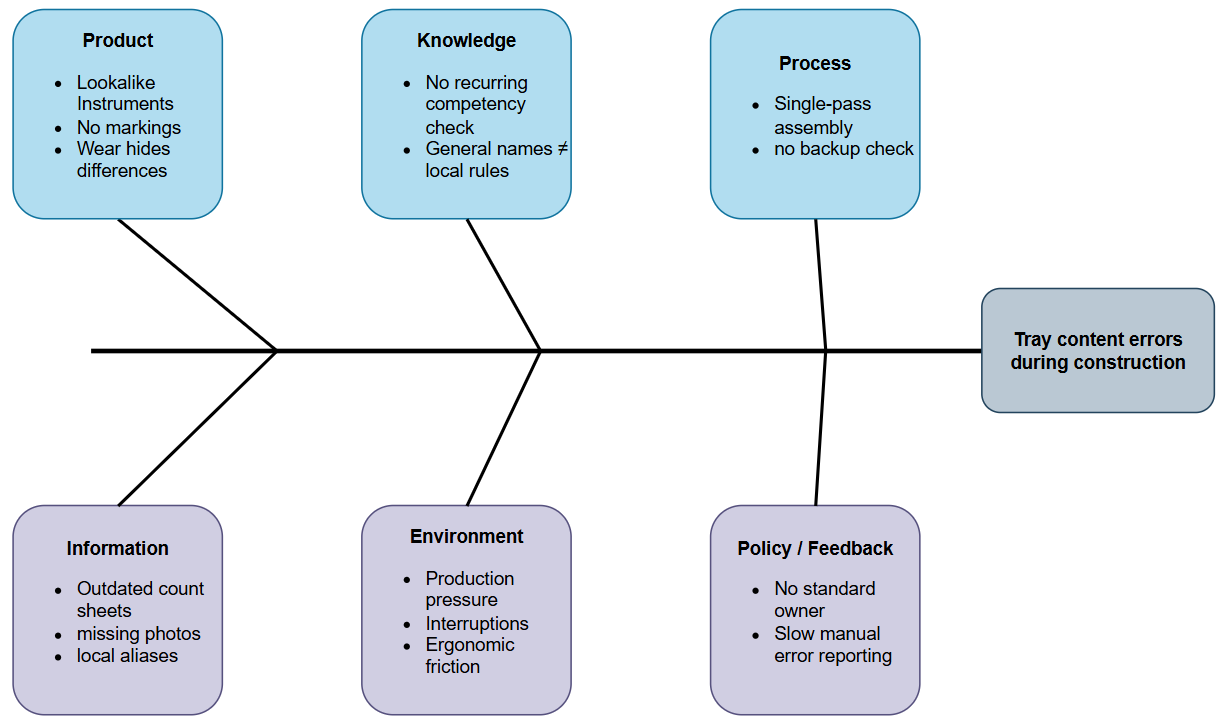
\includegraphics[width=\textwidth]{figures/fishbone_rca.png}
\caption{Fishbone root cause analysis of tray content errors during reconstruction of reusable stainless steel instrument trays.}
\label{fig:fishbone-rca}
\end{figure}

\textbf{Product.}

Same-family instruments (Kelly/Crile, straight/curved Mayo) differ only in
subtle dimensional features with no intrinsic labels or markings
\cite{alfred-et-al-2021, lind-2026a, nichol-et-al-2024, ast-surgical-instrumentation-guide, encyclopedia-surgical-instruments-2018, czarnowski-2025}. For example, a tray requiring four 14~cm Kelly clamps
and two 16~cm Kelly clamps can be misassembled as two 14~cm and four 16~cm
clamps---the total count is correct but the instrument variant is wrong, a pattern
that Zhu et al. found accounted for 44.0\% of all instrument packaging errors
\cite{zhu-et-al-2019}. Steam
autoclaving destroys adhesives and fades inks, laser etching is unstandardized
across manufacturers, and reprocessing wear further reduces visible cues
\cite{infection-control-today-instrument-marking-2017, hspa-instrument-resources-accessed-2026}.

The instrument supply chain evolved around surgical function, not SPD
identification. Manufacturers bear labeling cost, and SPD receives the benefit — but SPD has no purchasing authority over instrument design
\cite{ashcsp-central-service-history}. No stakeholder has enough individual incentive to change instrument-marking practices because error costs are small incremental delays spread across the workflow, not a direct impact on surgery or surgical liability
\cite{association-of-health-care-journalists-2024}. No regulatory body mandates
marking because no sentinel event with a clear causal line to patient death has
been attributed to unlabeled instruments
\cite{joint-commission-sentinel-event-2024}. Retrofitting across existing
inventory is prohibitive.

Tray composition, instrument design, inventory, and unstandardized nomenclature
make each tray a complex product to reconstruct reliably
\cite{alfred-et-al-2021}. Tray contents are local design decisions rather than
fixed universal lists. Procedure-specific, surgeon-specific, and
hospital-specific decisions determine which instruments and quantities belong in
a set \cite{dos-santos-et-al-2021, ahmadi-et-al-2023}. A user can know
instrument families and still select the wrong item or quantity for a given
tray. Reconstruction must also include rejection of visibly unacceptable items,
not only selection of named items. Otherwise damaged or suspect instruments can
remain in a tray despite correct identity and count
\cite{cdc, cdc-healthcare-equipment-accessed-2026, cdc-environmental-surfaces-accessed-2026, steris-cleaning-instruments-accessed-2026, public-health-ontario-2013, pennsylvania-patient-safety-authority-2006, medline-custom-trays-2025, medline-transport-2026}.

\textbf{Knowledge.}

Three sub-causes converge. First, knowing the general name is not sufficient.
Technicians must see the difference between nearly identical instruments
\cite{castillo-gutierrez-2025, nichol-et-al-2024}. Visual discrimination is
a perceptual skill that requires deliberate practice with feedback
\cite{fast-et-al-2019, shreckengost-et-al-2022}, but the SPD workplace
provides no structured opportunity for this practice. Preceptors train on the
fly, production pressure prevents deliberate study, and no mechanism identifies
which visual discriminations an individual has not yet mastered
\cite{nichol-et-al-2024, alfred-et-al-2021}. Certification failure rates of
28--50\% confirm that the technical demands are substantive, yet the role
remains classified and compensated as entry-level support labor
\cite{hspa-crcst-accessed-2026, hspa-crcst-content-outline-2023, hspa-urology-instruments-accessed-2026}.

Second, general instrument knowledge and local tray rules are separate domains.
Manufacturers produce physically different tools under the same generic name
\cite{nadeau-2024}. Tray composition is driven by surgeon preference, hospital
case mix, and historical accretion rather than a universal standard
\cite{dos-santos-et-al-2021, ahmadi-et-al-2023}. Local aliases accumulate
organically on count sheets with no central nomenclature authority
\cite{alfred-et-al-2021}. Count sheets encode tray-specific rules that exist
only in that hospital's workflow \cite{nadeau-2024, purdue-count-sheets-accessed-2026}.

Local tray configurations operate at substantial scale. At Aarhus University Hospital, Denmark's largest hospital, a tray-optimization project catalogued 1,340 instrument trays across 12 surgical specialties and 74 operating rooms, averaging 30 instruments per tray \cite{rubak-et-al-2024}. No single tray design generalized across specialties or procedures; the hospital maintained 258 distinct tray types before optimization. A technician rotating between specialties encounters different tray rules, different instrument sets, and different quantities for each room.

Even within a single tray type, usage varies by case and procedure. At Maastricht University Medical Center in the Netherlands, one Major General Surgery tray contained 94 reusable instruments used across 162 multi-disciplinary procedures \cite{eussen-et-al-2026}. On average only 19 instruments were used per case; 10 were never used across all 162 procedures, and the remaining 65 appeared in fewer than 20\% of cases. Observation-based optimization removed those rarely used instruments, reducing the tray's size and weight by 54\% \cite{eussen-et-al-2026}. A technician cannot rely on frequency of use to know a tray's content.

Third, certification proves a starting point rather than local readiness.
Neither HSPA nor CBSPD mandates recurring competency checks tied to local tray
knowledge
\cite{hspa-crcst-accessed-2026, ofstead-et-al-2023, aorn-staffing-shortage-2025, kovach-2012, nadeau-2017}. Training inconsistency
persists because no single role owns the standard curriculum for each tray.
Differences across clinical supervisors, shifts, and training tenures produce conflicting
mental models of the same tray
\cite{alfred-et-al-2021, hu-et-al-2024, thurmond-2020, lind-2026b}.

\textbf{Process.}

Building a tray forces picking, counting, checking, and arranging into one step
with no double-check system. Alfred et al. found that 55.0 percent of tray
defects occur during assembly
\cite{alfred-et-al-2021}. Nichol et al. found that
88.6 percent of observed errors involve visualization tasks such as inspection,
identification, function checking, and sorting
\cite{nichol-et-al-2024}. Sequential
verification would double labor per tray, and no accreditation mandate from the
Joint Commission, CMS, or HSPA requires a two-person check for tray assembly
\cite{alfred-et-al-2021, chen-et-al-2023, pelzer-et-al-2024}.

Productivity metrics structurally incentivize single-pass assembly. The AAMI
benchmarking framework uses worked-hours-per-unit (WHPU), reinforcing throughput
as the primary performance signal
\cite{kusler-jensen-spd-benchmarking-2023}.
Instrument damage such as corrosion, stains, burrs, and worn jaw serrations can
be missed when inspection relies on rapid visual checks under poor lighting
\cite{lind-2026a}. Workers use only their eyes and hands, without magnification,
side-by-side comparison guides, or decision-support tools at the workstation
\cite{nichol-et-al-2024}. No worker can remember every item in every tray when a
single hospital may manage hundreds of tray configurations, each with 30 to more
than 100 instruments. Production pressure and cognitive load cause workers to
break from the count sheet and rely on memory, especially for familiar trays
\cite{nadeau-2024}. No formal measurement of count-sheet compliance exists, so
the gap between assumed behavior and actual behavior is invisible to management.
Tray errors have not crossed the sentinel-event threshold needed to trigger
regulation \cite{joint-commission-sentinel-event-2024}.

\textbf{Information.}

Count sheets become incomplete or outdated because tray contents change
continuously. Instruments are added, removed, substituted, or replaced as
surgeon preferences shift, manufacturers discontinue items, or vendors supply
new loaners. No dedicated role or budget exists for count-sheet maintenance.
Updating a count sheet is a manual, discretionary task that competes with
production work. Without a formal change-management workflow, sheets accumulate
inaccuracies across multiple revision cycles
\cite{nadeau-2024}. Missing or
outdated identification information, IFUs, and tray listings at the workstation
force workers to rely on memory \cite{lind-2025}.

Loaner trays introduce a separate information failure. They arrive with
manufacturer-stocked contents and vendor documentation that uses the vendor's
naming conventions and part numbers, not the hospital's local aliases or
count-sheet format. SPD receives the tray with hours or minutes to process it
before surgery, and the worker must reconcile the vendor's nomenclature against
the local count sheet with no lead time to prepare or cross-reference
\cite{steris-loaner-trays-2021}.

Automated counting and tracking technologies such as RFID have been explored to reduce tray-reconstruction errors, but adoption remains limited by infrastructure cost for most hospitals \cite{coustasse-et-al-2013, hill-et-al-2022, kusuda-et-al-2024, olivere-et-al-2021}. Sensor-based autonomous verification has also been investigated but requires real-instrument access and deployment validation beyond the current project scope \cite{da-silva-et-al-2026, sayani-et-al-2018}.

\textbf{Environment.}

Multiple environmental conditions reduce the attention and time available for
tray reconstruction. Pressure and interruptions break focus for detail-heavy
visual work
\cite{alfred-et-al-2021, huang-et-al-2025}. The open-plan
workstation layout makes it difficult to shield assembly workers from
interruptions. Phones ring with OR requests, surgeons call for add-on
instruments, and runners deliver and collect trays
\cite{huang-et-al-2025}. Uncomfortable workstations, awkward reaches, and poor
setup make a job that already needs close attention harder
\cite{osha-central-sterile-supply-accessed-2026, cdc-niosh-2024, osha-computer-workstations-accessed-2026}. Ergonomic improvements compete
for facilities budget with clinical areas that have more organizational
visibility. SPD staff have less organizational voice than clinical departments
\cite{surgical-directions-spd-invisible-2025}.

The wage level is a structural cause that amplifies every other category. SPD is
a cost center within the hospital. It generates no direct revenue, so staffing
budgets are structurally constrained relative to OR capacity, which is a revenue
center
\cite{steris-capital-budgeting-2024, moab-healthcare-spd-cost-center-2024}. Hospitals routinely add surgery
suites without proportionally increasing SPD headcount
\cite{ingold-2025}. Average
SPD pay is \$69,217, with a 14 percent drop in respondents receiving raises. SPD
workers describe wages as ``less than your local Starbucks wage''
\cite{nadeau-2023-spd-salary-survey, perry-circulating-life-spd-2022}. Fewer
staff means less time for training and less thorough checking
\cite{alfred-et-al-2021, aorn-staffing-shortage-2025, macola-et-al-2025, brozak-2025, onet-medical-equipment-preparers-accessed-2026}.

Three structural mechanisms---historical classification as materials management,
absence of professional licensure, and low union representation---produce this
wage level. Together they create a self-reinforcing cycle: structural
underinvestment produces low wages, low wages produce chronic vacancies,
vacancies increase production pressure, and production pressure preempts the
training and process improvements that could reduce errors
\cite{evolved-sterile-processing-2025, specialtycare-travel-spd-2026, bls-union-2023, trends-in-labor-unionization-2022, ashhra-2024}.

\textbf{Policy \& Feedback.}

SPD governance is decentralized across shifts. No single role is responsible for
maintaining, auditing, or enforcing count-sheet accuracy or tray-assembly
procedure across all shifts
\cite{nadeau-2024, loria-2024}. Creating a single
authoritative standard for each tray requires a designated owner, a maintenance
process, and enforcement across shifts, but none of these are budgeted.

Certification bodies (HSPA, CBSPD) recommend but do not mandate recurring
competency checks tied to local tray knowledge. When competency programs exist,
they are locally administered with no external audit
\cite{kovach-2012, ofstead-et-al-2023}.
The absence of a mandate means that even published, evidence-backed
training programs --- such as the Ofstead et al.\ (2023) borescope
inspection pilot --- remain discretionary investments that compete
for budget with production headcount, rather than required practice.

Error reporting is manual, slow, and deprioritized. Errors discovered during
surgery are documented, if at all, in incident reports that may take weeks to
reach SPD management. By that time the specific tray, technician shift, and
training gap are hard to identify, so the error teaches no preventive lesson
\cite{nichol-et-al-2024, zhu-et-al-2019}. The hospital incident reporting
system was designed for clinical errors such as medication errors, falls, and
wrong-site surgery. Tray-content errors do not fit neatly into the reporting
categories, so they are underreported. Without closed-loop tracking that ties an
error back to a root cause, downstream detection does not drive upstream
improvement \cite{nichol-et-al-2024, zhu-et-al-2019}.

Structured process-improvement approaches can substantially reduce these
defects. Using Six Sigma methodology, Natarus et al. improved first-pass yield
from 81.0\% to 97.4\% and reduced the tray defect rate from 2.2\% to less than
0.1\% in a hospital sterile-processing department, demonstrating that targeted
workflow and training interventions can close the gap described above
\cite{natarus-et-al-2025}.

\textbf{Consolidated Root Cause Chain.}

Sterile processing evolved from materials management, producing a logistics-oriented workforce without the professional infrastructure of clinical departments.
Compensation and professional infrastructure reflect that origin: below current technical demands.
Hospital associations resisted mandatory certification because it would create upward wage pressure.
Low union representation leaves no institutional mechanism to counter cost-center budget logic.
Temporary contract SPD technicians earn 40 to 80 percent more than permanent staff \cite{nadeau-2023-spd-salary-survey, specialtycare-travel-spd-2026}.

Compounding these workforce conditions, the hospital financial structure separates OR revenue from SPD cost: every SPD investment is visible as expense while error reduction has no standard metric.
Hospitals add surgery suites without increasing SPD headcount, making underinvestment rational at each hospital because error costs are diffuse workflow friction.

A third structural driver compounds the first two: no information architecture connects OR outcomes to SPD actions, so upstream errors have no downstream feedback.

A cross-profession comparison confirms that these structural drivers,
not the quality of available evidence, explain the absence of reform.
Respiratory therapy followed the canonical professionalization
trajectory: the American Association for Respiratory Care (AARC)
established a voluntary certification in 1969, unified credentialing
under the National Board for Respiratory Care in 1974, and then
lobbied state legislatures one by one; California passed the first
licensure law in 1982, and by 2004 all 48 contiguous states had
enacted licensure for respiratory therapists, enforced by state boards
with disciplinary authority
\cite{aarc-timeline}.
Surgical technology is mid-trajectory: the Association of Surgical
Technologists (AST) has driven over a dozen states to require
graduation from a CAAHEP-accredited program and Certified Surgical
Technologist (CST) credentialing, though many states still lack
regulation
\cite{ast-state-laws}.

Sterile processing followed none of this path, and the reason is not
that its technical demands are lower. A comparison of enabling
conditions makes the gap explicit:

\begin{table}[H]
\centering
\caption{Enabling conditions for professionalization: respiratory therapy, surgical technology, and sterile processing}
\label{tab:professionalization-enabling-conditions}
\small\renewcommand{\arraystretch}{1.2}\setlength{\tabcolsep}{4pt}
\begin{tabularx}{\textwidth}{|>{\raggedright\arraybackslash}p{2.5cm}|>{\raggedright\arraybackslash}X|>{\raggedright\arraybackslash}X|>{\raggedright\arraybackslash}X|}
\hline
Enabling condition & Respiratory therapy & Surgical technology & Sterile processing \\
\hline
Visible patient harm creating political will & Respiratory-failure patient deaths drove legislative urgency & Surgical-site infection outbreaks provided the harm narrative & Tray-content errors have not crossed the sentinel-event threshold \cite{joint-commission-sentinel-event-2024} \\
\hline
Professional association with lobbying infrastructure & AARC maintains full-time government-affairs staff and drafts model legislation \cite{aarc-timeline} & AST runs a sustained state-by-state legislative campaign \cite{ast-state-laws} & HSPA and CBSPD are voluntary certification bodies, not advocacy organizations \\
\hline
Standardized education pipeline & CoARC-accredited programs are the required entry path & CAAHEP-accredited programs required by law in regulated states & No mandated program accreditation; 400 hands-on hours with no curriculum standard \\
\hline
Direct patient-care lineage & Evolved from ICU respiratory support (1950s--60s) & Evolved from intraoperative assistance in the OR & Evolved from central supply and materials management \cite{ashcsp-central-service-history} \\
\hline
\end{tabularx}
\end{table}

Each condition maps to a structural driver identified above. The
absence of visible harm corresponds to the broken feedback loop that
keeps error costs invisible. The absence of lobbying infrastructure
and education standardization corresponds to the weak
professionalization that followed from SPD's materials-management
origin. The absence of a patient-care lineage corresponds to the
cost-center classification that suppresses wages and organizational
voice. Together these explain why a role with comparable technical
demands remains a semi-profession while adjacent roles achieved
state-enforced regulation \cite{etzioni-semi-professions-1969}.

No information architecture connects downstream OR outcomes to upstream SPD
actions. The feedback loop from error to correction is broken, so the same
failures repeat without triggering systemic change. Error reporting is designed
for clinical events, not tray-content errors.

The system remains stable because no stakeholder has both the incentive and the
authority to change it. Manufacturers control instrument design but bear no cost
from SPD identification errors. Hospital administrators control SPD budgets but
see wage increases as expense and error costs as invisible friction. SPD
workers perform the work but lack the union representation, professional
licensure, or organizational voice to demand structural change. Regulatory
bodies have not acted because tray errors have not crossed the sentinel-event
threshold.

% ── Section 3 ──

\section{First Attempt: A Computer-Vision Tray Checker \hfill {\normalfont\small (Matthew, Qiyu)}}
\label{sec:first-attempt-a-computer-vision-tray-checker}
\subsection{CV Literature Context}

Computer vision was selected as the initial approach because published work
showed that automated surgical-instrument detection and counting could work in
experimental settings. Deol et al. trained a deep-learning detector on 1,004
images of 11 instrument categories and reported 98.5\% precision and 99.9\%
recall on static images with real-time inference at 40~FPS
\cite{deol-et-al-2024}. Atabuzzaman et al.
built a multi-view CNN-transformer system for 95 instrument subtypes across
three surgical trays and demonstrated improved CSSD workflow efficiency in a
deployed user study
\cite{atabuzzaman-et-al-2025}. These papers supported CV as a candidate for tray
verification. The YOLO architecture used in these studies originated as a
unified real-time detection framework \cite{redmon-et-al-2016}, and
surgical-instrument datasets continue to expand the class coverage
available for training \cite{rodrigues-et-al-2022a}.
\subsection{Requirements and System Design}
\label{sec:requirements-and-system-design}

Four operational requirements constrained the original CV-based tray-checker
design. First, the system had to run entirely on local hardware in the SPD.
Hospital IT environments rarely provide GPU-equipped
workstations~\cite{grossi-et-al-2021, chomutare-et-al-2022}, and capital
budgets favor sterilization equipment over departmental computing
hardware~\cite{natarus-et-al-2025}. Second, patient privacy required that
tray images never leave the SPD: images could identify specific procedures,
surgeons, and OR schedules, and HIPAA-covered entities must evaluate even
indirect identifiers before transmitting data
off-site~\cite{khalid-et-al-2023}. Third, the detection pipeline needed to
handle the variable illumination, reflective tray surfaces, and overlapping
tool layouts that SPD workflows present. Fourth, the system had to
incorporate human judgment for uncertain cases and require explicit final
sign-off, supporting rather than replacing the technician.

The local-inference and privacy requirements drove the capture-fixture design.
A fixed overhead camera mounted on a portable weighted board preserved
repeatable camera geometry across work surfaces without cloud connectivity or
GPU infrastructure.

The detection design addressed the robustness requirement through a YOLO object
detector with a two-threshold confidence band, drawing on the
selective-classification literature in which a model abstains rather than
forcing a low-confidence prediction \cite{geifman-and-el-yaniv-2017}.
Detections above a high threshold \(T_{\text{present}} = 0.8\) were accepted as
present; detections between the low threshold \(T_{\text{review}} = 0.3\) and
\(T_{\text{present}}\) triggered a human review state; and the absence of any
candidate above \(T_{\text{review}}\) prompted a rescan or missing-item
recommendation. The review band was designed to be wide in order to accommodate the
miscalibration that object detectors exhibit near their decision boundary
\cite{kuppers-et-al-2022, guo-et-al-2017}, and the operating point would be refined after
training on instrument-specific data. The initial thresholds were chosen to
prioritize precision for the ``present'' decision, following the principle
that safety-critical applications require a higher confidence bar than
benchmark-default values \cite{wenkel-et-al-2021}.

These thresholds defined a four-state tray-status machine
(Table~\ref{tab:original-planned-tray-status-logic}).

The human-in-the-loop and robustness requirements shaped the technician-facing
UI (Table~\ref{tab:original-planned-technician-ui-requirements}).

\begin{table}[H]
\centering
\caption{Original planned tray-status logic using two-threshold confidence band}
\label{tab:original-planned-tray-status-logic}
\small\renewcommand{\arraystretch}{1.2}\setlength{\tabcolsep}{4pt}
\begin{tabularx}{\textwidth}{|>{\raggedright\arraybackslash}X|>{\raggedright\arraybackslash}X|}
\hline
User-Facing State & Decision Logic \\
\hline
\texttt{Present} & Required class has at least required count of detections above high threshold \texttt{T\_present}, no active similar-class or image-quality risk flag, and duplicate boxes reconciled. \\
\hline
\texttt{Needs Review} & Detections between \texttt{T\_review} and \texttt{T\_present}, similar class appears, count unstable, unknown or extra object plausible, or scan quality degraded. \\
\hline
\texttt{Missing} & No candidate above low threshold \texttt{T\_review}, and scan quality acceptable enough that absence is meaningful. \\
\hline
\texttt{Rescan Recommended} & System lacks evidence but glare, occlusion, blur, poor framing, or lighting makes a missing label unsafe. \\
\hline
\end{tabularx}
\end{table}

\begin{table}[H]
\centering
\caption{Original planned technician UI requirements}
\label{tab:original-planned-technician-ui-requirements}
\small\renewcommand{\arraystretch}{1.2}\setlength{\tabcolsep}{4pt}
\begin{tabularx}{\textwidth}{|>{\raggedright\arraybackslash}X|>{\raggedright\arraybackslash}X|>{\raggedright\arraybackslash}X|}
\hline
Requirement & Design Direction & Rationale \\
\hline
One primary action per state & Show the next meaningful action: start scan, rescan, review issue, confirm tray, or stop. & The technician's decision depends on the tray state; surfacing all controls buries the relevant one \cite{amershi-et-al-2019}. \\
\hline
Clear tray-status hierarchy & Summarize Complete, Missing, Extra, and Needs Review above detailed detections. & The tray outcome is the priority; detection details support investigation. \\
\hline
Fast correction and rescan & Provide direct correction, dismiss, and rescan paths instead of forcing a workflow restart. & A workflow restart wastes time and discourages correction. \\
\hline
Specific review reasons & Label review prompts with the cause: low confidence, similar-class risk, glare, overlap, unknown object, or count mismatch. & The technician can accept, dismiss, or rescan without guessing the review trigger. \\
\hline
Visual-first feedback with optional sound & Persistent visible status as the source of truth; short optional audio for major state changes. & Visual status provides a continuously available source of truth independent of SPD noise. \\
\hline
Alert restraint & Escalate only conditions that change the tray decision or require user action. & Conditions that do not change the tray decision do not warrant escalation. \\
\hline
Human sign-off & Require explicit final confirmation. The system supports the decision, not silently makes it. & The system supports the decision, not silently makes it \cite{fda-human-factors-accessed-2026}. \\
\hline
Manual fallback & Make it clear how to continue if camera, model, or scan quality is unavailable. & Tray processing cannot halt when the capture fixture, model, or scan is unavailable. \\
\hline
\end{tabularx}
\end{table}

\subsection{CV Experiments and Results}
\label{sec:computer-vision-experiments}

The published literature established that deep-learning object detectors
can recognize surgical instruments with high accuracy in controlled
settings~\cite{deol-et-al-2024, atabuzzaman-et-al-2025}. Those results
were obtained under fixed lighting, non-reflective surfaces, and separated
instrument layouts---conditions that do not reflect the variability of
real SPD workflows.

Domain shifts in illumination, background appearance, and object
arrangement degrade detection even for models that perform well on matched
benchmarks~\cite{ahmed-et-al-2021, yang-et-al-2024}. Specular reflections
from metallic surfaces further reduce
accuracy~\cite{jayasinghe-et-al-2023, wang-et-al-2016, wei-et-al-2018}, and
object detectors tested under lighting perturbations show significant
performance loss~\cite{premakumara-et-al-2023}. No prior study had
systematically measured how these factors interact for surgical-instrument
detection in an SPD-like setting.

We designed staged experiments testing detection robustness along three
axes directly relevant to SPD conditions: illumination (800--80~lumens),
surface reflectivity (matte vs.\ reflective backgrounds), and layout
occlusion (separated vs.\ overlapping). All experiments used YOLO11s on a
controlled self-collected dataset with five classes (four spoon variants and a fork) arranged in a fixed 11-step brightness ladder across two
background conditions and two layout conditions. Each stage contained 3--43
training images (47--109 total images per stage). The design isolated each
variable independently rather than mixing effects. Published studies report
mAP50 exceeding 0.99 for surgical-instrument detection under controlled
lighting and layout~\cite{deol-et-al-2024, atabuzzaman-et-al-2025}; our
experiments test whether that accuracy holds under SPD-relevant variations.
\paragraph{Architecture selection.}
The staged experiments all used YOLO11s at 640$\times$640~px. This
configuration was selected through a controlled architecture sweep on the
Lavado surgical-instrument dataset. We evaluated four YOLO11 variants (n,
s, m, l) at 640~px and selected variants at 960~px alongside RT-DETR-l, a
Transformer-based real-time detector~\cite{zhao-et-al-2024-rtdetr}, to
assess the accuracy-latency tradeoff at higher input resolution
(Table~\ref{tab:architecture-sweep}). YOLO11s at 640~px was chosen for the
remainder of the experiments: it achieved the best balance of mAP50-95
(0.928) and latency (4.2~ms), and higher-resolution variants offered
marginal accuracy gains at substantially higher compute cost.

\begin{table}[H]
\centering
\caption{Architecture sweep on Lavado dataset}
\label{tab:architecture-sweep}
\small\renewcommand{\arraystretch}{1.2}\setlength{\tabcolsep}{4pt}
\begin{tabularx}{\textwidth}{lrrrrr}
\hline
Model & Precision & Recall & mAP50 & mAP50-95 & Latency (ms) \\
\hline
YOLO11n (640px) & 0.936 & 0.939 & 0.980 & 0.914 & 2.4 \\
YOLO11s (640px) & 0.958 & 0.944 & 0.986 & 0.928 & 4.2 \\
YOLO11s (960px) & 0.965 & 0.968 & 0.990 & 0.948 & 7.1 \\
YOLO11m (640px) & 0.979 & 0.952 & 0.991 & 0.940 & 6.8 \\
YOLO11m (960px) & 0.974 & 0.958 & 0.991 & 0.945 & 14.6 \\
YOLO11l (640px) & 0.964 & 0.949 & 0.988 & 0.932 & 8.0 \\
YOLO11l (960px) & 0.963 & 0.960 & 0.990 & 0.940 & 17.8 \\
RT-DETR-l (640px) & 0.993 & 0.991 & 0.991 & 0.957 & 12.4 \\
\hline
\end{tabularx}
\end{table}

\paragraph{Lavado baseline.}
A YOLO11s model was also trained on the Lavado surgical-instrument
dataset: 2,106 training images across four real instrument classes
(scalpel, straight dissection clamp, straight Mayo scissors, curved
Mayo scissors). After 100 epochs the model achieved precision of 0.972,
recall of 0.978, mAP50 of 0.991, and mAP50-95 of 0.945 on the held-out
test set (302 images). Per-class AP50/AP50-95: Scalpel n4 (0.995/0.929),
Straight Dissection Clamp (0.983/0.892), Straight Mayo Scissor
(0.993/0.977), Curved Mayo Scissor (0.994/0.982). This established that
the training pipeline and architecture perform competitively on a
published surgical-instrument dataset, consistent with prior work on
CNN-based surgical instrument recognition~\cite{lehr-et-al-2023}, before
the staged proxy experiments.
\paragraph{Brightness degradation.}
Two experiments measured monotonic mAP50-95 decay as the train--test
illumination gap widened. \texttt{brightest\_train\_darker\_test} trained
on 800-lumen separated images and tested across all dimmer levels,
producing mAP50-95 of 0.815. \texttt{darkest\_train\_brighter\_test}
trained on 80-lumen separated images and tested across all brighter
levels, producing mAP50-95 of 0.822. The decay was asymmetric: the
brightest-trained model retained higher recall under moderate drops,
while the darkest-trained model recovered more quickly as light
increased. Per-brightness metrics confirmed the trend was consistent
across both matte and reflective backgrounds.
\paragraph{Background transfer.}
Two experiments tested whether the model learned object shape or
overfit to the scene background. \texttt{matte\_train\_reflective\_test}
trained on matte-background images and tested on reflective-background
images across all brightness levels, producing mAP50-95 of 0.776.
\texttt{reflective\_train\_matte\_test} trained on reflective-background
images and tested on matte-background images, producing mAP50-95 of
0.826. The reflective-to-matte direction was stronger, suggesting that
reflective training data provides broader feature invariance.
\paragraph{Occlusion stress.}
The separated-to-overlay layout shift produced the largest degradation.
\texttt{separated\_train\_overlay\_test} trained on non-overlapping
layouts and tested on overlapping layouts, producing mAP50-95 of 0.478
compared with 0.995 on the matched-condition baseline. This gap was
consistent across all brightness ranks and both backgrounds, showing
that training on neatly arranged instruments does not transfer to
cluttered arrangements. The overlay condition was the only experiment
where recall fell below 0.70, making it the clearest product boundary:
the system should request a rescan whenever tools overlap.

Per-image analysis confirms the failure pattern: in the overlay condition
on matte backgrounds, the model detects 2 of 5 instruments on average
(recall~0.4) with zero false positives across all brightness levels. On
reflective backgrounds, recall rises to 0.8 with occasional false
positives. The dominant failure mode is systematic under-detection
rather than spurious extra predictions.

\begin{table}[H]
\centering
\caption{Aggregate test-set metrics for the seven staged brightness experiments}
\label{tab:brightness-stage-metrics}
\small\renewcommand{\arraystretch}{1.2}\setlength{\tabcolsep}{4pt}
\begin{tabularx}{\textwidth}{lrrrr}
\hline
Stage & Precision & Recall & mAP50 & mAP50-95 \\
\hline
\texttt{brightest\_train\_darker\_test} & 0.898 & 0.953 & 0.993 & 0.815 \\
\hline
\texttt{darkest\_train\_brighter\_test} & 0.955 & 1.000 & 0.984 & 0.822 \\
\hline
\texttt{bright\_train\_dim\_test} & 0.992 & 0.992 & 0.995 & 0.904 \\
\hline
\texttt{dim\_train\_bright\_test} & 0.907 & 0.851 & 0.995 & 0.886 \\
\hline
\texttt{matte\_train\_reflective\_test} & 0.915 & 0.904 & 0.957 & 0.776 \\
\hline
\texttt{reflective\_train\_matte\_test} & 0.832 & 0.893 & 0.975 & 0.826 \\
\hline
\texttt{separated\_train\_overlay\_test} (overlay) & 0.836 & 0.671 & 0.716 & 0.478 \\
\hline
\texttt{separated\_train\_overlay\_test} (baseline) & 0.998 & 1.000 & 0.995 & 0.995 \\
\hline
\end{tabularx}
\end{table}

\begin{figure}[H]
\centering
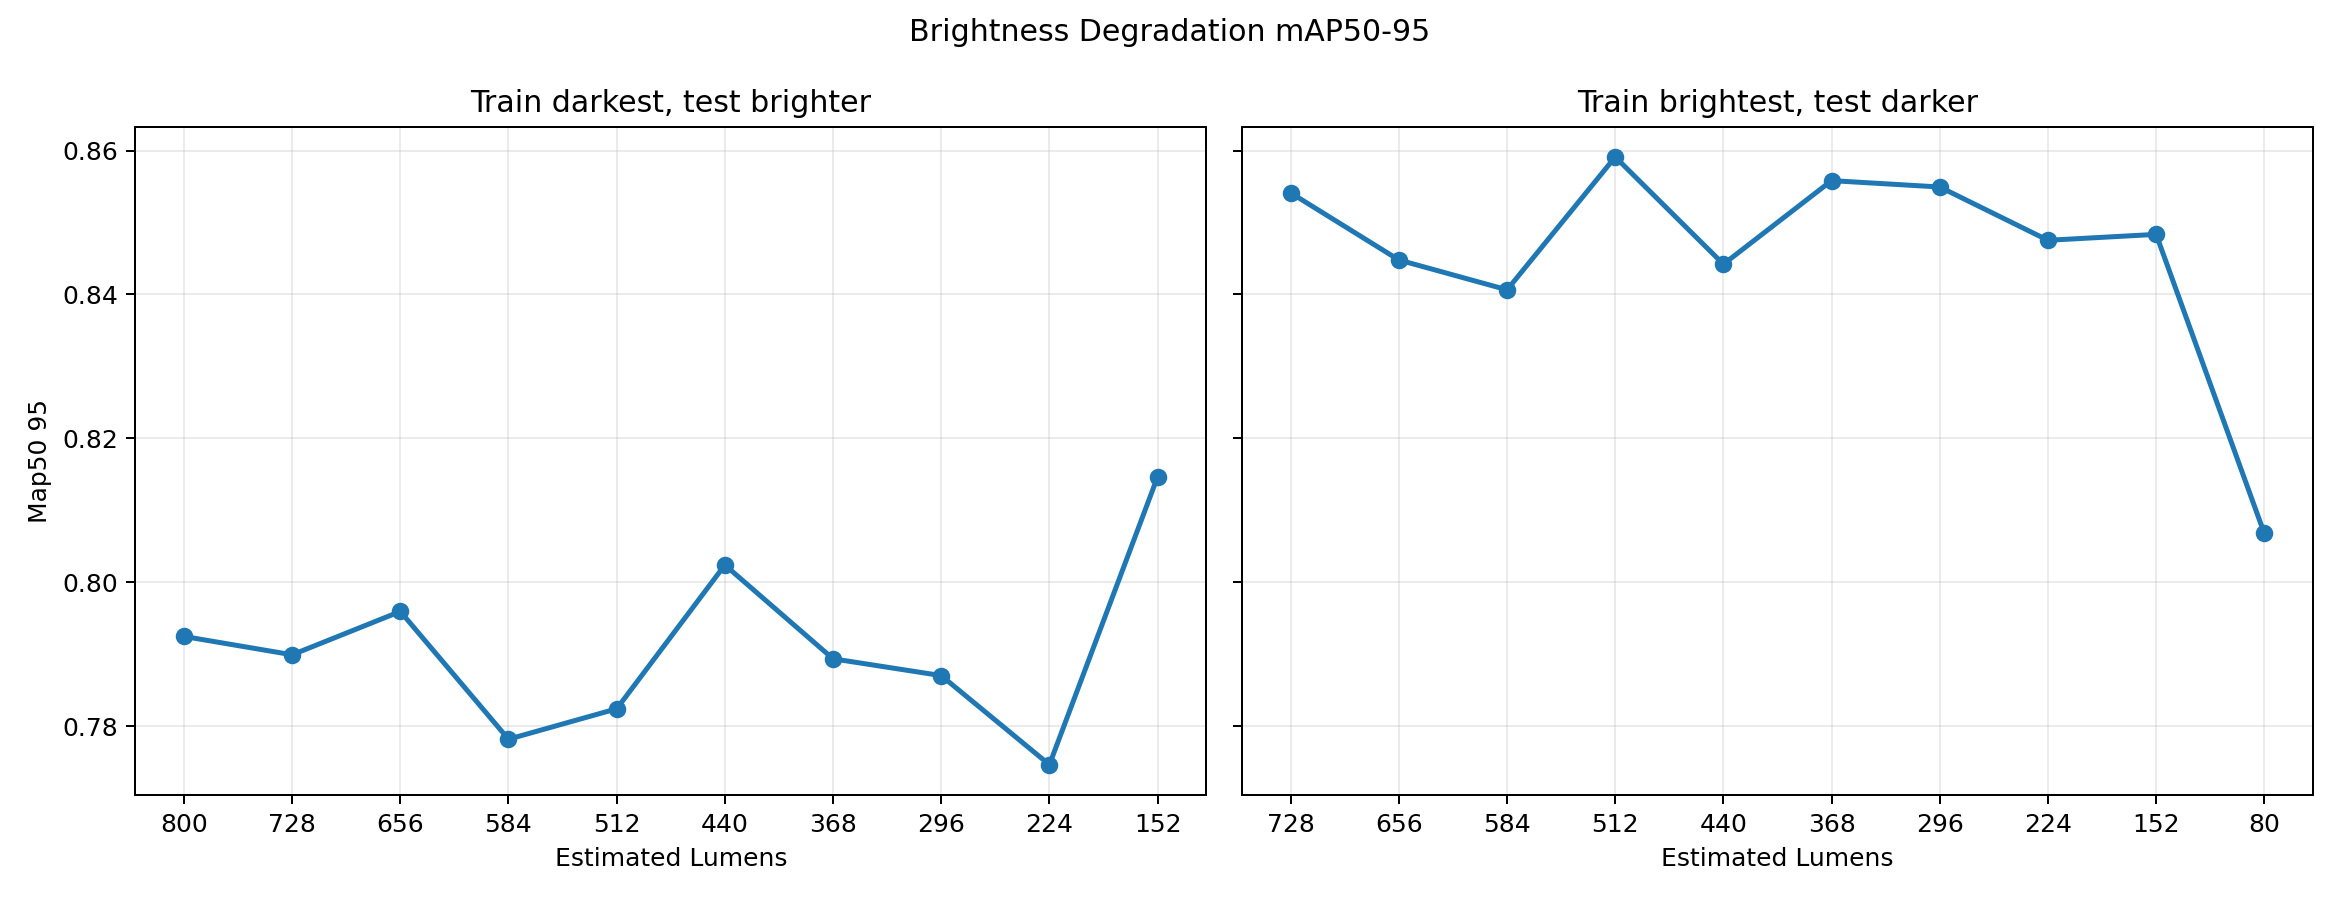
\includegraphics[width=\textwidth]{figures/brightness_map50_95_panels.png}
\caption{Brightness degradation mAP50-95 across the estimated-lumens range. Left panel: model trained on darkest (80~lumens), tested on brighter levels. Right panel: model trained on brightest (800~lumens), tested on dimmer levels.}
\label{fig:brightness-decay}
\end{figure}

\begin{figure}[H]
\centering
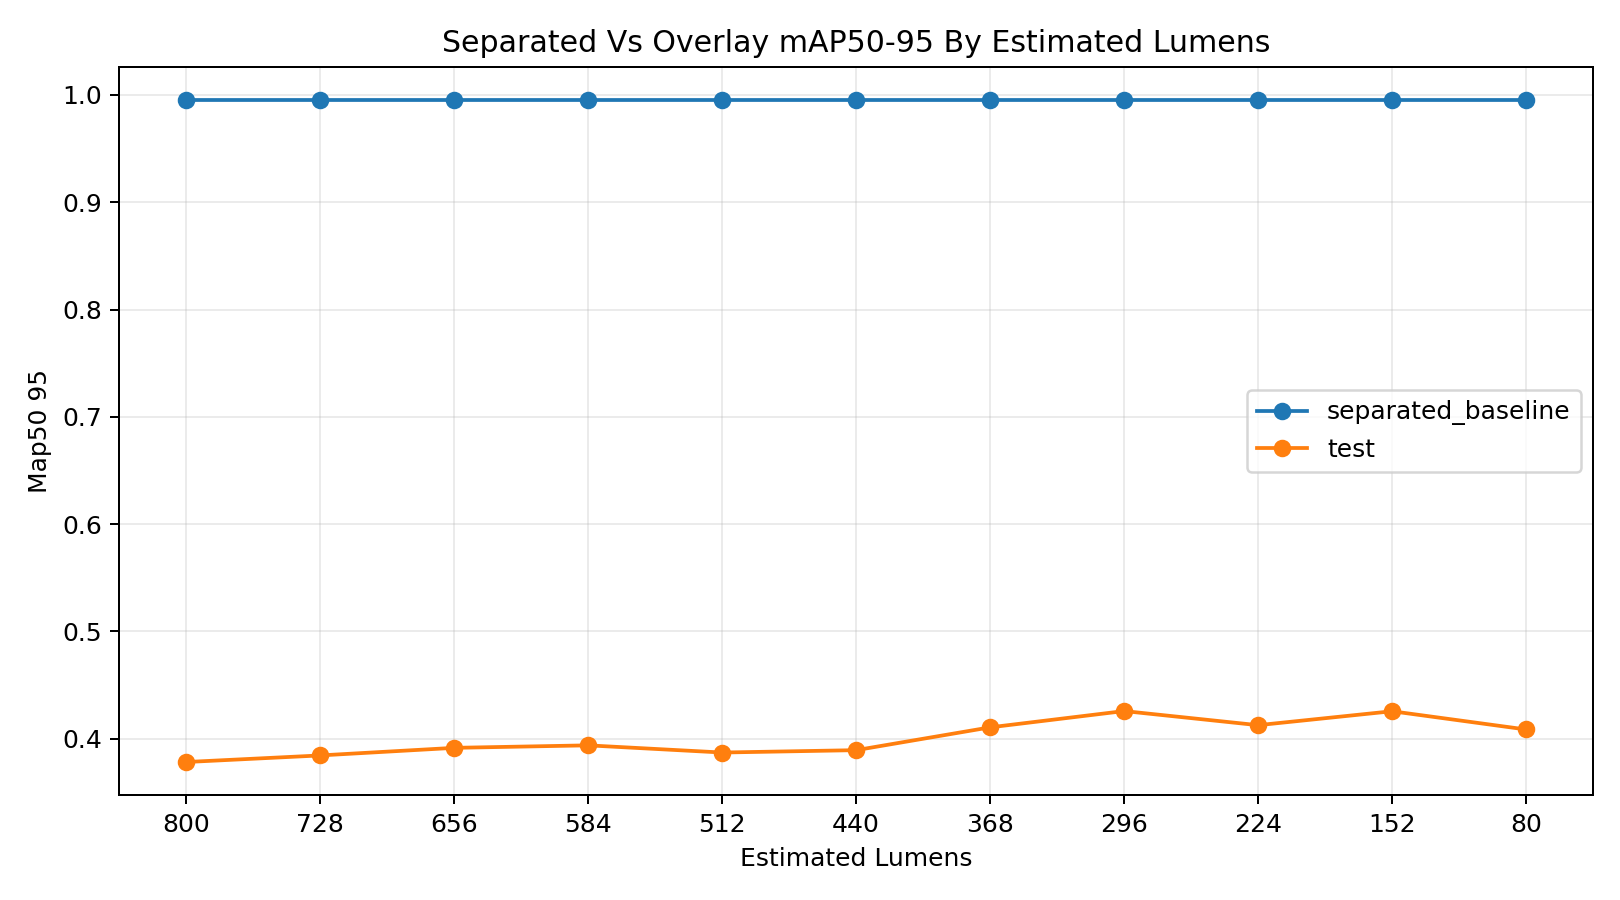
\includegraphics[width=\textwidth]{figures/overlay_map50_95.png}
\caption{Separated versus overlay layout: mAP50-95 across the estimated-lumens range. The overlay condition produces the largest degradation (mAP50-95~=~0.478).}
\label{fig:overlay-degradation}
\end{figure}

\paragraph{Real-instrument experiments.}
The brightness experiments above used a spoon proxy to measure
degradation under controlled variables. A further set of experiments
tested detection on real surgical instruments---six classes
(scissor1--4, forcep, scalpel) from a surgical training kit photographed
on matte and reflective backgrounds across four sessions. Three staged
experiments were trained for 100~epochs each using YOLO11s and
validated on held-out sessions:

\begin{table}[H]
\centering
\caption{Aggregate test-set metrics for the three real-instrument experiments}
\label{tab:surgical-kit-stage-metrics}
\small\renewcommand{\arraystretch}{1.2}\setlength{\tabcolsep}{4pt}
\begin{tabularx}{\textwidth}{lrrrr}
\hline
Stage & mAP50 & mAP50-95 & P & R \\
\hline
\texttt{matte\_train\_reflective\_test} & 0.336 & 0.233 & 0.425 & 0.236 \\
\texttt{reflective\_train\_matte\_test} & 0.160 & 0.119 & 0.123 & 0.160 \\
\texttt{shape\_similarity\_real\_proxy} & 0.300 & 0.253 & 0.239 & 0.347 \\
\hline
\end{tabularx}
\end{table}

These scores are substantially lower than the spoon-proxy results.
Per-class analysis (Table~\ref{tab:app-surgical-kit-per-class}) reveals
a systematic pattern: each image contains exactly six instruments in fixed
positions per session, so a model can learn which classes appear at which
image locations rather than learning visual features. Different classes
survive under different splits---scissor1 reaches 0.862~AP under the
shape-similarity split but falls to 0.000 under lighting transfer splits,
while forcep and scissor2 follow the opposite pattern. Only scalpel, the
most visually distinct instrument (single blade vs.\ multi-loop scissors),
transfers across conditions (0.717~AP in reflective-to-matte). The
confusion matrix (Figure~\ref{fig:app-confusion}) confirms that missed
detections are the dominant failure mode: when the model fails, it
produces a false negative rather than a false positive. The lighting
transfer experiments are therefore confounded by position-cue leakage:
the test metric reflects both lighting difficulty and layout
generalization. These results motivated the pivot to a training
platform where controlled physical cards replace uncontrolled
instrument recognition.

A separate experiment confirmed that adding lighting variety during
training improves held-out-condition detection
(Appendix~\ref{sec:appendix-c-lighting-diversity}).

\paragraph{Lessons learned.}
\label{sec:boundary-conditions-for-future-cv-work}
Detection worked reliably in controlled, matched-condition settings and degraded under
every variation that SPD workflows present---variable illumination
(mAP50-95 as low as~0.822), reflective tray surfaces (mAP50-95 as low
as~0.776), and overlapping instruments (mAP50-95~=~0.478). The real-instrument
experiments were confounded by position-cue leakage and failed to transfer
across lighting conditions. These results showed that a CV-only tray checker
could not deliver reliable detection under SPD conditions within the project's
timeline and resources.
Controlled lighting and layout are prerequisites for
reliable detection. The training-centered pivot is the subject of
Section~\ref{sec:reason-for-pivot}.

\subsection{CV Requirements Assessment and Gap Analysis}
\label{sec:cv-gap-analysis}

The original tray-verification concept defined requirements for automated
tray-status logic, technician-facing UI, physical capture fixture, and
detection reliability. Each requirement is assessed below.

\begin{table}[H]
\centering
\caption{CV design outcome versus requirements}
\label{tab:cv-design-outcome-versus-requirements}
\small\renewcommand{\arraystretch}{1.2}\setlength{\tabcolsep}{4pt}
\begin{tabularx}{\textwidth}{|>{\raggedright\arraybackslash}X|>{\raggedright\arraybackslash}X|>{\raggedright\arraybackslash}X|>{\raggedright\arraybackslash}X|}
\hline
Requirement & Target & Achievement & Gap \\
\hline
Tray-status logic with two-threshold confidence band & Present, Needs Review, Missing, Rescan states & Logic specified and documented & Not tested with real SPD workflow data \\
\hline
Technician-facing UI with one primary action per state & Clear hierarchy, fast correction, specific review reasons, human sign-off & UI requirements specified & Not implemented beyond design documentation \\
\hline
Physical capture fixture & Overhead camera on portable weighted board & Fixture design documented & Not fabricated or tested in SPD conditions \\
\hline
Lighting robustness & Detection maintains mAP50 above 0.7 across SPD-like illumination range & Evaluated across 800--80 lumens; overlay layout caused largest drop & mAP50-95=0.478 in overlay condition; lighting still a deployment barrier \\
\hline
Lookalike discrimination & Correctly distinguish straight/curved, narrow/broad same-family pairs & Evaluated with 6 real instrument classes (scissor1--4, forcep, scalpel) & Per-class AP varies by split from 0.000 to 0.862; position cues dominate over shape; only visually distinct scalpel transfers reliably \\
\hline
Open-set rejection & Detect unknown objects as unfamiliar rather than assigning spurious labels & \multicolumn{2}{>{\raggedright\arraybackslash}X|}{Not evaluated --- no distractor dataset available; open-set recognition methods exist but require threshold calibration~\cite{scheirer-et-al-2013, schlachter-et-al-2020}} \\
\hline
Synthetic-to-real transfer & Synthetic pretraining enables few-shot real deployment & \multicolumn{2}{>{\raggedright\arraybackslash}X|}{Not evaluated --- no 3D instrument models available for synthetic data generation; few-shot detection approaches~\cite{wang-et-al-2020-fsod} could reduce annotation burden} \\
\hline
\end{tabularx}
\end{table}

The training-centered pivot (Section~\ref{sec:reason-for-pivot}) preserved the project's technical contributions
(the CV experiments, data collection pipeline, and detection code are
documented in Section~\ref{sec:first-attempt-a-computer-vision-tray-checker})
while replacing the main evidence path with a claim that was buildable,
testable, and interpretable within the project's resources. The CV infrastructure
remains available as a future support layer after separate validation
(Section~\ref{sec:boundary-conditions-for-future-cv-work}).

\subsection{CV Implementation Summary}

The following CV subsystems were implemented:

\begin{itemize}
   \item \textbf{Data collection and annotation pipeline.} A webcam capture tool with bounding-box annotation UI supports rapid multi-session data collection with per-class image output, YOLO label export, and session save/load (\texttt{src/trayguard/data\_collection/}).
   \item \textbf{Training infrastructure and benchmark harness.} A Hydra-configured training pipeline supports model, dataset, and hyperparameter overrides across YOLO11n/s/m/l variants and RT-DETR-l, with a multi-variant benchmark for accuracy--latency comparison (\texttt{src/trayguard/training/}).
   \item \textbf{Legacy tray-check demo.} A live YOLO tray-check interface demonstrates camera capture, detection, and tray-status comparison for proof-of-concept review (\texttt{src/trayguard/app/streamlit\_app.py}).
\end{itemize}

\subsection{Limitations of the CV Experiments}

The CV experiments have several constraints that limit the strength of
their conclusions. First, the brightness and occlusion experiments used a
spoon proxy rather than real surgical instruments. While the proxy
controlled for confounds such as shape and reflectivity variation, it does
not capture the fine-grained visual differences between functionally
similar instrument classes that fine-grained classification methods
address~\cite{wang-et-al-2021, zhao-et-al-2017, seeland-and-mader-2021},
and the degradation magnitudes may differ from
those of real instruments under identical conditions. Second, the real-
instrument experiments were confounded by position-cue leakage: the
testing layout used fixed positions per session, so the model learned
spatial correlations rather than visual features alone, making the
lighting-transfer results difficult to interpret (Section~\ref{sec:computer-vision-experiments}).
Third, all experiments used a single architecture (YOLO11s) and a single
training recipe. The architecture sweep
(Table~\ref{tab:architecture-sweep}) identified YOLO11s as the best
accuracy--latency balance from eight configurations, but the broader
conclusions rely on a single detection architecture; other detectors,
pretraining strategies, or data-augmentation pipelines may produce
different degradation patterns, and ML
reproducibility concerns~\cite{heil-et-al-2021, tikhomirov-et-al-2026}
apply to any single-site evaluation. Fourth,
the test conditions---staged brightness ladders, fixed layouts, and
controlled backgrounds---do not reproduce the full variability of real SPD
workflows, including arbitrary instrument arrangements, occlusion challenges
documented in the detection literature~\cite{ning-et-al-2021}, open-set
distractors, dirt or wear, and operator-induced framing variation. Fifth,
the Lavado baseline and real-instrument experiments covered at most six
classes, whereas a deployment-ready system would need to distinguish
hundreds of instrument types across multiple manufacturers. The evidence supports bounded claims about
degradation patterns in proxy settings.

% ── Section 4 ──

\section{Literature And Related Work \hfill {\normalfont\small (Matthew, Andy, Qiyu)}}
\label{sec:literature-and-related-work}
\label{sec:reason-for-pivot}

The CV-first attempt did not produce a deployable verification system within the project's constraints. Returning to the root causes identified in the RCA (Section~\ref{sec:root-cause-analysis}), the team revisited the solution space and identified seven intervention points. The following literature examines each relevant area and supports the selected path.

\subsection{The Solution Landscape}
\label{sec:solution-landscape}

The solution space for reducing tray-content errors during reconstruction can
be organized into seven categories by intervention point. Each category targets
a different subset of the root causes, and each faces a
different feasibility constraint for this project.

The seven identified solution categories are:
\begin{enumerate}
  \item \textbf{Automated content verification}: post-assembly inspection using CV, RFID, or barcode scanning to verify tray contents.
  \item \textbf{Physical error-proofing}: modifying the tray or instrument interface (custom foam, color coding) to prevent selection errors.
  \item \textbf{Workflow / process design}: restructuring task handoffs and verification steps through dual checks or gating sign-offs.
  \item \textbf{Decision support at point of assembly}: providing standardized count sheets, photos, and alias lookup at the workstation.
  \item \textbf{Task simplification}: rationalizing tray contents and standardizing instrument sets across procedures.
  \item \textbf{Workforce / accountability systems}: competency reassessment, closed-loop error tracking, and structured mentorship.
  \item \textbf{Training and simulated practice}: building local tray skills through retrieval practice, simulation, and feedback before supervised work.
\end{enumerate}

\begin{table}[H]
\centering
\caption{Seven solution categories compared by constraint}
\label{tab:seven-solution-categories-compared-by-constraint}
\small\renewcommand{\arraystretch}{1.2}\setlength{\tabcolsep}{4pt}
\begin{tabularx}{\textwidth}{|>{\raggedright\arraybackslash}p{2.2cm}|>{\raggedright\arraybackslash}p{1.8cm}|>{\raggedright\arraybackslash}X|>{\raggedright\arraybackslash}p{3cm}|>{\raggedright\arraybackslash}X|}
\hline
Category & Intervention point & Example solutions & Root causes addressed & Key constraint for this project \\
\hline
Automated content verification & Post-assembly inspection & CV tray checker, RFID tray scan, barcode line scan, weight check & Product: wear hides differences and Process: no backup check exist & Requires real instruments, lighting, workflow integration; cannot validate without SPD deployment \\
\hline
Physical error-proofing & The tray or instrument interface & Custom foam cutouts, color-coded handles, segregated tray zones & Knowledge: workers must memorize tiny visual details and Process: assembly lacks a separation of pick from check & Expensive custom fabrication per tray; difficult to validate and maintain across tray variants \\
\hline
Workflow / process design & Task structure and handoffs & Dual verification, gating sign-offs, pre-sorted pick lists & Process: no structured backup check during assembly and Policy: nobody formally owns the standard & Primarily organizational change; no technical prototype to build or measure in a controlled study \\
\hline
Decision support at point of assembly & Information available during reconstruction & Standardized count sheets with photos, alias lookup, reference kiosk & Information: outdated count sheets force guessing and Knowledge: general instrument names do not convey local tray rules & Improves the reference but does not exercise or measure the technician's own ability \\
\hline
Task simplification & The tray definition itself & Tray rationalization, instrument consolidation, procedure-level standardization & Knowledge: differentiating lookalikes requires local familiarity and Environment: pressure and interruptions break focus & Requires hospital utilization data and multi-stakeholder buy-in; no buildable prototype \\
\hline
Workforce / accountability systems & Competency management and error feedback & Periodic competency reassessment, closed-loop error tracking, structured mentorship & Policy: standards are only tested at hiring and Feedback: slow error reporting lets mistakes repeat & Primarily organizational policy change; no measurable prototype within our project scope \\
\hline
Training and simulated practice & Pre-work and between-work skill building & VR simulation, digital flashcards, tangible tray simulation, structured OJT & Knowledge: lookalike discrimination requires repeated practice and Local knowledge: tray-specific names and rules are not taught in general curricula & Requires learning-science justification and a baseline study, both accessible without SPD deployment \\
\hline
\end{tabularx}
\end{table}
Each category reduces a real risk. Categories 1 through 6, however, all depend
on resources that this project cannot access within our project timeline: SPD
deployment sites, real instrument inventories, hospital utilization data,
institutional policy authority, or multi-stakeholder buy-in. Category 7 --
training and simulated practice -- is the only category whose primary evidence
can be collected with accessible participants (novices), low-cost materials
(printed cards), and a bounded pre/post study design on a simulated local tray
task. The following sections show why existing commercial approaches also fail to close the gap and then examine the evidence supporting the training path.
\subsection{Why Existing Approaches Cannot Close the Gap}


Commercial tools in the same categories share the same constraints.

\begin{table}[H]
\centering
\caption{Comparable tools and gap relative to TrayGuard}
\label{tab:comparable-tools-and-gap-relative-to-trayguard}
\small\renewcommand{\arraystretch}{1.2}\setlength{\tabcolsep}{3pt}
\begin{tabularx}{\textwidth}{|>{\raggedright\arraybackslash}p{2.5cm}|>{\raggedright\arraybackslash}p{2.5cm}|>{\raggedright\arraybackslash}X|>{\raggedright\arraybackslash}p{2cm}|>{\raggedright\arraybackslash}X|}
\hline
Tool or approach & Target user & Relevant features & Evidence strength & Gap relative to TrayGuard \\
\hline
Tray Pacer & SPD teams and managers & Count sheets, tray assembly support, photos, productivity and proficiency metrics. & Commercial product evidence. & Supports operations, but public materials do not establish the specific pre/post local tray learning study proposed here \cite{tray-pacer-accessed-2026}. \\
\hline
LayerJot SID & SPD and surgical instrument teams & Instrument documentation, photos, count sheets, and tray information. & Commercial product evidence. & Strong local-information precedent, but not a demonstrated tag-card learning loop \cite{layerjot-sid-accessed-2026}. \\
\hline
CensiTrac and similar tracking systems & Hospitals, SPD, OR inventory teams & Instrument and tray tracking, traceability, inventory visibility. & Commercial and operational precedent. & Addresses tracking and lifecycle visibility more than low-cost simulated learning and weak-item training \cite{censitrac-accessed-2026}. \\
\hline
Touch Surgery and surgical simulators & Medical trainees and clinicians & Repeated simulation attempts, performance logging, skill practice. & Published evaluation and commercial adoption. & Supports simulation logic, but focuses on surgical procedure skills rather than SPD tray reconstruction \cite{tulipan-et-al-2019, medtronic-touch-surgery-accessed-2026}. \\
\hline
NeuroVase-style tangible cards & Health-professions learners & Physical cue cards, mobile AR, structured curriculum, pre/post testing, usability measures. & Emerging preprint evidence. & Strong design precedent for tangible medical learning, but not sterile-processing content \cite{jahani-et-al-2026-neurovase}. \\
\hline
SPD workstation vendors (Getinge, Skytron, Southwest) & SPD workflow & Assembly workstations, ergonomic support, sterile processing layout. & Commercial product evidence. & Provides ergonomic CSSD infrastructure but no training or assessment loop \cite{getinge-prep-pack-accessed-2026, skytron-prep-pack-accessed-2026, southwest-cssd-tables-accessed-2026, southwest-spd-workstations-accessed-2026}. \\
\hline
SteelcoBelimed SUIS & SPD teams & Vision-based instrument recognition and counting. & Commercial product evidence. & Addresses instrument identification for tracking, but not pre/post learning measurement \cite{steelcobelimed-accessed-2026}. \\
\hline
AAOS VR CME (Fundamental Surgery) & Orthopedic surgeons & VR simulation with CME accreditation. & Published CME adoption precedent. & Demonstrates that VR simulation can meet regulatory training standards, supporting the broader simulation-credibility argument \cite{aaos-fundamental-surgery-2019}. \\
\hline

\end{tabularx}
\end{table}
\subsection{Training and Simulation Precedents}

The recurring constraint across SPD training approaches is that hands-on practice and clinical supervisor attention are the scarce resources. Several program examples show the gap between classroom preparation and clinical capacity. Penn Foster's online sterile processing program prepares learners for the CRCST exam but does not require the exam or the 400 hands-on hours \cite{penn-foster-sterile-processing-accessed-2026}. MedCerts states that full CRCST certification requires 400 hours of hands-on experience following provisional certification \cite{medcerts-catalog-2025}. AIMS Education requires a 400-hour clinical internship, but its schedules depend on clinical-site availability \cite{aims-education-sterile-processing-accessed-2026}. Central Sterilization Solutions states its classroom course has no hands-on training in the classroom and that hands-on training is conducted during externship \cite{central-sterilization-solutions-in-person-accessed-2026}. These examples illustrate the training-access gap: repeatable, feedback-rich practice with local instruments and tray rules is hard to scale before and during real SPD experience because it depends on site access, clinical scheduling, clinical supervisor attention, and available teaching materials.

Structured training programs for sterile-processing staff have shown positive results. Hu et al. developed a CSSD training program using action research; after two rounds of training, CSSD nurses showed significant improvement in professional knowledge \cite{hu-et-al-2024}. Huang et al. similarly concluded that an action-research-based training program improved CSSD nurses' professional knowledge and skill \cite{huang-et-al-2025}. Broader allied-health placement research supports treating clinical placements as capacity-constrained environments. A Queensland study found that placement-offer growth did not keep pace with student-program growth \cite{mcbride-et-al-2020}. A 2025 Greater Sacramento report identified shortage of clinical placement opportunities as a barrier to workforce pipeline growth \cite{north-greater-sacramento-coe-2025}.

Simulation-based health-professions education with deliberate practice improves knowledge, skills, and behaviors compared with no intervention and outperforms traditional clinical education in meta-analysis \cite{cook-et-al-2011, mcgaghie-et-al-2011}. Effective simulation includes feedback, repetitive practice, curriculum integration, and measurable outcomes \cite{issenberg-et-al-2005}. Retrieval practice produces superior long-term retention compared with elaborative study methods such as concept mapping \cite{karpicke-and-blunt-2011}, and adaptive spaced education has been validated across healthcare domains \cite{kerfoot-2010}. Virtual patient simulation and virtual reality training improve clinical reasoning across health professions \cite{kleinert-et-al-2015, wu-et-al-2022-virtual-simulation, jiang-et-al-2024-virtual-simulation, phanudulkitti-et-al-2023}. Tangible augmented-reality markers for anatomy learning demonstrate that physical card-based approaches improve spatial understanding \cite{bolek-et-al-2021}.

For sterile processing specifically, Ofstead et al. provide the closest direct precedent. Their borescope/endoscope visual-inspection training pilot used a pre-test, structured teaching, hands-on practice, image-based testing, confidence/satisfaction measures, workplace homework, and a delayed booster with certified sterile-processing professionals. Mean test scores improved from 41\% at pre-test to 84\% after the workshop, and remained at 90\% after two months \cite{ofstead-et-al-2023}.

Barrison et al.'s 2025 scoping review found that electronic flashcards are widely used in health-professions education and that the research base grew rapidly from 2019 to 2024, while cautioning that development and delivery methods are less systematically studied \cite{barrison-et-al-2025}. QR codes on physical models have been used to link training content to digital resources in anatomy education \cite{karia-et-al-2019}. Meta-analytic evidence shows that organizational training improves learning, behavior, and operational results when it includes practice and feedback \cite{arthur-et-al-2003}. Salas et al. argue that effective training should be treated as a system: analyze the work, design instruction around target competencies, provide practice and feedback, and evaluate transfer \cite{salas-et-al-2012}.

Medical training software already uses the same design pattern of simulation, guided practice, feedback, scoring, and progress tracking. Touch Surgery provides mobile surgical procedure simulations with repeated attempts and scoring, and a validation study found that users improved across repeated attempts while higher-experience cohorts outperformed lower-experience cohorts \cite{tulipan-et-al-2019}. Osso VR demonstrated in a randomized trial that VR-trained novices completed a downstream orthopedic procedure more often, made fewer incorrect steps, and finished faster than guide-only learners \cite{orland-et-al-2020}. Body Interact uses screen-based virtual patient scenarios with immediate feedback, auto-grading, and educator analytics \cite{wolters-kluwer-body-interact-accessed-2026}. Surgical Science and Simbionix provide commercial medical simulators across specialties, positioning simulation-based assessment as a credible healthcare training category \cite{surgical-science-simulators-accessed-2026}. These precedents support treating TrayGuard as a health-professions simulation tool that applies established learning mechanisms to a new domain: local SPD tray reconstruction.

No existing study tests whether card-based tray training transfers to real-world SPD assembly. The closest precedents involve procedural skills rather than visual identification. Masoomi et al. reviewed 121 simulation-based training studies and found that even simpler training models that do not replicate full workplace realism still produced learning that transferred to real clinical settings; transfer did not depend on physical fidelity alone \cite{masoomi-et-al-2021}. Tanaka and Curran found that training participants to identify objects at a specific, fine-grained level (e.g., ``great blue heron'' rather than ``bird'') transferred to recognizing new examples and new categories, whereas training at a broad categorical level did not \cite{tanaka-and-curran-2005}. TrayGuard's card-based module trains the same fine-grained skill: identifying a specific instrument model and its tray position, not just ``clamp'' or ``retractor.'' A future experiment comparing card-trained and untrained novices on real tray assembly would measure the transfer effect directly.


% ── Section 5 ──

\section{Requirements Definition \hfill {\normalfont\small (Matthew, Andy, Jacob)}}
\label{sec:requirements-definition}
\subsection{Element Definition}


\begin{table}[H]
\centering
\caption{Element definition for the TrayGuard system}
\label{tab:element-definition-for-the-trayguard-system}
\small\renewcommand{\arraystretch}{1.2}\setlength{\tabcolsep}{4pt}
\begin{tabularx}{\textwidth}{|>{\raggedright\arraybackslash}X|>{\raggedright\arraybackslash}X|}
\hline
Element & Definition For TrayGuard \\
\hline
Intended practice & Competency maintenance for local tray reconstruction for technicians who hold certification but need local tray familiarity. \\
\hline
Other practice affected & Instructor review, clinical supervisor coaching, tray content updates, weak-item remediation, and future CV-supported tray review. \\
\hline
Artifact & A local training app, file-backed tray module, printable marker cards, tray-sorting surface, scoring engine, and export/report package. \\
\hline
Problem addressed & Certified technicians need repeated, measurable practice applying local tray rules, counts, aliases, and lookalike discrimination that their certification did not cover. \\
\hline
Technology & Local web/app workflow, JSON tray modules, QR or AprilTag cards, camera or manual selection input, scoring logic, and CSV/JSON export. \\
\hline
Primary users & SPD technicians, trainees, instructors, SPD educators, and future project teams. \\
\hline
Perception goal & The system should feel like a serious practice tool, not a clinical approval device or punitive surveillance system. \\
\hline
Environment & Classroom, skills lab, project demo, or supervised training setting; not a live sterile field or production SPD deployment. \\
\hline
Core function & Convert a local tray module into study, quiz, simulated sorting, feedback, assessment, and learner metrics. \\
\hline
Required behavior & Separate practice from assessment, suppress hints during pre/post modes, classify errors consistently, and export comparable rows. \\
\hline
Structure & Content module, learning workflow, marker/manual input, scoring engine, feedback engine, reporting/export, and instructor review. \\
\hline
Intended effects & Improve simulated tray-sorting accuracy, reduce severe errors, expose weak items, calibrate confidence, and reduce early clinical supervisor burden. \\
\hline
Possible side effects & Overclaiming simulated scores, punitive use of learner metrics, answer leakage, inequitable access to updated modules, and reduced attention to supervised hands-on practice. \\
\hline
\end{tabularx}
\end{table}
\subsection{Objective Tree}
\label{sec:objective-tree}

\begin{figure}[H]
\centering
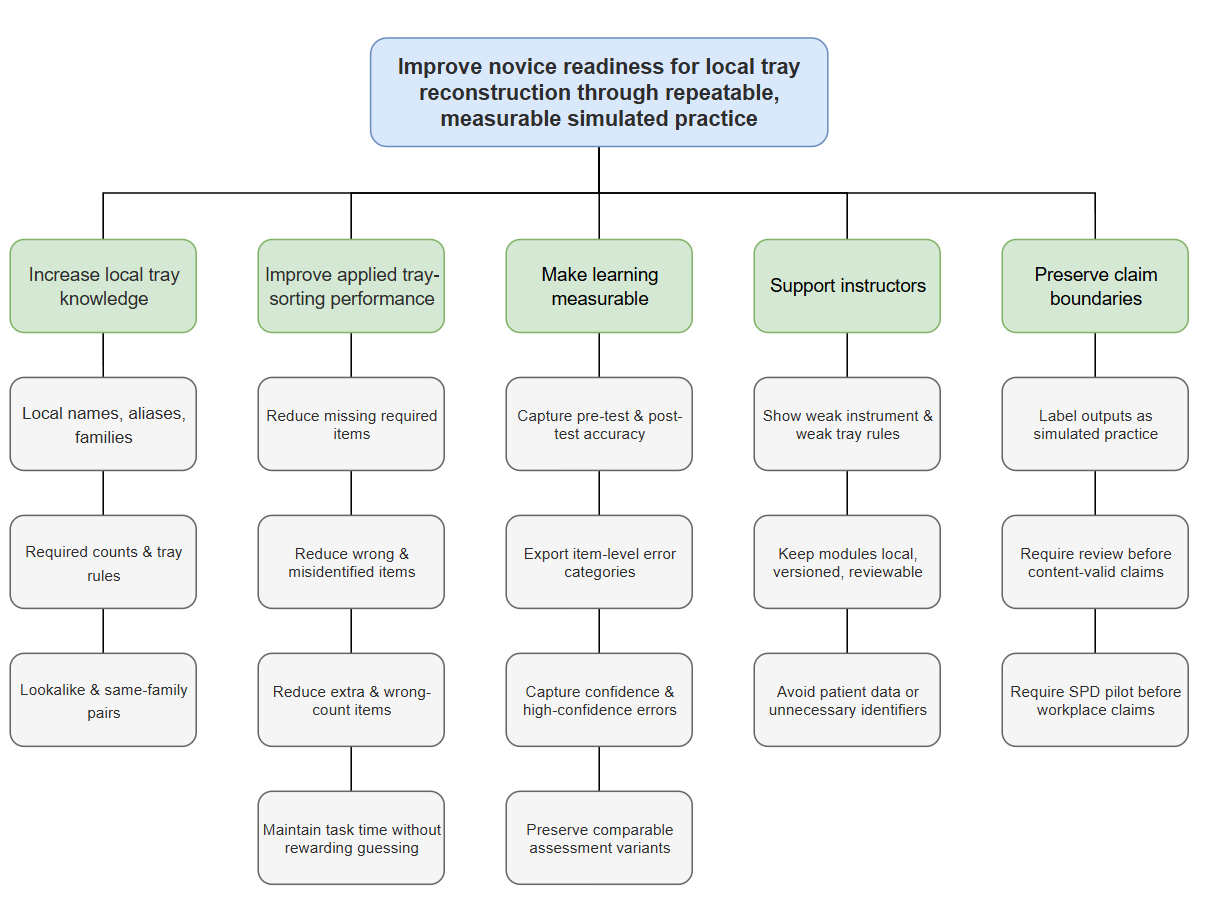
\includegraphics[width=0.85\textwidth]{figures/objective_tree.png}
\caption{Objective tree for TrayGuard's training intervention.}
\label{fig:objective-tree}
\end{figure}
\subsection{Performance Specifications}
\label{sec:performance-specifications}

The first build should use the following targets. They are deliberately
formative rather than clinical: they define when the prototype is ready to
support a project training-effectiveness claim.
\begin{table}[H]
\centering
\caption{Performance specifications and acceptance targets}
\label{tab:performance-specifications-and-acceptance-targets}
\small\renewcommand{\arraystretch}{1.2}\setlength{\tabcolsep}{4pt}
\begin{tabularx}{\textwidth}{|>{\raggedright\arraybackslash}X|>{\raggedright\arraybackslash}X|>{\raggedright\arraybackslash}X|>{\raggedright\arraybackslash}X|}
\hline
Area & Target & Evidence Basis & Measurement \\
\hline
Participant count & Minimum 8 baseline participants; target 12 complete participants if schedule allows. & NeuroVase used a 40-participant controlled study for an educational card/AR system, while qualitative methods literature supports small, narrow, homogeneous samples for early formative work \cite{jahani-et-al-2026-neurovase, malterud-et-al-2016, hennink-and-kaiser-2022}. & Unique participants with complete pre/post attempts. \\
\hline
Completion rate & At least 7 of 8 participants, or 85\% when n > 8, complete the full loop without blocking moderator intervention. & Usability must be separated from learning; NeuroVase used SUS and user-experience measures alongside knowledge testing. The System Usability Scale provides a standardized tool for assessing prototype usability in health-education contexts \cite{brooke-1996}. Additional measures such as the NASA Task Load Index \cite{nasa-tlx-accessed-2026} and established usability heuristics \cite{nielsen-norman-group-accessed-2026, porter-2003} could supplement formative evaluation. Health-specific usability scales offer clinically relevant assessment for future SPD pilots \cite{ghorayeb-et-al-2023}. & Completion flag and blocking help requests. \\
\hline
Accuracy gain & Mean paired tray accuracy improves by at least 20 percentage points from pre-test to post-test. & Ofstead's SP training pilot showed large pre/post score movement after structured teaching and hands-on practice; TrayGuard should set a smaller but visible formative threshold \cite{ofstead-et-al-2023}. & \texttt{post\_accuracy - pre\_accuracy}. \\
\hline
Post-test floor & Mean post-test accuracy is at least 80\%, and no more than one participant scores below 70\%. & The goal is not only improvement from a low baseline; learners should reach a usable simulated familiarity level before the module is considered ready. & Post-test \texttt{accuracy\_score}. \\
\hline
Severe-error reduction & Mean \texttt{missing + wrong + misidentified} errors decrease by at least 30\%. & Alfred et al. and Nichol et al. show missing, wrong, extra, and assembly-related errors are operationally meaningful categories \cite{alfred-et-al-2021, nichol-et-al-2024}. & Paired error-category counts. \\
\hline
Speed without unsafe guessing & Median post-test duration is at least 10\% lower, or is no more than 20\% higher if accuracy improves by at least 20 points. & Time matters because tray assembly is workflow-bound, but speed alone could reward guessing. & \texttt{duration\_seconds}, paired by learner. \\
\hline
Confidence calibration & High-confidence errors decline by at least 30\%; low-confidence correct answers are exported. & Ofstead captured confidence/satisfaction, and feedback research supports showing learners where they are and what to do next \cite{ofstead-et-al-2023, hattie-and-timperley-2007}. & Confidence >= 4 on incorrect items; confidence <= 2 on correct items. \\
\hline
Retention & A 7-day delayed tray sort retains at least half of the immediate accuracy gain and delayed accuracy does not return to within 5 percentage points of the pre-test baseline. & Bell et al. showed immediate medical-learning gains can decay within days and recommended reinforcement after as little as 1 week; same-day results should not be called retention \cite{bell-et-al-2008}. The 5pp falsification floor ensures retention is measured against baseline rather than as any positive number. & Delayed \texttt{accuracy\_score} relative to pre/post. \\
\hline
Convergent evidence & Post-test tray-sort accuracy correlates at r >= 0.50 with an independent photo-identification test of the same instruments administered in the same session. & Messick's external-aspect and Cook et al.'s relations-to-other-variables standard require that scores on the target task co-vary with a separate measure of the same construct \cite{messick-validity-1989, cook-beckman-validity-2006}. A photo-ID test shares the knowledge domain (instrument identity, aliases, lookalike discrimination) while differing in response format (identification without tray-sort context), so a moderate-to-strong correlation supports convergent validity. NeuroVase provides a recent precedent: Jahani et al. used independent knowledge tests alongside tangible-card simulation performance and found moderate correlations between measures \cite{jahani-et-al-2026-neurovase}. & Pearson r between post-test tray accuracy and photo-ID accuracy across participants. \\
\hline
Marker reliability & At least 95\% card detection in normal layouts and no systematic marker-ID confusion before user testing. & The marker layer is a measurement tool; if detection fails, scores confound learner error with app error. & Marker bench-test log. \\
\hline
Export completeness & Every completed run exports attempt-level and item-level records with required fields. & Instructor-facing evidence is part of the training value proposition. & CSV/JSON schema validation. \\
\hline
Demo success & A facilitator can load the module, run pre-test, study, quiz, practice sort, post-test, and export metrics in one uninterrupted demo. & The project requires an interactive demonstration of a functional design. & End-to-end checklist. \\
\hline
\end{tabularx}
\end{table}
\subsection{Quality Function Deployment}
\label{sec:quality-function-deployment}

Compact QFD:
\begin{table}[H]
\centering
\caption{Quality function deployment: needs to engineering targets}
\label{tab:quality-function-deployment-needs-to-engineering-targets}
\small\renewcommand{\arraystretch}{1.2}\setlength{\tabcolsep}{4pt}
\begin{tabularx}{\textwidth}{|>{\raggedright\arraybackslash}X|>{\raggedright\arraybackslash}X|>{\raggedright\arraybackslash}X|>{\raggedright\arraybackslash}X|}
\hline
Stakeholder need & Engineering characteristic & Target value & Verification \\
\hline
Learners can practice local tray content repeatedly. & File-backed module with required items, distractors, aliases, features, counts, and variants. & One complete \texttt{basic\_general\_tray\_v1} module with 8-12 required concepts and 3-6 distractors. & Module schema review and demo load. \\
\hline
Practice feels connected to tray reconstruction, not isolated memorization. & Simulated tray sort using physical cards or manual selection. & Pre-test, practice, post-test, and optional delayed variant all use the same tray rule. & End-to-end run. \\
\hline
Educators can see what learners missed. & Attempt-level and item-level export. & 100\% of completed runs export all required fields. & Schema validation. \\
\hline
Errors map to operationally meaningful categories. & Scoring engine with \texttt{missing}, \texttt{extra}, \texttt{wrong}, \texttt{misidentified}, and \texttt{wrong\_count}. & Every submitted tray receives category counts. & Unit tests or scored example cases. \\
\hline
Assessment is not contaminated by coaching. & Mode boundaries and feedback suppression. & No hints or corrective feedback in pre-test, post-test, or delayed modes. & UI walkthrough and export mode check. \\
\hline
The physical marker layer does not corrupt scores. & Marker reliability and user confirmation. & At least 95\% detection in normal layouts; confirmation before scoring. & Study 0 marker log. \\
\hline
Learner confidence is visible. & Confidence capture (1--5 scale). & High-confidence errors and low-confidence correct answers exported. & Export inspection. \\
\hline
The system remains ethical and nonpunitive. & Privacy and report labels. & Hashed learner IDs, no patient data, and report language that says practice evidence. & Report review. \\
\hline
Future teams can extend the design. & Versioned data model and traceability. & Module version, source notes, verification status, and assessment variant IDs included. & Data file review. \\
\hline
\end{tabularx}
\end{table}

\subsection{Function Analysis -- Transparent Box Model}
\label{sec:function-analysis-transparent-box-model}

The training system is modeled as a transparent box that transforms a local tray
module and physical instrument cards into learner performance evidence through
sequential subfunctions \cite{pahl-beitz-2007}:

\begin{table}[H]
\centering
\caption{Transparent box model for the training system}
\label{tab:transparent-box-model}
\small\renewcommand{\arraystretch}{1.2}\setlength{\tabcolsep}{4pt}
\begin{tabularx}{\textwidth}{|>{\raggedright\arraybackslash}X|>{\raggedright\arraybackslash}X|>{\raggedright\arraybackslash}X|}
\hline
Input & Subfunction & Output \\
\hline
Local tray module (JSON) & Authoring and verification & Verified tray template with required items, distractors, lookalike pairs, and assessment variants \\
\hline
Verified tray template & Pre-test assessment & Baseline accuracy, error-category counts, and confidence distribution \\
\hline
Instrument cards and tray template & Retrieval-first study & Prompt-before-reveal card practice with distinguishing features and aliases \\
\hline
Study session output & Identification quiz & Quiz accuracy, duration, and item-level confidence per instrument concept \\
\hline
Cards and tray template & Simulated tray sorting & Selected instrument set scored against required counts \\
\hline
Scored tray selection & Feedback generation & Missing, extra, wrong, misidentified, and wrong-count error report \\
\hline
Pre-test and post-test scores & Metrics aggregation & Pre/post accuracy gain, error reduction, confidence calibration, and weak-item report \\
\hline
Aggregated metrics & Export and reporting & CSV/JSON export with attempt-level and item-level records \\
\hline
\end{tabularx}
\end{table}

\subsection{Morphological Chart}
\label{sec:morphological-chart}

The morphological chart generates solution alternatives for each subfunction
identified in the transparent box model \cite{ulrich-et-al-2020, pahl-beitz-2007}.

\begin{table}[H]
\centering
\caption{Morphological chart: solution alternatives by subfunction}
\label{tab:morphological-chart}
\small\renewcommand{\arraystretch}{1.2}\setlength{\tabcolsep}{4pt}
\begin{tabularx}{\textwidth}{|>{\raggedright\arraybackslash}X|>{\raggedright\arraybackslash}X|>{\raggedright\arraybackslash}X|>{\raggedright\arraybackslash}X|>{\raggedright\arraybackslash}X|}
\hline
Subfunction & Alternative 1 & Alternative 2 & Alternative 3 & Alternative 4 \\
\hline
Content delivery & File-backed JSON module & Online database & Spreadsheet import & Hard-coded tray lists \\
\hline
Instrument representation & Physical marker cards & On-screen instrument icons & Real instruments & Text-based item list \\
\hline
Marker technology & AprilTag & QR code & ArUco & Manual selection \\
\hline
Learner interaction & Study + quiz + tray sort & Study-only & Quiz-only & Tray-sort only \\
\hline
Assessment mode & Pre/post with matched variants & Single post-test & Pre/post without variants & Continuous assessment \\
\hline
Feedback mechanism & Error-category report & Pass/fail only & Item-level hints & Instructor review only \\
\hline
Scoring approach & Category-based scoring (missing, extra, wrong, misidentified, wrong-count) & Simple accuracy (correct/total) & Weighted error severity & Confidence-adjusted scoring \\
\hline
Export format & CSV + JSON per run & Single PDF report & Instructor dashboard & Raw database access \\
\hline
\end{tabularx}
\end{table}

The selected combination is: file-backed JSON module, physical AprilTag marker
cards, full study-quiz-sort learning loop, pre/post matched-variant assessment,
category-based scoring, error-category feedback, and CSV/JSON export.

\subsection{Weighted Objective Method}
\label{sec:weighted-objective-method}

The weighted objective method scores each candidate solution combination against
weighted criteria derived from the objective tree and stakeholder needs \cite{ulrich-et-al-2020}.

\begin{table}[H]
\centering
\caption{Weighted objective method: solution path selection}
\label{tab:weighted-objective-method}
\small\renewcommand{\arraystretch}{1.2}\setlength{\tabcolsep}{4pt}
\begin{tabularx}{\textwidth}{|>{\raggedright\arraybackslash}X|>{\raggedright\arraybackslash}c|>{\raggedright\arraybackslash}c|>{\raggedright\arraybackslash}c|>{\raggedright\arraybackslash}c|>{\raggedright\arraybackslash}c|}
\hline
Criterion & Weight & Training path & CV tray checker & Software-only quiz & Real-instrument CV \\
\hline
Buildability within project scope & 0.25 & 5 & 1 & 4 & 1 \\
\hline
Measurable learning evidence & 0.20 & 5 & 2 & 3 & 3 \\
\hline
Physical task fidelity & 0.15 & 3 & 5 & 1 & 5 \\
\hline
Low validation burden & 0.15 & 4 & 1 & 4 & 1 \\
\hline
Instructor usefulness & 0.10 & 4 & 3 & 3 & 3 \\
\hline
Future extensibility & 0.10 & 3 & 4 & 2 & 4 \\
\hline
Cost and equipment requirements & 0.05 & 5 & 3 & 5 & 2 \\
\hline
Weighted total & 1.00 & 4.35 & 2.40 & 3.15 & 2.60 \\
\hline
\end{tabularx}
\end{table}

The training path scores highest (4.35/5.00), driven by buildability, measurable
evidence, and low validation burden.

\subsection{Requirement Traceability Matrix}


\begin{table}[H]
\centering
\caption{Requirement traceability matrix}
\label{tab:requirement-traceability-matrix}
\small\renewcommand{\arraystretch}{1.15}\setlength{\tabcolsep}{3pt}
\begin{tabularx}{\textwidth}{|>{\raggedright\arraybackslash}p{1.5cm}|>{\raggedright\arraybackslash}X|>{\raggedright\arraybackslash}X|>{\raggedright\arraybackslash}p{2.5cm}|>{\raggedright\arraybackslash}p{2.3cm}|>{\raggedright\arraybackslash}p{1.7cm}|}
\hline
Req. & Stakeholder need & Design feature & Evidence source & Validation method & Status \\
\hline
FR-1 Load local module & Educators need updateable local tray rules. & JSON tray module and module selector. & Count-sheet and local tray evidence \cite{nadeau-2024}. & Change module data and reload. & Ready for impl. \\
\hline
FR-2 Retrieval cards & Learners need active recall of names, features, and counts. & Prompt-before-reveal cards. & Retrieval and flashcard evidence \cite{roediger-and-karpicke-2006, barrison-et-al-2025}. & Card walkthrough and quiz logs. & Ready for impl. \\
\hline
FR-3 Pre/post assessment & Reviewers need measurable learning evidence. & No-hints pre-test and post-test variants. & Ofstead pre/post pattern \cite{ofstead-et-al-2023}. & Paired run export. & Protocol-ready. \\
\hline
FR-4 Quiz mode & Learners need feedback before applied sorting. & Quiz with confidence and weak-item logging. & Feedback and retrieval evidence \cite{hattie-and-timperley-2007}. & Quiz result export. & Ready for impl. \\
\hline
FR-5 Practice feedback & Learners need actionable correction. & Error-specific feedback engine. & Tray defect categories \cite{alfred-et-al-2021, nichol-et-al-2024}. & Seeded error cases. & Defined. \\
\hline
FR-6 Metrics export & Instructors need reviewable evidence. & Attempt and item CSV/JSON. & Error-reporting and competency evidence \cite{nichol-et-al-2024, ofstead-et-al-2023}. & Schema validation. & Defined. \\
\hline
FR-7 Mode separation & Assessment must remain fair. & Mode state and feedback suppression. & Assessment design and answer-leakage risk. & UI walkthrough. & Defined. \\
\hline
NFR-1 Fast data load & Demo cannot stall. & Local file storage. & Usability expectations. & Load timing <= 2 seconds. & Future test. \\
\hline
NFR-2 Short flow & Participants can finish in one session. & Bounded module and timed segments. & Study protocol and sample feasibility. & Timing <= 20 min for demo. & Future test. \\
\hline
NFR-3 Export reliability & No completed run should be lost. & Local export after each run. & Study evidence requirement. & 100\% completed-run exports. & Future test. \\
\hline
NFR-4 Privacy & Learners should not be surveilled unnecessarily. & Hashed IDs and no PHI. & Healthcare data governance concerns. & Export review. & Defined. \\
\hline
NFR-5 Content traceability & Local content must be auditable. & Source notes and instructor verification status. & Count-sheet and local content boundary. & Module review. & Defined. \\
\hline
NFR-6 Capability labels & Stakeholders must not overread scores. & Report language: simulated practice evidence. & Certification and clinical-transfer boundaries. & Report review. & Defined. \\
\hline
NFR-7 Accessibility & The interface must be usable by learners with varying abilities. & Audio controls, status messages, and color-independent indicators follow WCAG guidelines \cite{w3c-wai-audio-control-accessed-2026, w3c-wai-status-messages-accessed-2026, w3c-wai-use-of-color-accessed-2026}. & Accessibility audit and user testing. & Design review. & Future test. \\
\hline
\end{tabularx}
\end{table}

% ── Section 6 ──

\section{Final Product Concept And Design Rationale \hfill {\normalfont\small (Matthew, Andy, Qiyu)}}
\label{sec:final-product-concept-and-design-rationale}
\subsection{Final Product Concept}


TrayGuard is a local tray training and assessment platform. The core product is
a learner-facing app plus a file-backed tray module that defines the
instruments, aliases, required counts, distractors, lookalike pairs,
distinguishing features, and assessment variants for one local tray.
The first build should use printable AprilTag instrument cards as the physical
simulation layer. Each card represents one instrument or instrument variant.
The app scans the cards on a tabletop or tray area, treats the detected markers
as the learner's tray selection, scores the result against the tray template,
and returns missing, extra, wrong, misidentified, and wrong-count feedback in
practice mode. Pre-test and post-test modes suppress hints and corrective
feedback so the same system can collect baseline and post-training evidence.
The full learning loop is:
\begin{lstlisting}
local tray module -> pre-test -> retrieval-first cards -> quiz -> AprilTag-card tray sort -> post-test -> metrics export
\end{lstlisting}
This concept keeps the prototype buildable while preserving the task
structure: the learner must use local names, local counts, visual/semantic
distinctions, and tray rules to assemble a simulated tray.

\subsection{Alternatives Considered}


Several product directions were considered:
\begin{table}[H]
\centering
\caption{Alternative product directions considered and rejected}
\label{tab:alternative-product-directions-considered-and-rejected}
\small\renewcommand{\arraystretch}{1.2}\setlength{\tabcolsep}{4pt}
\begin{tabularx}{\textwidth}{|>{\raggedright\arraybackslash}X|>{\raggedright\arraybackslash}X|>{\raggedright\arraybackslash}X|}
\hline
Alternative & Benefit & Reason rejected or deferred \\
\hline
Deployment-grade CV tray checker on real instruments & Closest to the original automation concept and strongest if validated in an SPD. & Requires local instrument data, clinical workflow integration, failure-mode validation, and regulatory/adoption work beyond our project timeline. \\
\hline
Software-only study and quiz module & Fastest implementation path and easiest baseline study. & Too far from the tray reconstruction task; it would mostly test recognition, not applied count-sheet use. \\
\hline
Real teaching instruments with camera-supported tray review & Better physical fidelity than cards. & Requires access to representative instruments, cleaning/handling rules, storage, and educator review; appropriate for an SPD pilot after the simulated loop works. \\
\hline
Printable QR/AprilTag instrument cards & Cheap, portable, repeatable, and compatible with device scanning; closely matches NeuroVase-style tangible cue-card learning. & Less physically realistic than real instruments, so claims must stay limited to simulated tray-task improvement. \\
\hline
Manual drag-and-drop tray simulation & Simple software implementation without camera setup. & Does not exercise physical search, placement, or scanning workflow, and is less persuasive for an interactive project demo. \\
\hline
\end{tabularx}
\end{table}
The selected first prototype is the printable AprilTag-card path because it
creates a physical, measurable simulation without depending on deployment-grade
instrument recognition.
\subsection{Selected Candidate and Backup Paths}


The selected candidate is:
\begin{quote}
A local tray training and assessment app that uses printable AprilTag
instrument cards for simulated tray sorting, retrieval-first study, quiz,
practice feedback, no-hints pre/post assessment, and metrics export.
\end{quote}
The backup paths are layered so the project still produces evidence if one
piece fails.
\begin{table}[H]
\centering
\caption{Backup path strategy by risk level}
\label{tab:backup-path-strategy-by-risk-level}
\small\renewcommand{\arraystretch}{1.2}\setlength{\tabcolsep}{4pt}
\begin{tabularx}{\textwidth}{|>{\raggedright\arraybackslash}X|>{\raggedright\arraybackslash}X|>{\raggedright\arraybackslash}X|>{\raggedright\arraybackslash}X|}
\hline
Level & Selected path & Backup path & Claim preserved \\
\hline
Learning feature & Retrieval cards, quiz, practice sort, pre/post sort. & If the full loop is too long, run pre-test, study cards, practice sort, and post-test only. & Immediate simulated learning. \\
\hline
Physical interface & AprilTag cards scanned on a tray mat. & Use QR codes or manual card selection if AprilTag scanning is unreliable. & Local tray-task learning, with marker reliability reported as a limitation. \\
\hline
Content & \texttt{basic\_general\_tray\_v1} with 8-12 required concepts, distractors, lookalikes, and matched variants. & Reduce to 6-8 required concepts while preserving at least two lookalike pairs and count errors. & Bounded module feasibility. \\
\hline
CV & Marker detection only for project scoring. & Defer all camera recognition and score user selections manually. & Training evidence without CV overclaim. \\
\hline
Evaluation & 8-12 baseline participants plus delayed retention if schedule allows. & Run a smaller formative walkthrough and report it as usability/protocol evidence, not learning proof. & Risk-reduction handoff. \\
\hline
Content validity & SPD educator or instructor review. & Faculty or surgical-technology reviewer plus explicit future SPD review requirement. & Plausibility review, not clinical validation. \\
\hline
\end{tabularx}
\end{table}



\subsection{Rationale for AprilTag Marker Choice}

The prototype uses printable AprilTag fiducial markers on physical instrument
cards. This section justifies AprilTag specifically against the alternatives of
no physical component, QR codes, ArUco markers, and real instruments with
camera-based recognition.
\subsubsection{Why Physical Markers at All}

A purely digital drag-and-drop tray simulation would be simpler to implement
and would avoid camera-setup and detection-reliability concerns. It is rejected
because the target task is physical: SPD technicians search for,
pick up, examine, count, and arrange real instruments under a tray boundary
\cite{nichol-et-al-2024, alfred-et-al-2021}. A purely on-screen
interface removes the spatial search, the need to distinguish similar objects
in hand, and the physical count-and-place workflow that the study is meant to
simulate. Physical cards preserve those cognitive demands while replacing
regulated stainless-steel instruments with safe, cheap, tractable tokens.
\subsubsection{Why AprilTag over QR Codes, ArUco, or Real Instruments}

AprilTag was chosen over QR codes, ArUco markers, and real instruments for
reasons of detection robustness, error correction, and study feasibility.
Compared with QR codes, AprilTag provides faster corner detection at sub-pixel
precision, a lexicode-based Hamming-distance guarantee that corrects bit errors
from glare or occlusion, and native pose estimation for future spatial feedback
\cite{olson-2011, kalaitzakis-et-al-2021}.
Compared with ArUco, AprilTag's lexicode dictionary guarantees a larger minimum
inter-marker distance, and its corner-refinement pipeline produces more stable
localization across lighting and image scales
\cite{wang-et-al-2016-apriltag, garrido-jurado-et-al-2014, romero-ramirez-et-al-2018}. Compared with
real instruments --- the closest alternative to the original CV-checker goal ---
physical cards avoid the regulatory, handling, and recognition burdens that
would dominate the engineering schedule, and follow the same abstraction
strategy as NeuroVase's tangible cue cards
\cite{jahani-et-al-2026-neurovase, kienle-et-al-2025}. The recommended tag
family is \texttt{tagStandard52h13} (52 data bits, minimum Hamming distance 13),
supported through OpenCV's \texttt{aruco} module with no additional library dependency
\cite{krogius-et-al-2019, opencv-aruco-detection-accessed-2026}.
\subsection{Rationale for Gamified and Simulation-Based Learning Style}

TrayGuard embeds retrieval practice, feedback, scoring, progressive difficulty,
and confidence capture within a structured learning session. Each design
element maps to an established mechanism (summarized in
Section~\ref{sec:literature-and-related-work}): pre-testing improves later retention,
retrieval cards exercise active recall, weak-item logging enables targeted
remediation, error-category feedback supports deliberate practice, and
parallel no-hints post-tests prevent score inflation from layout memorization
\cite{cook-et-al-2011, roediger-and-karpicke-2006, hattie-and-timperley-2007, issenberg-et-al-2005, bell-et-al-2008}.

The design deliberately avoids leaderboards, badges, and competitive
ranking, which can shift motivation from intrinsic learning to extrinsic
reward-seeking \cite{van-gaalen-et-al-2021}.
Full VR simulation (e.g., SteriBoost) and narrative-driven modules (e.g.,
Touch Surgery) were considered but rejected because they add hardware or
authoring burden without increasing the number of tray-repetition cycles per
session
\cite{steriboost-accessed-2026, tulipan-et-al-2019}.
The chosen level is closest to the serious-game approach of SteriDefi---a
question-bank and scoring system that motivates repeated knowledge retrieval
\cite{vanhaverbeke-et-al-2018}.

\subsection{Training Session Walkthrough}
\label{sec:training-session-walkthrough}

Whereas the transparent box model
(Section~\ref{sec:function-analysis-transparent-box-model}) decomposed the
training flow into technical subfunctions, the following walkthrough
describes the same session from the learner's perspective.

The learner sits at a table with a printed count sheet, a pool of
AprilTag instrument cards face up, and a camera-connected device running
the TrayGuard app. The session proceeds through eight steps.

\textbf{Intake.}
The app displays a consent form and a brief background questionnaire
(prior SPD experience, certification status, familiarity with surgical
instrument trays). After submission, the app seeds a random assessment
variant and displays a prompt: ``Assemble the tray shown on the count
sheet using the cards in front of you.''

\textbf{Pre-test.}
The app enters assessment mode: no hints, no corrective feedback, no
timer visible to the learner but duration logged internally. The learner
places cards one at a time on a marked tray area. The camera detects
each card's AprilTag, maps it to an instrument ID, and adds it to the
running selection. The learner presses Confirm when finished. The
scoring engine classifies each required item as correct, missing, extra,
wrong, or misidentified, and each correct item as correct-count or
wrong-count. The accuracy score, error breakdown, and per-item
confidence are recorded but not shown.

\textbf{Retrieval-first study cards.}
The app switches to study mode. For each instrument in the tray module,
it shows a prompt card: the instrument name, image, aliases,
distinguishing features, and required quantity. The learner taps or
clicks to reveal the answer side with full details. The app records
which prompts the learner could not answer before revealing.

\textbf{Quiz.}
The app presents identification questions drawn from the same instrument
set. Each question shows an instrument image or name and asks for the
corresponding name, aliases, features, or count. After answering, the
learner rates confidence (1--5). The app records
correctness, confidence, and response time per item and flags weak items
(wrong or low-confidence answers).

\textbf{Practice tray sort.}
The learner repeats the same physical card-sorting task as the pre-test.
This time, the app provides immediate feedback: after each card is
placed, it indicates whether the item is correct, wrong (wrong
instrument placed), or extra (not on the tray list). After Confirm, the
app shows the full error-category breakdown with correct, missing,
extra, wrong, misidentified, and wrong-count counts, and highlights
each error in the tray visualization.

\textbf{Weak-item review.}
If the study protocol includes this step, the app redisplays retrieval
cards for items the learner missed or answered with low confidence
during the quiz or practice sort, allowing focused re-study before the
post-test.

\textbf{Post-test.}
The app switches back to assessment mode with a parallel tray variant
(different instrument subset, same lookalike pairs, matched difficulty).
The procedure matches the pre-test: no hints, no feedback, timed but no
visible timer. The learner sorts cards and confirms. The scoring engine
records the same metrics for pre/post comparison.

\textbf{Summary and export.}
The app displays a session summary: pre-test and post-test accuracy
scores, error-category counts side by side, confidence calibration
(high-confidence errors, low-confidence correct answers), and a list of
weak items that did not improve. The instructor or facilitator receives
a CSV/JSON export with attempt-level and item-level records, hashed
learner ID, module version, and assessment variant IDs.





% ── Section 7 ──

\section{System Design \hfill {\normalfont\small (Matthew, Jacob)}}
\label{sec:system-design}
\subsection{System Overview}


TrayGuard should be built as a local module runner plus a card-scanning
assessment surface. The app recognizes simulated instrument cards for the
first study. It observes which cards the learner placed in the tray area, scores
that selection against a local tray template, and exports evidence.
The architecture follows the evidence base:
\begin{itemize}
  \item Local tray modules are required because count sheets define tray names, contents, quantities, sizes, and reference/catalog numbers, and real count sheets include fields such as reference number, description, location, quantity, check box, total count, and hospital signature \cite{nadeau-2024, stryker-gamma4-count-sheet-2023, stryker-imn-count-sheet-2023}.
  \item Retrieval-first study and quiz modes are justified by retrieval practice, health-professions flashcard evidence, and spaced digital education \cite{roediger-and-karpicke-2006, barrison-et-al-2025, martinengo-et-al-2024}.
  \item Pre/post practice, confidence capture, and optional delayed retention follow the sterile-processing precedent in Ofstead and the retention warning in Bell et al. \cite{ofstead-et-al-2023, bell-et-al-2008}.
   \item AprilTag cards are a physical proxy for instrument selection and counting decisions. The tangible-card idea is supported by NeuroVase-style cue cards and board/card-based healthcare education, but clinical transfer remains future validation \cite{jahani-et-al-2026-neurovase, ward-et-al-2019}.
\end{itemize}
\subsection{Subsystem Breakdown}


The system separates into these functional subsystems:
\begin{table}[H]
\centering
\caption{Functional subsystem breakdown}
\label{tab:functional-subsystem-breakdown}
\small\renewcommand{\arraystretch}{1.2}\setlength{\tabcolsep}{4pt}
\begin{tabularx}{\textwidth}{|>{\raggedright\arraybackslash}X|>{\raggedright\arraybackslash}X|}
\hline
Subsystem & Responsibility \\
\hline
Local content/tray module & Stores instrument records, aliases, photos, distinguishing features, required quantities, distractors, and tray-template versions. \\
\hline
Learning workflow & Routes the learner through pre-test, study, quiz, practice sort, weak-item review, post-test, and export. \\
\hline
Retrieval practice & Presents prompt-before-answer cards and quizzes for instrument names, features, lookalikes, and required counts. \\
\hline
AprilTag card scanning & Detects printed marker cards and maps marker IDs to instrument IDs so the app can observe a physical tray simulation. \\
\hline
Simulated tray scoring & Compares detected cards and selected quantities against the tray template. \\
\hline
Feedback engine & Reports missing, extra, wrong, misidentified, and wrong-count errors in practice mode. \\
\hline
Confidence/uncertainty capture & Records confidence ratings (1--5 scale) for assessment and instructor review. \\
\hline
Reporting/export & Produces pre/post accuracy, time, error-category, confidence, and weak-item summaries. \\
\hline
Instructor review & Lets an educator verify tray content, local naming, distractors, and study evidence before broader use. \\
\hline
\end{tabularx}
\end{table}
Computer vision for recognizing real instruments remains a future support
subsystem. In the project build, the marker-scanning subsystem is a
proxy for observing user decisions.

\begin{figure}[H]
\centering
\caption{Functional block diagram. Please I really tried.}
\label{fig:functional-block-diagram}
\resizebox{\textwidth}{!}{%
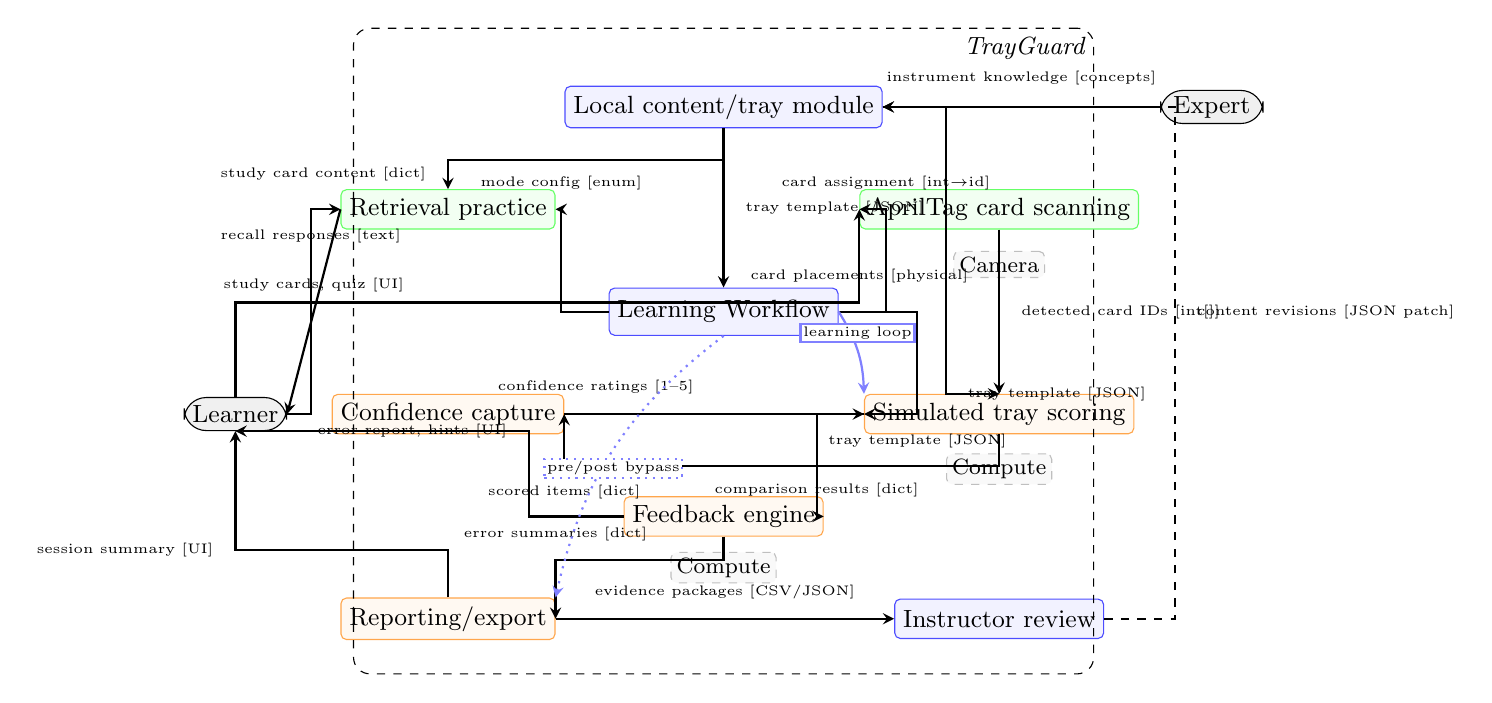
\begin{tikzpicture}[
    block/.style={rectangle, draw, rounded corners=2pt, minimum width=2.5cm, minimum height=0.5cm, align=center, font=\small, inner sep=3pt},
    external/.style={rectangle, draw, rounded corners=8pt, minimum width=1.3cm, minimum height=0.42cm, align=center, font=\small, fill=gray!12, inner sep=2pt},
    resource/.style={rectangle, draw=gray!50, dashed, rounded corners=2pt, minimum width=0.9cm, minimum height=0.28cm, align=center, font=\footnotesize, inner sep=2pt, fill=gray!5},
    arrow/.style={->, >=stealth, thick},
    returnarrow/.style={->, >=stealth, thick, dashed},
    every path/.style={font=\tiny}
]

% ─ Central hub ──
\node[block, fill=blue!5, draw=blue!70, minimum width=2.8cm, minimum height=0.6cm] (workflow) at (0,0) {Learning Workflow};

% ── Top row ──
\node[block, fill=blue!5, draw=blue!70] (content) at (0, 2.6) {Local content/tray module};

% ── Second row ──
\node[block, fill=green!5, draw=green!60] (retrieval) at (-3.5, 1.3) {Retrieval practice};
\node[block, fill=green!5, draw=green!60] (scanning) at (3.5, 1.3) {AprilTag card scanning};

% ── Third row ──
\node[block, fill=orange!5, draw=orange!70] (confidence) at (-3.5, -1.3) {Confidence capture};
\node[block, fill=orange!5, draw=orange!70] (scoring) at (3.5, -1.3) {Simulated tray scoring};

% ── Bottom row ─
\node[block, fill=orange!5, draw=orange!70] (feedback) at (0, -2.6) {Feedback engine};
\node[block, fill=orange!5, draw=orange!70] (reporting) at (-3.5, -3.9) {Reporting/export};
\node[block, fill=blue!5, draw=blue!70] (instructor) at (3.5, -3.9) {Instructor review};

% ─ Internal resource badges ──
\node[resource] (cam) at (3.5, 0.6) {Camera};
\node[resource] (comp1) at (3.5, -2.0) {Compute};
\node[resource] (comp2) at (0, -3.25) {Compute};

% ── System boundary ─
\node[draw, dashed, rounded corners=6pt, minimum width=9.4cm, minimum height=8.2cm] (boundary) at (0, -0.5) {};
\node[anchor=north east, font=\small\itshape] at (boundary.north east) {TrayGuard};

% ── External entities (outside boundary) ──
\node[external] (learner) at (-6.2, -1.3) {Learner};
\node[external] (expert) at (6.2, 2.6) {Expert};

% ═════════════════════════════════════════════════
% ARROWS — all orthogonal routing
% ══════════════════════════════════════════════════

% Expert → Content (horizontal)
\draw[arrow] (expert.west) -- (content.east)
  node[midway, above=0.15cm, font=\tiny] {instrument knowledge [concepts]};

% Content → Workflow (vertical)
\draw[arrow] (content.south) -- (workflow.north)
  node[midway, right=0.15cm, font=\tiny] {tray template [JSON]};

% Content → Retrieval (down-left, orthogonal)
\draw[arrow] (content.south) -- ++(0,-0.4) -| (retrieval.north)
  node[pos=0.75, left=0.15cm, font=\tiny] {study card content [dict]};

% Content → Scoring (down-right, orthogonal, wide route)
\draw[arrow] (content.east) -- ++(0.8,0) |- (scoring.north)
  node[pos=0.5, right=0.15cm, font=\tiny] {tray template [JSON]};

% Workflow → Retrieval (left)
\draw[arrow] (workflow.west) -- ++(-0.6,0) |- (retrieval.east)
  node[pos=0.5, above=0.12cm, font=\tiny] {mode config [enum]};

% Workflow → Scanning (right)
\draw[arrow] (workflow.east) -- ++(0.6,0) |- (scanning.west)
  node[pos=0.5, above=0.12cm, font=\tiny] {card assignment [int$\to$id]};

% Workflow → Scoring (down-right, below scanning route)
\draw[arrow] (workflow.east) -- ++(1.0,0) |- (scoring.west)
  node[pos=0.5, below=0.12cm, font=\tiny] {tray template [JSON]};

% Retrieval → Learner (left)
\draw[arrow] (retrieval.west) -- (learner.east)
  node[midway, above=0.12cm, font=\tiny] {study cards, quiz [UI]};

% Learner → Retrieval (left, below)
\draw[arrow] (learner.east) -- ++(0.3,0) |- (retrieval.west)
  node[pos=0.5, below=0.12cm, font=\tiny] {recall responses [text]};

% Learner → Scanning (up-right, orthogonal)
\draw[arrow] (learner.north) -- ++(0,1.2) -| (scanning.west)
  node[pos=0.5, above=0.12cm, font=\tiny] {card placements [physical]};

% Scanning → Scoring (vertical)
\draw[arrow] (scanning.south) -- (scoring.north)
  node[midway, right=0.15cm, font=\tiny] {detected card IDs [int[]]};

% Scoring → Feedback (left)
\draw[arrow] (scoring.west) -- ++(-0.6,0) |- (feedback.east)
  node[pos=0.5, above=0.12cm, font=\tiny] {comparison results [dict]};

% Scoring → Confidence (left, routed below)
\draw[arrow] (scoring.south) -- ++(0,-0.4) -| (confidence.east)
  node[pos=0.5, below=0.12cm, font=\tiny] {scored items [dict]};

% Confidence → Scoring (right, routed above)
\draw[arrow] (confidence.east) -- ++(0.4,0) |- (scoring.west)
  node[pos=0.5, above=0.12cm, font=\tiny] {confidence ratings [1--5]};

% Feedback → Learner (left-up, orthogonal)
\draw[arrow] (feedback.west) -- ++(-1.2,0) |- (learner.south)
  node[pos=0.5, left=0.15cm, font=\tiny] {error report, hints [UI]};

% Feedback → Reporting (down-left)
\draw[arrow] (feedback.south) -- ++(0,-0.3) -| (reporting.east)
  node[pos=0.5, above=0.12cm, font=\tiny] {error summaries [dict]};

% Reporting → Learner (up)
\draw[arrow] (reporting.north) -- ++(0,0.6) -| (learner.south)
  node[pos=0.5, left=0.15cm, font=\tiny] {session summary [UI]};

% Reporting → Instructor (right, along bottom)
\draw[arrow] (reporting.east) -- (instructor.west)
  node[midway, above=0.12cm, font=\tiny] {evidence packages [CSV/JSON]};

% Instructor → Content (dashed feedback loop, routed right side)
\draw[returnarrow] (instructor.east) -- ++(0.9,0) |- (content.east)
  node[pos=0.3, right=0.15cm, font=\tiny] {content revisions [JSON patch]};

% Learning loop annotation
\draw[arrow, draw=blue!50, bend left=15] (workflow.east) to
  node[above=0.1cm, font=\tiny, draw=blue!50, fill=white, inner sep=1pt] {learning loop} (scoring.north west);

% Pre/post bypass annotation
\draw[arrow, draw=blue!50, dotted, bend right=20] (workflow.south) to
  node[below=0.1cm, font=\tiny, draw=blue!50, fill=white, inner sep=1pt] {pre/post bypass} (reporting.north east);

\end{tikzpicture}%
}
\end{figure}

\begin{figure}[H]
\centering
\caption{Dependency diagram. Please I really tried.}
\label{fig:dependency-diagram}
\resizebox{\textwidth}{!}{%
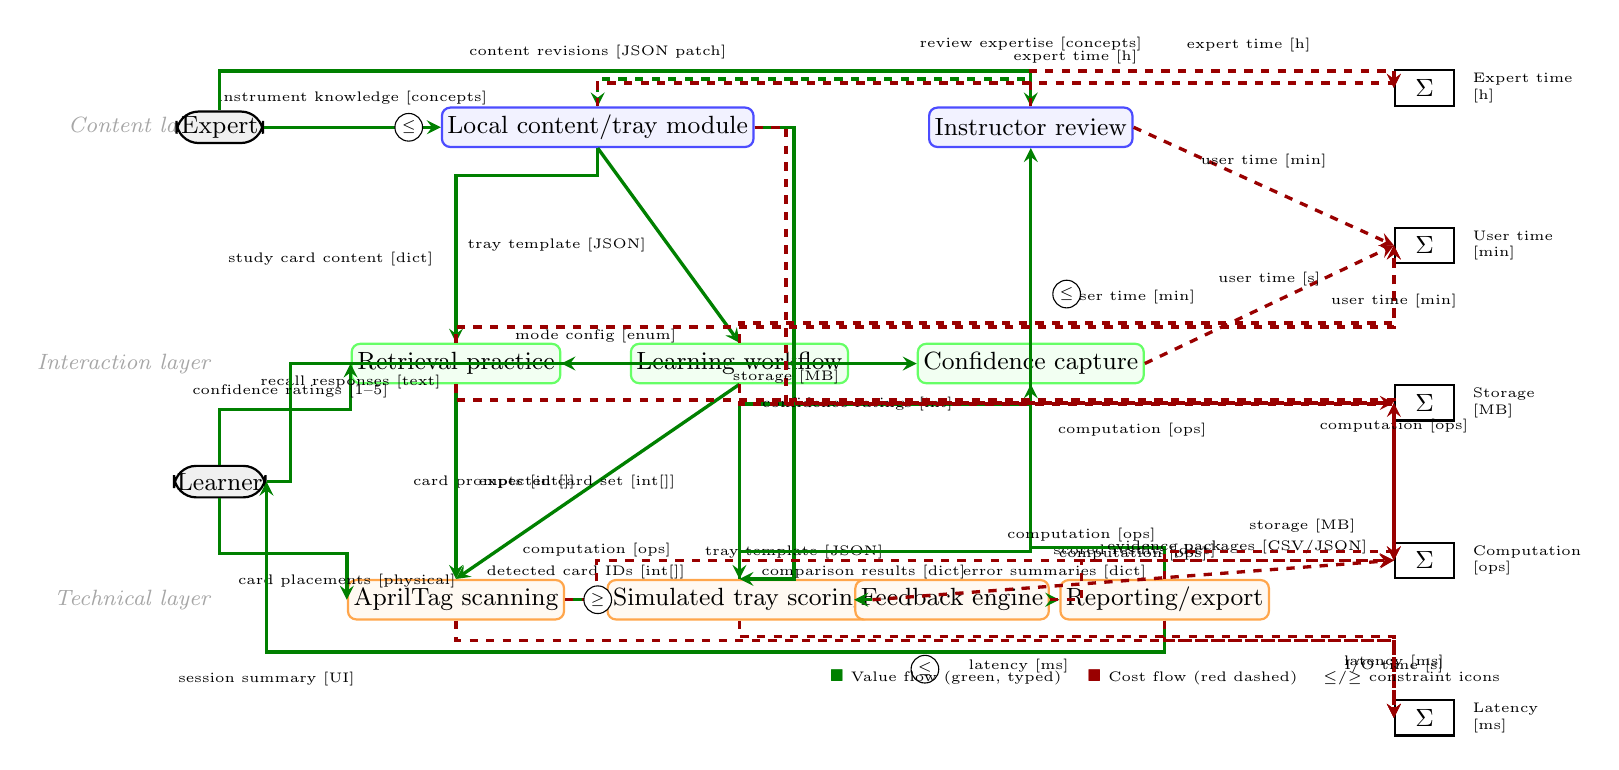
\begin{tikzpicture}[
    block/.style={rectangle, draw, thick, rounded corners=3pt, minimum width=2.2cm, minimum height=0.5cm, align=center, font=\small, inner sep=2pt},
    external/.style={rectangle, draw, thick, rounded corners=8pt, minimum width=1.1cm, minimum height=0.4cm, align=center, font=\small, fill=gray!12, inner sep=1pt},
    aggregator/.style={rectangle, draw, thick, minimum width=0.75cm, minimum height=0.45cm, align=center, font=\small, inner sep=2pt},
    layerlabel/.style={font=\footnotesize\itshape, text=gray!70, anchor=east},
    valuearrow/.style={->, >=stealth, very thick, draw=green!50!black},
    costarrow/.style={->, >=stealth, very thick, draw=red!60!black, dashed},
    every path/.style={font=\tiny},
    constraint/.style={draw, circle, fill=white, inner sep=1pt, font=\tiny}
]

% ══════════════════════════════════════════════════
% LAYER LABELS (far left, outside flow area)
% ══════════════════════════════════════════════════
\node[layerlabel] at (-4.8, 3.0) {Content layer};
\node[layerlabel] at (-4.8, 0.0) {Interaction layer};
\node[layerlabel] at (-4.8, -3.0) {Technical layer};

% ══════════════════════════════════════════════════
% CONTENT LAYER (y = 3.0)
% ══════════════════════════════════════════════════
\node[block, fill=blue!5, draw=blue!70] (content) at (0, 3.0) {Local content/tray module};
\node[block, fill=blue!5, draw=blue!70] (instructor) at (5.5, 3.0) {Instructor review};

% ══════════════════════════════════════════════════
% INTERACTION LAYER (y = 0.0)
% ══════════════════════════════════════════════════
\node[block, fill=green!5, draw=green!60] (retrieval) at (-1.8, 0.0) {Retrieval practice};
\node[block, fill=green!5, draw=green!60] (workflow) at (1.8, 0.0) {Learning workflow};
\node[block, fill=green!5, draw=green!60] (confidence) at (5.5, 0.0) {Confidence capture};

% ══════════════════════════════════════════════════
% TECHNICAL LAYER (y = -3.0)
% ══════════════════════════════════════════════════
\node[block, fill=orange!5, draw=orange!70] (scanning) at (-1.8, -3.0) {AprilTag scanning};
\node[block, fill=orange!5, draw=orange!70] (scoring) at (1.8, -3.0) {Simulated tray scoring};
\node[block, fill=orange!5, draw=orange!70] (feedback) at (4.5, -3.0) {Feedback engine};
\node[block, fill=orange!5, draw=orange!70] (reporting) at (7.2, -3.0) {Reporting/export};

% ══════════════════════════════════════════════════
% EXTERNAL ENTITIES (far left)
% ══════════════════════════════════════════════════
\node[external] (expert) at (-4.8, 3.0) {Expert};
\node[external] (learner) at (-4.8, -1.5) {Learner};

% ══════════════════════════════════════════════════
% COST AGGREGATORS (far right, staggered vertically)
% ══════════════════════════════════════════════════
\node[aggregator] (sum_expert) at (10.5, 3.5) {$\Sigma$};
\node[right=0.1cm of sum_expert, font=\tiny, align=left] {Expert time\\{[}h{]}};

\node[aggregator] (sum_user) at (10.5, 1.5) {$\Sigma$};
\node[right=0.1cm of sum_user, font=\tiny, align=left] {User time\\{[}min{]}};

\node[aggregator] (sum_storage) at (10.5, -0.5) {$\Sigma$};
\node[right=0.1cm of sum_storage, font=\tiny, align=left] {Storage\\{[}MB{]}};

\node[aggregator] (sum_compute) at (10.5, -2.5) {$\Sigma$};
\node[right=0.1cm of sum_compute, font=\tiny, align=left] {Computation\\{[}ops{]}};

\node[aggregator] (sum_latency) at (10.5, -4.5) {$\Sigma$};
\node[right=0.1cm of sum_latency, font=\tiny, align=left] {Latency\\{[}ms{]}};

% ══════════════════════════════════════════════════
% VALUE ARROWS (green solid) — orthogonal routing
% All routed in the center area between blocks
% ══════════════════════════════════════════════════

% Expert → Content (horizontal)
\draw[valuearrow] (expert) -- (content)
  node[midway, above=0.15cm, font=\tiny] {instrument knowledge [concepts]};

% Expert → Instructor (routed above content layer)
\draw[valuearrow] (expert.north) -- ++(0,0.5) -| (instructor.north)
  node[pos=0.5, above=0.12cm, font=\tiny] {review expertise [concepts]};

% Learner → Retrieval (up-right, orthogonal)
\draw[valuearrow] (learner.north) -- ++(0,0.7) -| (retrieval.west)
  node[pos=0.5, above=0.12cm, font=\tiny] {recall responses [text]};

% Learner → Scanning (down-right, orthogonal)
\draw[valuearrow] (learner.south) -- ++(0,-0.7) -| (scanning.west)
  node[pos=0.5, below=0.12cm, font=\tiny] {card placements [physical]};

% Learner → Confidence (right, orthogonal)
\draw[valuearrow] (learner.east) -- ++(0.3,0) |- (confidence.west)
  node[pos=0.5, below=0.12cm, font=\tiny] {confidence ratings [1--5]};

% Content → Workflow (vertical)
\draw[valuearrow] (content.south) -- (workflow.north)
  node[midway, left=0.15cm, font=\tiny] {tray template [JSON]};

% Content → Retrieval (down-left, orthogonal)
\draw[valuearrow] (content.south) -- ++(0,-0.35) -| (retrieval.north)
  node[pos=0.75, left=0.15cm, font=\tiny] {study card content [dict]};

% Content → Scoring (down-right, orthogonal, wide route)
\draw[valuearrow] (content.east) -- ++(0.5,0) |- (scoring.north)
  node[pos=0.5, above=0.12cm, font=\tiny] {tray template [JSON]};

% Workflow → Retrieval (left)
\draw[valuearrow] (workflow) -- (retrieval)
  node[midway, above=0.12cm, font=\tiny] {mode config [enum]};

% Workflow → Scanning (vertical)
\draw[valuearrow] (workflow.south) -- (scanning.north)
  node[midway, left=0.15cm, font=\tiny] {card prompts [int[]]};

% Retrieval → Scanning (vertical)
\draw[valuearrow] (retrieval.south) -- (scanning.north)
  node[midway, right=0.15cm, font=\tiny] {expected card set [int[]]};

% Scanning → Scoring (right)
\draw[valuearrow] (scanning) -- (scoring)
  node[midway, above=0.12cm, font=\tiny] {detected card IDs [int[]]};

% Scoring → Feedback (right)
\draw[valuearrow] (scoring) -- (feedback)
  node[midway, above=0.12cm, font=\tiny] {comparison results [dict]};

% Scoring → Confidence (up-right, orthogonal)
\draw[valuearrow] (scoring.north) -- ++(0,0.35) -| (confidence.south)
  node[pos=0.5, right=0.15cm, font=\tiny] {scored results [dict]};

% Confidence → Scoring (down-left, orthogonal, offset)
\draw[valuearrow] (confidence.south) -- ++(0,-0.25) -| (scoring.north)
  node[pos=0.5, right=0.15cm, font=\tiny] {confidence ratings [int]};

% Feedback → Reporting (right)
\draw[valuearrow] (feedback) -- (reporting)
  node[midway, above=0.12cm, font=\tiny] {error summaries [dict]};

% Reporting → Instructor (up, orthogonal)
\draw[valuearrow] (reporting.north) -- ++(0,0.4) -| (instructor.south)
  node[pos=0.3, right=0.15cm, font=\tiny] {evidence packages [CSV/JSON]};

% Reporting → Learner (left-up, orthogonal)
\draw[valuearrow] (reporting.south) -- ++(0,-0.4) -| (learner.east)
  node[pos=0.5, below=0.12cm, font=\tiny] {session summary [UI]};

% Instructor → Content (dashed feedback loop, routed above)
\draw[valuearrow, dashed] (instructor.north) -- ++(0,0.35) -| (content.north)
  node[pos=0.5, above=0.12cm, font=\tiny] {content revisions [JSON patch]};

% ══════════════════════════════════════════════════
% COST ARROWS (red dashed) — routed on the right periphery
% Each block emits a short horizontal stub, then routes
% vertically in the rightmost lane to its Σ aggregator.
% Upper/lower lane separation prevents overlap.
% ══════════════════════════════════════════════════

% ── Content layer costs ──
% Content → Σ Expert time (upper lane, above content layer)
\draw[costarrow] (content.north) -- ++(0,0.3) -| (sum_expert.west)
  node[pos=0.3, above=0.1cm, font=\tiny] {expert time [h]};

% Content → Σ Storage (middle lane)
\draw[costarrow] (content.east) -- ++(0.4,0) |- (sum_storage.west)
  node[pos=0.5, above=0.1cm, font=\tiny] {storage [MB]};

% Instructor → Σ Expert time (upper lane, right side)
\draw[costarrow] (instructor.north) -- ++(0,0.45) -| (sum_expert.west)
  node[pos=0.3, above=0.1cm, font=\tiny] {expert time [h]};

% Instructor → Σ User time (direct right)
\draw[costarrow] (instructor.east) -- (sum_user.west)
  node[midway, above=0.1cm, font=\tiny] {user time [min]};

% ── Interaction layer costs ──
% Workflow → Σ User time (upper lane)
\draw[costarrow] (workflow.north) -- ++(0,0.25) -| (sum_user.west)
  node[pos=0.3, above=0.1cm, font=\tiny] {user time [min]};

% Workflow → Σ Computation (lower lane)
\draw[costarrow] (workflow.south) -- ++(0,-0.25) -| (sum_compute.west)
  node[pos=0.3, below=0.1cm, font=\tiny] {computation [ops]};

% Retrieval → Σ User time (upper lane)
\draw[costarrow] (retrieval.north) -- ++(0,0.2) -| (sum_user.west)
  node[pos=0.5, above=0.1cm, font=\tiny] {user time [min]};

% Retrieval → Σ Computation (lower lane)
\draw[costarrow] (retrieval.south) -- ++(0,-0.2) -| (sum_compute.west)
  node[pos=0.5, below=0.1cm, font=\tiny] {computation [ops]};

% Confidence → Σ User time (direct right)
\draw[costarrow] (confidence.east) -- (sum_user.west)
  node[midway, above=0.1cm, font=\tiny] {user time [s]};

% ── Technical layer costs ──
% Scanning → Σ Computation (upper lane)
\draw[costarrow] (scanning.east) -- ++(0.4,0) |- (sum_compute.west)
  node[pos=0.3, above=0.1cm, font=\tiny] {computation [ops]};

% Scanning → Σ Latency (lower lane, below technical layer)
\draw[costarrow] (scanning.south) -- ++(0,-0.25) -| (sum_latency.west)
  node[pos=0.3, below=0.1cm, font=\tiny] {latency [ms]};

% Scoring → Σ Computation (direct right)
\draw[costarrow] (scoring.east) -- (sum_compute.west)
  node[midway, above=0.1cm, font=\tiny] {computation [ops]};

% Scoring → Σ Latency (lower lane)
\draw[costarrow] (scoring.south) -- ++(0,-0.2) -| (sum_latency.west)
  node[pos=0.5, below=0.1cm, font=\tiny] {latency [ms]};

% Feedback → Σ Computation (upper lane)
\draw[costarrow] (feedback.east) -- ++(0.4,0) |- (sum_compute.west)
  node[pos=0.5, above=0.1cm, font=\tiny] {computation [ops]};

% Reporting → Σ Storage (upper lane)
\draw[costarrow] (reporting.north) -- ++(0,0.35) -| (sum_storage.west)
  node[pos=0.3, above=0.1cm, font=\tiny] {storage [MB]};

% Reporting → Σ Latency (lower lane)
\draw[costarrow] (reporting.south) -- ++(0,-0.25) -| (sum_latency.west)
  node[pos=0.5, below=0.1cm, font=\tiny] {I/O time [s]};

% ══════════════════════════════════════════════════
% CONSTRAINT ICONS
% ══════════════════════════════════════════════════
\node[constraint] at ($(expert)!0.5!(content)$) {$\leq$};
\node[constraint] at ($(scanning)!0.5!(scoring)$) {$\geq$};
\node[constraint] at ($(workflow.north)!0.5!(sum_user.west)$) {$\leq$};
\node[constraint] at ($(scanning.south)!0.5!(sum_latency.west)$) {$\leq$};

% ══════════════════════════════════════════════════
% LEGEND
% ══════════════════════════════════════════════════
\node[below=0.5cm of reporting, anchor=north, font=\tiny, align=left]
  {\textcolor{green!50!black}{$\blacksquare$}~Value flow (green, typed) \quad
   \textcolor{red!60!black}{$\blacksquare$}~Cost flow (red dashed) \quad
   $\leq$/$\geq$~constraint icons};

\end{tikzpicture}%
}
\end{figure}

\subsection{Data Model and Module Contract}
\label{sec:data-model-and-module-contract}

The data model should mirror a real count sheet while staying small enough for
the first build. Stryker's public count sheets show the practical minimum:
reference number, description, location/layer, quantity, check box, total count,
additional items, and hospital signature. TrayGuard adds learning-specific
fields for aliases, lookalikes, confidence, and error categories.
The full data model specification is listed in Appendix~\ref{app:system-design-reference-tables}, Table~\ref{tab:app-data-model-objects}.
The table fields map real count-sheet columns (reference number, description, location, quantity) while adding learning-specific fields for aliases, lookalike pairs, and confidence capture. Required-item references are validated against instrument definitions, lookalike pairs must resolve to valid instrument IDs, and assessment variants must reference existing items. Every instrument carries \texttt{local\_verification\_status: "pending\_review"} until expert review (Study~3, Section~\ref{sec:evaluation-and-validation-plan}) validates the content.

The first implementation can store these objects in JSON files and export CSV
for analysis. The constraint is schema stability: pre-test, post-test,
and delayed retention must produce comparable rows. A sample instrument
record is shown in Appendix~\ref{app:sample-instrument-json}.
\subsection{Learning Loop}


The learning loop (Section~\ref{sec:final-product-concept-and-design-rationale}) applies retrieval practice as the instructional engine. The learner should usually
commit to an answer before the system reveals it: name the instrument, identify
a distinguishing feature, choose the lookalike, recall the count, or decide
whether the item belongs in the tray. The simulated tray sort is applied
retrieval: the learner must use those same facts in context with distractors
and quantities.

Each feature's evidence-based role and engineering requirement is catalogued in Appendix~\ref{app:system-design-reference-tables}, Table~\ref{tab:app-feature-to-evidence}.
\subsection{FGVC-Derived Module Plausibility}


The first module should contain:
\begin{itemize}
  \item 8-12 required instrument concepts;
  \item 3-6 distractor instruments;
  \item 2-4 known lookalike or same-family pairs;
  \item local names, aliases, family labels, required counts, and distinguishing features;
  \item AprilTag cards that represent instruments during the physical tray simulation;
  \item parallel pre-test, post-test, and delayed-retention tray variants with matched difficulty;
  \item instructor or expert review before results are presented as content-valid.
\end{itemize}
The cards should use neutral assessment fronts. Names, counts, and obvious
answer labels should be hidden during pre-test, post-test, and retention tasks
so the participant cannot solve the task by reading the card.

The FGVC-derived modules are practice modules built from the major-tray image
classes reported by Atabuzzaman et al. \cite{atabuzzaman-et-al-2025}. The
source contributes instrument names and images for a bounded image-card set:
scissors, clamps, forceps, needle holders, retractors, suction, and other
classes present in the major-tray archive. It gives TrayGuard a coherent pool of
real instrument classes photographed under one dataset program.

Plausibility for these modules comes from three linked sources of evidence.
First, every required card, distractor card, and lookalike pair is selected from
the FGVC major-tray class mapping. Second, the module schema mirrors real
tray/count-sheet fields: tray name, required item, quantity, reference number,
location or layer, total count, and check status
\cite{stryker-gamma4-count-sheet-2023, stryker-imn-count-sheet-2023}. The FGVC-derived quantities are simulated
as one card per selected class. The FGVC12 subset provides 16 instruments
across four families (cutting/dissecting, clamping/occluding, grasping/holding,
suturing), with six documented lookalike discriminations
(Table~\ref{tab:fgvc12-module-instruments}). Each instrument in the tray module
schema carries a \texttt{distinguishing\_features} array and participates in
\texttt{lookalike\_pairs} that encode clinical feedback messages at the pair
level:
\begin{itemize}
  \item Mayo curved vs Metzenbaum curved: ``Mayo scissors have heavier, broader blades; Metzenbaum are slimmer and lighter for delicate tissue.''
  \item Kelly vs Crile: ``Check serration pattern: Kelly serrations are distal half; Crile serrations run the full jaw.''
  \item Allis vs Babcock: ``Allis has multiple interlocking teeth; Babcock has smooth fenestrated jaws.''
  \item Adson vs DeBakey: ``Adson is short with 1$\times$2 teeth; DeBakey is long with atraumatic longitudinal serrations.''
  \item Kelly 6'' vs 8'': ``Compare overall length: 6'' vs 8''.''
  \item Metzenbaum 7'' vs 10'': ``Compare overall length: 7'' vs 10''.''
\end{itemize}
These feedback messages, the \texttt{distinguishing\_features} arrays, and the
lookalike pair structure are encoded in the module configuration
(Section~\ref{sec:data-model-and-module-contract}) and govern the feedback shown
during quiz and sort modes. The full instrument set is listed in
Appendix~\ref{app:fgvc12-instrument-table}.
\subsection{Real Tray List Examples}
\label{sec:real-tray-list-examples}

The first TrayGuard module uses a teaching-scale tray, but its data
fields should look like real tray/count-sheet data (see Appendix~\ref{app:system-design-reference-tables}, Table~\ref{tab:app-real-tray-examples}).
For the first build, use a teaching-scale tray: 8-12 required concepts, 3-6
distractors, and 2-4 lookalike pairs. This is intentionally smaller than the
real examples so a novice can complete the loop in 45-60 minutes.





% ── Section 8 ──

\section{Analysis \hfill {\normalfont\small (Matthew, Qiyu)}}
\label{sec:analysis}



\subsection{Prototype Capability Demonstration}
\label{sec:prototype-capability-demonstration}

The following capabilities have been demonstrated in the built prototype:

\begin{table}[H]
\centering
\caption{Demonstrated prototype capabilities}
\label{tab:demonstrated-prototype-capabilities}
\small\renewcommand{\arraystretch}{1.2}\setlength{\tabcolsep}{4pt}
\begin{tabularx}{\textwidth}{|>{\raggedright\arraybackslash}X|>{\raggedright\arraybackslash}X|>{\raggedright\arraybackslash}X|}
\hline
Capability & Evidence & Status \\
\hline
Tray module loading & \texttt{fgvc12\_major\_focused\_v1} module (12 required + 4 distractor instruments) loads and renders in the web app & Verified \\
\hline
End-to-end learner flow & Seven-step protocol: intake $\to$ pre-test $\to$ study $\to$ quiz $\to$ practice sort $\to$ post-test $\to$ summary with pre/post accuracy delta & Verified \\
\hline
AprilTag card detection & Camera-based detection maps marker IDs to instrument IDs in real time; \texttt{DICT\_APRILTAG\_36h11} used for 16 instrument markers & Verified \\
\hline
Manual entry fallback & Keyboard-based quantity input available when camera detection is unavailable & Verified \\
\hline
Retrieval-first study cards & Prompt-before-reveal cards display instrument names, images, aliases, features, and tray quantities & Verified \\
\hline
Identification quiz & Quiz presents instrument images and captures name (free-text matching) and confidence; distinguishing-feature prompts exist in the data model but are not yet used in the UI & Verified \\
\hline
Simulated tray scoring & Submitted selections scored against tray template with accuracy and error categories & Verified \\
\hline
Error-category classification & Missing, extra, wrong, misidentified, and wrong-count errors computed per run & Verified \\
\hline
Pre/post assessment mode & No-hints mode with matched variants; baseline and post-training evidence collected & Verified \\
\hline
Confidence capture & 1--5 scale recorded per quiz item; high-confidence errors and low-confidence correct answers flagged & Verified \\
\hline
CSV/JSON export & Attempt-level and item-level records exported with all required fields; learner IDs hashed & Verified \\
\hline
Image processing pipeline & Content-aware cropping, padding, and standardized resize (1200$\times$900) for printed flashcards; EXIF rotation handled & Verified \\
\hline
Card generation & \texttt{trayguard print-cards} CLI generates printable marker PNGs, grid index sheets, and double-sided study flashcards & Verified \\
\hline
\end{tabularx}
\end{table}

Every verified capability supports a direct link to the performance
specifications (Section~\ref{sec:performance-specifications}) and the
requirements traceability matrix
(Section~\ref{sec:requirements-definition}).

\subsection{Marker Reliability Analysis}
\label{sec:marker-reliability-analysis}

The marker layer is a measurement tool: if detection fails, scores confound
learner error with app error. The following analysis frames the reliability
expectation:

\begin{table}[H]
\centering
\caption{Marker reliability analysis}
\label{tab:marker-reliability-analysis}
\small\renewcommand{\arraystretch}{1.2}\setlength{\tabcolsep}{4pt}
\begin{tabularx}{\textwidth}{|>{\raggedright\arraybackslash}X|>{\raggedright\arraybackslash}X|>{\raggedright\arraybackslash}X|}
\hline
Dimension & Target & Method \\
\hline
Detection rate in normal layouts & $\ge$ 95\% & Bench test with varied card spacing, rotation, and lighting \\
\hline
Detection rate in degraded conditions & Reported as limitation & Glare, partial occlusion, and extreme angles logged per test \\
\hline
Marker-ID confusion rate & 0\% in controlled test & All markers in the printed set decoded against ground truth \\
\hline
False positive rate (non-marker objects) & Reported as limitation & Objects placed in camera view that do not contain markers \\
\hline
User confirmation before scoring & Required & Confirmation screen shows detected cards for user review before scoring \\
\hline
\end{tabularx}
\end{table}

The target values match the performance specification
(Section~\ref{sec:performance-specifications}) and the QFD requirement
for marker reliability. Study 0 in the evaluation plan
(Section~\ref{sec:study-0}) provides the experimental protocol for formal
measurement.

\subsection{Unit Test Results}
\label{sec:unit-test-results}

Unit tests verify core logic that directly affects learner evidence quality:

\begin{itemize}
  \item \textbf{Module loading.} JSON schema validation confirms that all required
  fields are present and correctly typed for the primary tray module.
  \item \textbf{Scoring accuracy.} Seeded tray submissions with known error patterns
  (one missing, one extra, one lookalike substitution, one wrong-count) return
  the expected category counts and overall accuracy score.
  \item \textbf{Export completeness.} CSV and JSON exports from scored runs contain
  all required fields at both the attempt level and item level.
  \item \textbf{Card generation.} Generated AprilTag PNGs decode to the correct
  marker IDs, and the double-sided flashcard layout renders instrument data
  without text overflow.
\end{itemize}

\subsection{Design Traceability}
\label{sec:design-traceability}

Every design decision in the training path traces to an objective in the
objective tree (Section~\ref{sec:objective-tree}), a specification in
the performance specification analysis
(Section~\ref{sec:performance-specifications}), and a requirement in
the requirement traceability matrix
(Section~\ref{sec:requirements-definition}).



% ── Section 9 ──

\section{Evaluation And Validation Plan \hfill {\normalfont\small (Matthew, Jacob)}}
\label{sec:evaluation-and-validation-plan}
\subsection{Evaluation Framework}

Two frameworks define the evaluation scope: Kirkpatrick's four-level model and Cook and Beckman's five-source validity framework \cite{kirkpatrick-evaluation-1994, cook-beckman-validity-2006}, which builds on the Standards for Educational and Psychological Testing \cite{aera-standards-2014}. A pre/post accuracy gain on a simulated tray task is Level 2 evidence. The current study ladder addresses Level 2 directly and builds toward Level 3 through convergent evidence and expert review, but does not claim Level 4 (reduced OR delays or hospital defect rates), which requires an SPD-site study \cite{arthur-et-al-2003}.

Applied to TrayGuard, Cook and Beckman's validity framework requires the
following evidence chain \cite{cook-beckman-validity-2006}:
\begin{enumerate}
  \item \textbf{Content validity}: the tray module, names, aliases, counts,
  distractors, and lookalike pairs are plausible for a training tray. Addressed
  by expert review (Study 3) and instructor-verified module content.
  \item \textbf{Response process}: learners interact with the system as intended;
  confidence ratings reflect genuine self-assessment
  rather than confusion or guessing. Addressed by usability observation and
  confidence-calibration analysis (Studies 1-2).
  \item \textbf{Internal structure}: error categories behave consistently: lookalike
  pairs produce misidentified errors, distractors produce extra errors, and
  repeated practice reduces specific error types. Addressed by pre/post error-type
  analysis (Studies 1-2).
  \item \textbf{Relations to other variables}: TrayGuard tray-sort scores correlate
  with an independent measure of the same knowledge. This is the weakest link
  in the current design. Addressed by a convergent photo-identification test
  added to Study 1.
  \item \textbf{Consequences}: the scores support the intended interpretation
  (improved simulated tray familiarity) and do not support unintended
  interpretations (clinical competence, SPD readiness). Addressed by scope
  boundaries and report labeling (Section~\ref{sec:risk-assessment-and-scope-boundaries}).
\end{enumerate}

A sixth issue is \textbf{population generalizability}. Novices start near zero
accuracy, while SPD workers may already be proficient on familiar trays.
Three responses apply: (i) Ofstead et al. show experienced SP workers are not
at ceiling on novel tasks (mean pre-test 41\% on borescope inspection)
\cite{ofstead-et-al-2023}, so TrayGuard's value for workers is error-type
reduction, confidence calibration, and retention maintenance rather than
absolute accuracy gain; (ii) the dependent variable shifts from pre/post
accuracy gain (baseline) to error-type reduction, confidence calibration, and
new-module learning rate (workers), as Study~4 must specify
\cite{kirkpatrick-evaluation-1994}; and (iii) the learning mechanism (retrieval
practice, feedback, spaced repetition) is population-independent even if the
effect size is not \cite{arthur-et-al-2003, roediger-and-karpicke-2006,
dunlosky-et-al-2013, larsen-et-al-2009}. The study ladder
(Table~\ref{tab:study-ladder-by-participant-type-and-claim-supported}) maps
each study level to the evidence source it earns; no single study provides all
sources, and the claim is supported by the accumulated pattern.

\subsection{Current Evidence Available}

The current evidence package includes:
\begin{itemize}
  \item literature-backed problem definition for SPD tray reconstruction and assembly errors;
  \item support for simulation, retrieval practice, flashcards, feedback, tangible card interfaces, and board/card-based healthcare education;
  \item a bounded final product concept based on local tray modules and AprilTag instrument cards, with the evaluation framework above clarifying which claims each evidence source supports;
  \item a subsystem architecture, data contract, mode behavior, and scoring rubric;
  \item a user-study plan that addresses content validity, response process, internal structure, relations to other variables through convergent evidence, and retention through a committed delayed check.
\end{itemize}
\subsection{Study Ladder}
\label{sec:study-ladder}

\begin{table}[!htb]
\centering
\caption{Study ladder by participant type and validity source}
\label{tab:study-ladder-by-participant-type-and-claim-supported}
\small\renewcommand{\arraystretch}{1.2}\setlength{\tabcolsep}{4pt}
\begin{tabularx}{\textwidth}{|>{\raggedright\arraybackslash}X|>{\raggedright\arraybackslash}X|>{\raggedright\arraybackslash}X|>{\raggedright\arraybackslash}X|}
\hline
Study & Participants & Validity source & Kirkpatrick level \\
\hline
Study 0: marker reliability & 1-2 project members, no learning claim & Measurement reliability (prerequisite) & -- \\
\hline
Study 1: baseline simulated learning & 8-12 college students (conservative proxy for measurement validation) & Response process, internal structure, relations to other variables (convergent) & Level 2 (Learning) \\
\hline
Study 2: delayed retention & Same Study 1 participants, 7 days later & Relations to other variables (temporal) & Level 2 (Learning, durability) \\
\hline
Study 3: expert review & 1 SPD educator, instructor, or knowledgeable reviewer & Content & Level 2 (Learning, content plausibility) \\
\hline
Study 4: SPD technician pilot & Certified or in-training SPD technicians (target population) & Consequential, extrapolation to target context & Level 3 (Behavior) \\
\hline
\end{tabularx}
\end{table}
The project should prioritize Studies 0-2 and, if possible, one expert review.
\subsection{Study 0: Marker Reliability}
\label{sec:study-0}


Purpose: prevent app or camera failures from contaminating learner scores.
Setup:
\begin{itemize}
  \item Print all AprilTag cards used in the tray module.
  \item Use the same device, camera angle, lighting, tray boundary, and table setup planned for the user study.
  \item Test cards individually, in valid tray layouts, and in cluttered layouts with distractors.
\end{itemize}
Record total cards visible, cards detected, false positives, missed cards,
duplicate or unstable detections, and lighting or occlusion notes.
Acceptance target before user testing:
\begin{itemize}
  \item at least 95\% card detection in normal layouts;
  \item no systematic confusion between marker IDs;
  \item visible confirmation screen before final scoring so camera misses are not counted as learner errors.
\end{itemize}
\subsection{Study 1: Baseline Simulated Learning}

The primary value of this baseline study is \textbf{instrument validation}, not
population-effect estimation. The study answers five prerequisite questions
that apply to any subsequent population:
\begin{enumerate}
  \item Do the error categories behave as expected (lookalike confusion vs.\
  missing vs.\ extra items), or does the scoring rubric produce noise?
  \item Does the convergent photo-identification test show a moderate-to-strong
  correlation with tray-sort accuracy ($r \ge 0.50$)? If not, the tray scores
  do not measure instrument knowledge in \emph{any} population.
  \item Is confidence calibration measurable (high-confidence error rate,
  low-confidence frequency), or do participants all guess at the same rate?
  \item Does usability friction (scan failures, card confusion, UI navigation)
  dominate the learning signal, or can participants interact with the system
  as intended?
  \item Which distractors are effective, which feedback messages help, and
  which instruments are confusing? These content-refinement findings are
  transferable to an SPD module.
\end{enumerate}
Recruit 8-12 college students or classmates with no formal SPD experience and
no prior exposure to the module. Collect optional background variables such as
medical, biology, lab, tool, or surgical-instrument familiarity. This follows
the NeuroVase-style proxy choice: students are not the target population, but
they are acceptable for a first conservative baseline study that validates the
measurement instrument before deploying with SPD technicians.
Use a within-subject pre/post design:
\begin{lstlisting}
intake -> pre-test -> training -> practice -> immediate post-test -> survey/interview
\end{lstlisting}
Target one 60 minute session per participant:
\begin{table}[!htb]
\centering
\caption{Study 1: baseline session timeline}
\label{tab:study-1-baseline-session-timeline}
\small\renewcommand{\arraystretch}{1.2}\setlength{\tabcolsep}{4pt}
\begin{tabularx}{\textwidth}{|>{\raggedright\arraybackslash}X|>{\raggedright\arraybackslash}X|>{\raggedright\arraybackslash}X|}
\hline
Segment & Time & Activity \\
\hline
Consent and intake & 3-5 min & Explain simulated study, collect background. \\
\hline
Device orientation & 2 min & Show how to scan and submit without teaching tray answers. \\
\hline
Pre-test tray sort & 5-8 min & No hints, no feedback, timed. \\
\hline
Retrieval cards & 10-12 min & Prompt-before-reveal study of required items, distractors, features, and counts. \\
\hline
Quiz & 5-8 min & Short recall/recognition quiz with confidence capture. \\
\hline
Practice sort & 8-10 min & Same style task with immediate feedback. \\
\hline
Immediate post-test & 5-8 min & Parallel variant, no hints, no feedback, timed. \\
\hline
Convergent photo-ID test & 5-7 min & Paper-based photo identification of each required instrument plus 2 unseen transfer-probe instruments. \\
\hline
Survey and interview & 5-8 min & SUS or short 5-point ease/usefulness/confidence survey plus open questions. \\
\hline
\end{tabularx}
\end{table}
Primary learning measures:
\begin{itemize}
  \item tray accuracy: required items correctly selected with correct count;
  \item severe errors: missing, wrong, misidentified, extra, wrong-count;
  \item duration from task start to final submission;
  \item high-confidence errors;
  \item low-confidence correct answers;
  \item weak-item recovery from quiz/practice to post-test.
\end{itemize}
Convergent evidence measures:
\begin{itemize}
  \item \textbf{Photo-identification test}: after the post-test tray sort, learners
  complete a short paper-based test showing high-resolution photos of each
  required instrument and 2-3 distractor instruments. For each photo, they write
  the instrument name, indicate whether it belongs in the tray, and rate their
  confidence. This test shares the knowledge domain (instrument identity, aliases,
  lookalike discrimination) with the tray sort while differing in response format
  (identification without physical card selection). The target correlation
  between post-test tray accuracy and photo-ID accuracy is $r \ge 0.50$, following
  the convergent-validity standard that two measures of the same construct should
  show moderate-to-strong association \cite{messick-validity-1989, cook-beckman-validity-2006, downing-validity-2003}.
  \item \textbf{Transfer probe}: the photo-ID test includes 2 instruments from a
  different tray module that the learner has never seen.
\end{itemize}
Usability and experience measures:
\begin{itemize}
  \item completion rate;
  \item help requests;
  \item scan failures or rescan attempts;
  \item SUS or short 5-point ease/usefulness/confidence survey;
  \item open feedback on confusing cards, confusing instruments, and perceived realism.
\end{itemize}
This design follows precedents including NeuroVase (tangible AR medical learning with 40 participants, pre/post testing, SUS)
\cite{jahani-et-al-2026-neurovase}, Tulipan et al. (Touch Surgery with novice medical students)
\cite{tulipan-et-al-2019}, and Ofstead et al. (SP professional borescope training pilot)
\cite{ofstead-et-al-2023}.

\subsection{Study 2: Delayed Retention}
\label{sec:study-2}

Same-day post-testing supports immediate learning only. It should not be called
retention \cite{bell-et-al-2008}. The delayed check distinguishes immediate
practice gain from retained learning. In Kane's validity argument framework, the
extrapolation inference from test score to real-world competence depends on
evidence that performance persists after a delay during which transient factors
(memorization of exact layouts, test familiarity, short-term motivational
effects) have decayed \cite{kane-validity-2013}. Without a delayed measure, the
interpretive argument supports only a same-day practice-effect claim.

The primary retention interval is \textbf{7 days} from the initial session. This
interval is a practical compromise: Bell et al. found that medical-knowledge
gains from a single intervention could decay measurably within 7 days
\cite{bell-et-al-2008}, and Larsen et al. showed that the testing-effect
advantage over restudy persisted at least 7 days in a medical-education
randomized trial \cite{larsen-et-al-2009}. Ofstead et al. used a longer
(2-month) interval with a booster session and reported approximately
90\% retention of the post-test gain at that follow-up, but their intervention
included workplace homework between sessions \cite{ofstead-et-al-2023}. For a single-
session training tool without between-session homework, 7 days is the shortest
credible retention interval that separates durable learning from ephemeral
practice gain.

Procedure:
\begin{enumerate}
  \item Ask whether the participant studied the material since the first session.
  \item Run a no-hints delayed tray sort with a third parallel variant.
  \item Capture confidence.
  \item Run the photo-identification test again to measure convergent-retention correlation.
  \item Ask what they remembered and what decayed.
\end{enumerate}

Falsification criteria. The retention claim is supported only if:
\begin{itemize}
  \item delayed accuracy retains at least half of the immediate pre/post gain
  (i.e., $\text{delayed} - \text{pre} \ge 0.5 \times (\text{post} - \text{pre})$);
  \item delayed accuracy does not return to within 5 percentage points of the
  pre-test baseline (i.e., the retention effect is not attributable to measurement
  noise or test-retest practice);
  \item at least 70\% of Study 1 participants complete Study 2.
\end{itemize}
If these criteria are not met, the project claim reverts to immediate learning
only and the retention gap is reported as a limitation that future work
(addressable by distributed practice, multiple training sessions, or a booster)
must close. This follows Kane's principle that the interpretive argument must
include explicit rebuttals: the conditions under which the claim would not be
supported \cite{kane-validity-2013}.

Optional extended intervals. If the 7-day check succeeds and schedule permits,
additional checks at 21-28 days or 2 months would strengthen the retention claim
further. The 2-month interval would match the Ofstead booster precedent
\cite{ofstead-et-al-2023}.
\subsection{Study 3: Expert Review}


Expert review addresses the main weakness of college-student testing: content
validity. The reviewer can be an SPD educator, SPD supervisor,
sterile-processing instructor, surgical technology instructor, or faculty
member with relevant instrument knowledge.
Materials to show:
\begin{itemize}
  \item tray list;
  \item instrument cards;
  \item distractor list;
  \item aliases and distinguishing features;
  \item scoring rubric;
  \item sample learner report.
\end{itemize}
Questions:
\begin{enumerate}
  \item Are the instrument names and aliases plausible?
  \item Are the required counts and distractors plausible for a training tray?
  \item Are the lookalike pairs educationally meaningful?
  \item Are any feedback messages misleading or unsafe?
  \item Would the weak-item report help target coaching?
  \item What would need to change before using this with SPD trainees?
\end{enumerate}
\subsection{Future SPD Workplace Pilot}

Only an SPD-site pilot can support claims about trainee usefulness, supervised
transfer, or operational training adoption. The pilot must change the dependent
variable from the baseline study to the worker-relevant measures described in
Section~\ref{sec:evaluation-and-validation-plan}. The pilot protocol must
specify which applies and the relevant minimum viable improvement before data
collection \cite{kirkpatrick-evaluation-1994, arthur-et-al-2003}.

% ── Section 10 ──

\section{Risk Assessment And Scope Boundaries \hfill {\normalfont\small (Matthew, Jacob)}}
\label{sec:risk-assessment-and-scope-boundaries}
\subsection{Concerns and Boundaries}

Table~\ref{tab:concerns-and-boundaries} summarizes the key concerns, their strengthening actions, and the resulting claim boundaries.

\begin{table}[!htb]
\centering
\caption{Concerns, strengthening actions, and resulting claim boundaries}
\label{tab:concerns-and-boundaries}
\small\renewcommand{\arraystretch}{1.15}\setlength{\tabcolsep}{3pt}
\begin{tabularx}{\textwidth}{|>{\raggedright\arraybackslash}p{2.4cm}|>{\raggedright\arraybackslash}X|>{\raggedright\arraybackslash}X|>{\raggedright\arraybackslash}p{2.3cm}|}
\hline
Concern & Why it matters & Strengthening action & Boundary \\
\hline
Baseline participant limits & Student participants test learnability but do not represent SPD technicians under workflow pressure. & Report as baseline simulated-learning evidence; reserve adoption and clinical-transfer claims for an SPD technician pilot. & No SPD effectiveness claim. \\
\hline
Short-term learning only & A same-day post-test captures practice effects rather than retention. & Add a 7-day delayed check with falsification criteria; otherwise label as immediate learning only. & Retention claim only after delayed test passes. \\
\hline
Card-to-instrument transfer & AprilTag cards preserve selection and counting decisions but not weight, scale, handling, tactile inspection, or real visual lookalikes. & Treat the first study as simulated learning; add an SPD educator review and a later task using local photos or real teaching instruments. & No clinical handling competency claim. \\
\hline
Scanning reliability & Lighting, occlusion, angle, or card overlap produces app errors that look like learner errors. & Run a marker-detection bench test before the user study; log raw detections; show a confirmation state before scoring. & Marker reliability must be reported. \\
\hline
Marker identity leakage & Cards that visibly encode names or IDs let learners match labels instead of learning instruments. & Use neutral card fronts during assessment; randomize marker IDs; hide answer text; separate study cards from assessment cards. & Study and assessment cards must be separated. \\
\hline
Content validity & A student-built tray module may contain wrong names, unrealistic distractors, or nonlocal quantities. & Require instructor or SPD educator verification of every instrument, alias, count, and distractor. & Content validity limited until SPD review. \\
\hline
Assessment equivalence & Pre/post gains are weak evidence if the post-test is easier or repeats the same layout; feedback from practice can leak into assessment. & Build parallel pre/post tray variants with matched item families, counts, distractors, and difficulty; suppress hints and feedback in assessment modes. & Cannot claim broad generalization from one tray. \\
\hline
Usability friction & Scanning or workflow confusion slows participants, making poor scores reflect interface friction rather than learning. & Track help requests, scan failures, SUS ratings, and qualitative feedback. & Usability results reported separately. \\
\hline
Flashcard overreach & Flashcards support recall, but tray work requires applying local rules under distractor pressure. & Use flashcards as preparation; make the main outcome a no-hints tray sort with missing, extra, wrong, misidentified, and wrong-count scoring. & Gains measured on tray sort, not flashcard recall. \\
\hline
ML regulatory compliance & Any future AI-powered feature must satisfy FDA Good Machine Learning Practice guidelines and transparency requirements \cite{fda-gmlp-accessed-2026, fda-transparency-accessed-2026}. & Treat CV features as future support layers; document the regulatory boundary between training support and clinical decision support. & No clinical decision support claim. \\
\hline
Confidence calibration & Confidence ratings become noise if captured too often or too vaguely; novice learners show systematic overconfidence \cite{kruger-dunning-1999}. & Capture simple confidence ratings at assessment moments; analyze high-confidence errors separately. & Confidence results reported as descriptive, not predictive. \\
\hline
Instructor usefulness & Better learner scores do not automatically mean the output helps educators. & Add a short instructor-facing report; ask an educator whether the weak-item summary changes coaching. & Instructional utility requires separate evaluation. \\
\hline
\end{tabularx}
\end{table}

\subsection{Scope Boundaries}
Claims enabled by this work:
\begin{itemize}
  \item[] \textbf{Study 1:} the baseline population improved on a simulated tray task; the interface was usable for first-time learners; retrieval cards plus practice sorting produced measurable immediate gains.
  \item[] \textbf{Study 2 (additional):} gains persisted after 7 days (meeting the falsification criteria in Section~\ref{sec:study-2}); short-term retention was distinguishable from same-day practice effects.
  \item[] \textbf{Study 3 (additional):} an expert reviewer found the module plausible for future SPD validation; content concerns were identified and revised before broader testing.
\end{itemize}
Claims that remain out of scope: SPD technician effectiveness, hospital tray-error reduction, OR delay reduction, competency certification, real-instrument recognition, and retention beyond 7 days.


% ── Section 11 ──

\section{Broader Impacts And Ethics \hfill {\normalfont\small (Matthew, Jacob)}}
\label{sec:broader-impacts-and-ethics}

TrayGuard's positive impact is a more accessible way to practice local tray
knowledge before a learner consumes scarce supervised training time. If it
works, learners get repeatable practice, instructors get clearer weak-item
evidence, and future teams get a safer bridge between training content and
camera-supported tray review.
The ethical constraint is that a training report, however useful, can be
misapplied. TrayGuard outputs are therefore labeled as simulated practice
evidence. The report uses weak-item indicators rather than competency
classifications (pass, fail, competent, cleared), unless a formal program adds
its own supervised competency process.
Each design decision maps to a recognized bioethics principle:
\begin{table}[H]
\centering
\caption{Bioethics principles applied to TrayGuard}
\label{tab:bioethics-principles-applied-to-trayguard}
\small\renewcommand{\arraystretch}{1.2}\setlength{\tabcolsep}{4pt}
\begin{tabularx}{\textwidth}{|>{\raggedright\arraybackslash}X|>{\raggedright\arraybackslash}X|}
\hline
Principle & TrayGuard implication \\
\hline
Beneficence & The system targets improvement data -- missing, wrong, misidentified, and high-confidence errors -- for learners and educators. \\
\hline
Nonmaleficence & Outputs are labeled as simulated; scores include confidence intervals; supervised hands-on validation is required before any clinical claim. \\
\hline
Autonomy & Learners and instructors control what is recorded, why it is recorded, and how the report is used. \\
\hline
Justice & Modules use open file formats, printable cards, and a minimal template. No dependency on expensive hardware or a specific instrument library. \\
\hline
\end{tabularx}
\end{table}
Negative externalities and controls:
\begin{table}[H]
\centering
\caption{Negative externalities and ethical controls}
\label{tab:negative-externalities-and-ethical-controls}
\small\renewcommand{\arraystretch}{1.2}\setlength{\tabcolsep}{4pt}
\begin{tabularx}{\textwidth}{|>{\raggedright\arraybackslash}X|>{\raggedright\arraybackslash}X|>{\raggedright\arraybackslash}X|}
\hline
Risk & Ethical concern & Control \\
\hline
Punitive learner metrics & Scores could become surveillance or discipline instead of coaching. & Use hashed IDs for studies; report weak items and practice progress; prohibit employment or competency decisions from prototype data. \\
\hline
Overreliance on simulated scores & A high score could be mistaken for real SPD readiness. & Label all results as simulated; require supervised hands-on validation for clinical claims. \\
\hline
Reduced supervised practice & Programs might use the tool to cut clinical supervisor time. & Position TrayGuard as pre-work that supplements supervised clinical hours. \\
\hline
Unequal local content & Better-resourced sites may build richer modules. & Use open file formats, printable cards, and a minimal module template. \\
\hline
Instrument-library bias & Learners may only practice instruments represented in the module. & Version modules, list coverage gaps, and require local review before use. \\
\hline
Answer leakage & Labels or marker IDs could inflate learning results. & Use neutral assessment cards and hide names/counts in assessment modes. \\
\hline
Printing and material waste & Card iterations create paper/plastic waste. & Use reusable sleeves, print small modules, and revise digitally before reprinting. \\
\hline
Privacy creep & Future reports could collect names, staff IDs, or workplace behavior. & Keep patient data out of scope; collect only fields needed for learning analysis. \\
\hline
\end{tabularx}
\end{table}
These controls are implemented in the scoring engine
(\texttt{src/trayguard/learning/scoring.py}), card generator
(\texttt{cards.py}), and web application route guards.

Beyond individual learning, TrayGuard reduces the operational cost of
repeated tray-practice supervision, enables consistent practice across
training sites, and generates structured weak-item data that programs can
use to update module content. Because modules use open file formats,
institutions can share and adapt tray content without vendor lock-in.



% ── Section 12 ──

\section{Project Plan And Future Work \hfill {\normalfont\small (Matthew, Jacob)}}
\label{sec:project-plan-and-future-work}
\subsection{Completed Work}

The following subsystems are implemented and tested:
\begin{itemize}
  \item \textbf{Training web app.} A FastAPI backend serves a single-page browser application with a seven-step learner flow: intake, pre-test, study cards, quiz, practice sort, post-test, and summary. Camera capture streams frames to a server-side ArUco detection endpoint, with manual quantity entry as a fallback.
  \item \textbf{Tray module data model.} Eight file-backed tray modules define required instruments, distractors, lookalike pairs, assessment variants, and ArUco marker mappings. The primary module contains 10 required instrument types (15 total required units), 5 distractors, 6 lookalike pairs, and 2 assessment variants with matched difficulty. Five instrument catalogs covering 400+ classes provide authoring reference material.
  \item \textbf{Card generation and printing.} A CLI command generates printable ArUco marker PNGs, a marker-grid index sheet for camera scanning, and double-sided study flashcards with instrument images, names, aliases, distinguishing features, and tray-specific quantities.
  \item \textbf{Scoring engine.} Each item is classified as correct, missing, extra, wrong, misidentified (lookalike substitution), or wrong-count. Confidence ratings (1--5 scale) are captured per item and flagged as high-confidence errors or low-confidence correct answers.
  \item \textbf{Export and run storage.} Completed runs produce JSON and CSV payloads. Learner identifiers are hashed (SHA-256, truncated to 16 hex characters).
  \item \textbf{Tests.} Unit tests cover module loading, scoring accuracy, CSV/JSON export completeness, and ArUco marker generation and detection.
\end{itemize}

\subsection{Project Plan Postmortem}

The training-centered pivot (Section~\ref{sec:reason-for-pivot}) changed the proof obligation from deployment-grade recognition to measurable learning in a baseline study, narrowing scope to something buildable and testable in one semester. The main underestimate was marker-detection integration: ArUco detection itself is reliable in controlled conditions, but the full scan--confirm--score loop required more UI iteration than expected to feel fluid for first-time users. Work that was deprioritized includes camera-based auto-detection of card positions (the current flow relies on manual scan triggers) and real-instrument recognition, both of which remain viable as future support layers rather than core proof obligations.

\subsection{Future Work Roadmap}

\begin{table}[H]
\centering
\caption{Future work roadmap}
\label{tab:future-work-roadmap}
\small\renewcommand{\arraystretch}{1.2}\setlength{\tabcolsep}{4pt}
\begin{tabularx}{\textwidth}{|>{\raggedright\arraybackslash}X|>{\raggedright\arraybackslash}X|>{\raggedright\arraybackslash}X|}
\hline
Phase & Goal & Exit Criteria \\
\hline
1. Minimal prototype & Build the end-to-end local tray loop & Load module, scan cards, run full seven-step flow, export metrics. \\
\hline
2. Verified module & Make the first tray content defensible & 8--12 required instruments, distractors, lookalikes, neutral assessment cards, matched variants, and expert review. \\
\hline
3. Marker reliability & Prove the app can observe card choices & At least 95\% detection in normal layouts, no systematic ID confusion, confirmation screen before scoring. \\
\hline
4. Novice study & Test immediate simulated learning & 8--12 college-student participants, pre/post results, usability notes, bounded claim language. \\
\hline
5. Retention check & Test whether learning persists & 7-day delayed no-hints tray sort with third matched variant, plus falsification criteria (Section~\ref{sec:study-2}). \\
\hline
6. Report refinement & Turn study output into project evidence & Participant-level results, aggregate pre/post plots, error-category table, high-confidence errors, qualitative themes. \\
\hline
7. SPD educator review & Improve content validity & Reviewer feedback on names, counts, distractors, lookalikes, scoring, and weak-item report. \\
\hline
8. Future SPD pilot & Test target-user relevance & SPD trainee or technician participants, local count sheet or photos, approval and privacy review, comparison condition. \\
\hline
9. Optional CV support & Reintroduce real-instrument recognition as a support layer alongside the card-based training loop & Detector tested on local photos with generalization and failure-mode reporting. \\
\hline
\end{tabularx}
\end{table}



\subsection{Next Team Priorities}

\begin{enumerate}
  \item \textbf{Run the marker-detection bench test (Phase 3).} This must complete before any user study, since undetected cards produce false-negative scores that look like learner errors.
  \item \textbf{Complete the SPD educator content review (Phase 7).} The module's names, counts, distractors, and feedback language need domain-expert verification before the results carry weight.
  \item \textbf{Recruit and run the novice study (Phase 4).} With verified content and reliable detection, an 8--12 participant baseline study tests whether the learning loop produces measurable gains.
  \item \textbf{Reserve time for the 7-day retention check (Phase 5).} Scheduling the delayed post-test at enrollment avoids attrition and makes the retention claim viable.
  \item \textbf{Defer CV to Phase 9.} Real-instrument recognition is not needed for the core learning claim; the card-based loop is sufficient.
\end{enumerate}

\subsection{Budget}


\begin{table}[H]
\centering
\caption{Project budget by category}
\label{tab:project-budget-by-category}
\small\renewcommand{\arraystretch}{1.2}\setlength{\tabcolsep}{4pt}
\begin{tabularx}{\textwidth}{|>{\raggedright\arraybackslash}X|>{\raggedright\arraybackslash}X|>{\raggedright\arraybackslash}X|}
\hline
Category & Expected Cost & Notes \\
\hline
Software prototype & \$0 direct cost & Uses existing local app stack and open-source AprilTag support where available. \\
\hline
Physical cards & \$5-25 & Printer paper/cardstock, sleeves, tape, or foam backing. \\
\hline
Tray surface & \$0-30 & Existing table, poster board, foam board, or simple marked tray boundary. \\
\hline
Camera/device & \$0 if using existing laptop/tablet/phone & Optional stand improves reliability but is not required for the first study. \\
\hline
Participant cost & \$0-100 & Small snacks/gift cards if allowed; class demo can be unpaid. \\
\hline
Expert review & \$0-200 & Likely unpaid instructor feedback; paid SPD educator review would be stronger. \\
\hline
Future SPD pilot & TBD & Depends on site approval, staff time, privacy review, and local instrument access. \\
\hline
\end{tabularx}
\end{table}
The main cost is labor: module authoring, prototype implementation, marker
testing, study moderation, analysis, and report writing.





% ── Section 13 ──

\section{Discussion And Final Recommendations \hfill {\normalfont\small (Matthew, Jacob)}}
\label{sec:discussion-and-final-recommendations}

The next step is to build and test the software-first training
loop before investing more effort in deployment-grade tray automation. The
problem evidence justifies the target task, and the learning
evidence justifies a simulated training prototype.

The evaluation plan targets Kirkpatrick Level~2 (Learning) with internal-
structure, convergent, and temporal evidence; Level~3 and Level~4 remain
future work \cite{kirkpatrick-evaluation-1994}. The five-source validity
framework provides the evidentiary structure with explicit falsification
criteria \cite{cook-beckman-validity-2006}.

Population generalizability is addressed by separating the dependent variable by
population: baseline participants on absolute accuracy gain, workers on error-type reduction,
confidence calibration, and new-module learning rate (Section~\ref{sec:study-ladder}).
The Ofstead precedent confirms that even certified SP workers have room for
improvement on novel tasks \cite{ofstead-et-al-2023}.

Stakeholders can conclude the following:
\begin{itemize}
  \item Tray reconstruction targets readiness failures in assembly, visualization, identification, missing items, wrong items, extra items, and local count-sheet use.
  \item The training pivot avoids the validation burden of deployment-grade CV while addressing local tray knowledge and supervised practice bottlenecks.
  \item A marker-card prototype can support a bounded baseline study if the cards are neutral, detection is reliable, assessment variants are comparable, and results are labeled as simulated.
  \item The project defines the module contract, performance targets, error categories, study ladder, convergent validity target, and claim boundaries.
  \item The evaluation design addresses content validity (expert review), internal structure (error-type analysis), relations to other variables (convergent photo-ID test), and temporal persistence (committed 7-day retention check with falsification criteria).
\end{itemize}
Stakeholders cannot yet conclude that TrayGuard:
\begin{itemize}
  \item certifies sterile-processing competence;
  \item replaces hands-on hours, clinical supervisor observation, or local sign-off;
  \item reduces OR delays or hospital tray-defect rates;
  \item works for SPD technicians in a real workplace;
  \item recognizes real instruments across manufacturers, lighting, occlusion, and tray layouts;
  \item produces the same effect size for experienced workers as for baseline participants (the dependent variable and expected magnitude differ by population);
  \item supports retention unless the 7-day delayed check meets the falsification criteria specified in Section~\ref{sec:study-2}.
\end{itemize}
Best project claim wording:
\begin{quote}
In a baseline college-student sample, TrayGuard improved immediate simulated
tray-sorting performance after retrieval-centered practice. A delayed
7-day check tested short-term retention. A convergent photo-identification test
provided evidence that the tray-sort scores reflect instrument knowledge rather
than task-specific familiarity. Expert review was used to assess whether the
tray content and feedback were plausible for future SPD trainee validation.
These findings establish that the learning mechanism works in this task domain
for a naive population.
\end{quote}

The next team should therefore implement the learning loop described in Section~\ref{sec:final-product-concept-and-design-rationale}, extended with a convergent photo-ID test. After that loop works, the team should run the marker reliability check, then a
small baseline pre/post study with the convergent photo-ID measure, then the
committed 7-day retention check, then an expert review of names, counts,
distractors, lookalikes, and feedback. Only after those results should the
project expand toward real teaching instruments, local photos, SPD trainees, or
real-instrument CV.
Final recommendation:
\begin{quote}
Treat TrayGuard as a local tray learning and assessment platform first. Use
the project prototype to validate the measurement instrument in a conservative
baseline study, demonstrate that gains reflect instrument knowledge (convergent
photo-ID evidence), persist for at least 7 days (retention check), and are
grounded in plausible content (expert review). Those results justify an SPD
technician pilot that measures error-type reduction, confidence calibration, and
new-module learning rate in the target population.
\end{quote}



% ── References ──
%
% Reference-to-slide mapping (for FDR presentation cross-reference):
%   alfred-et-al-2021        → Slide 23
%   arthur-et-al-2003        → Slide 25
%   bell-et-al-2008          → Slide 30
%   hattie-and-timperley-2007 → Slide 25
%   karpicke-and-blunt-2011  → Slide 25
%   kienle-et-al-2025        → Slide 18
%   nichol-et-al-2024        → Slide 23
%   roediger-and-karpicke-2006 → Slide 25
%   zhu-et-al-2019           → Slides 4, 6, 23
%   (remaining references appear in the paper only)

\appendix




\section{CV Experiment Methods and Additional Results}
\label{sec:appendix-c-cv-experiment-methods}

\subsection{Brightness Experiment Setup}

The brightness experiments used a self-collected dataset of five classes
(four spoon variants and a fork) photographed on two backgrounds (matte
white cardstock, reflective silver wrapping paper) across 11~brightness
levels forming a descending ladder from 800 to 80~estimated lumens. Two
layout conditions were captured: separated (instruments arranged in two
distinct orders) and overlay (instruments overlapping in a single
arrangement).

Images were captured with a Logitech C920 webcam at 640$\times$480~px,
mounted 30~cm above the work surface on a fixed arm. Brightness was
controlled by manually adjusting a desk lamp; lumen estimates were
measured with a phone-based lux meter. Each image was annotated with
bounding boxes using the TrayGuard webcam capture tool
(\texttt{scripts/collect\_data.py}) and exported as YOLO-format
\texttt{.txt} files.

Seven staged train/test splits were constructed from the collected
images (Table~\ref{tab:app-stage-definitions}). All separated-condition
stages trained on \texttt{order1} and \texttt{order2} layouts and
tested on the same layouts; the overlay stage tested on the
\texttt{overlay} layout.

\begin{table}[H]
\centering
\caption{Brightness experiment stage definitions: brightness ranks,
backgrounds, and layouts for each staged split}
\label{tab:app-stage-definitions}
\small\renewcommand{\arraystretch}{1.2}\setlength{\tabcolsep}{4pt}
\begin{tabularx}{\textwidth}{lcccl}
\hline
Stage & Train ranks & Test ranks & Train bg & Test bg \\
\hline
\texttt{brightest\_train\_darker\_test} & 1 & 2--11 & both & both \\
\texttt{darkest\_train\_brighter\_test} & 11 & 1--10 & both & both \\
\texttt{bright\_train\_dim\_test} & 1--6 & 7--11 & both & both \\
\texttt{dim\_train\_bright\_test} & 7--11 & 1--6 & both & both \\
\texttt{matte\_train\_reflective\_test} & 1--11 & 1--11 & matte & reflective \\
\texttt{reflective\_train\_matte\_test} & 1--11 & 1--11 & reflective & matte \\
\texttt{separated\_train\_overlay\_test} & 1--11 & 1--11 & both & both \\
\hline
\end{tabularx}
\vspace{2mm}
\noindent\small Rank~1 = 800~lumens; rank~11 = 80~lumens.
``both'' includes matte and reflective backgrounds.
\end{table}

Each stage was trained from COCO-pretrained YOLO11s at
640$\times$640~px for 100~epochs with batch~16, SGD optimizer
(initial lr~0.01, weight decay~0.0005), deterministic seed~42, and
no data augmentation. Evaluation used confidence threshold~0.25 and
IoU threshold~0.50 for class-aware greedy matching. No test-time
augmentation was applied. Training took approximately 2~hours per
stage on an NVIDIA RTX~3090.

\begin{lstlisting}[caption={Train all seven brightness stages},label=lst:train-brightness]
uv run python scripts/train_brightness_yolo.py --datasets-dir data/cv/brightness_experiment --device 0
\end{lstlisting}

\begin{lstlisting}[caption={Validate brightness stages and export per-image metrics},label=lst:validate-brightness]
uv run python scripts/validate_brightness_experiments.py --datasets-dir data/cv/brightness_experiment --output-dir reports/brightness_validation
\end{lstlisting}

Figure~\ref{fig:app-separated-vs-overlay} shows example images from
the separated training set and the overlay test set, illustrating the
layout gap that produced the largest performance degradation.

\begin{figure}[H]
\centering
\begin{subfigure}{0.48\textwidth}
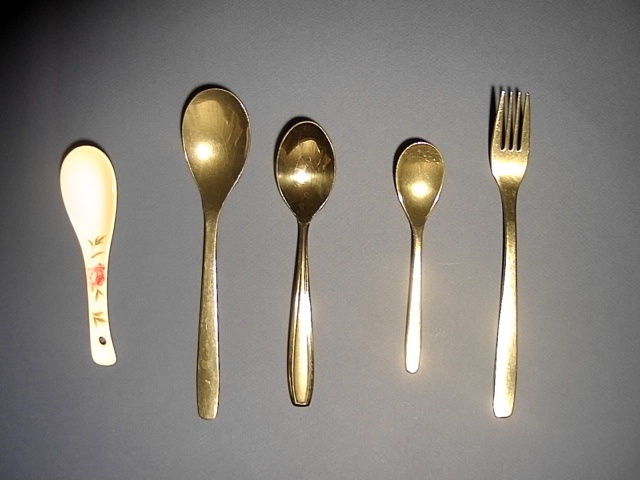
\includegraphics[width=\textwidth]{figures/separated_layout_example.jpg}
\caption{Separated layout (training condition)}
\label{fig:app-separated}
\end{subfigure}
\hfill
\begin{subfigure}{0.48\textwidth}
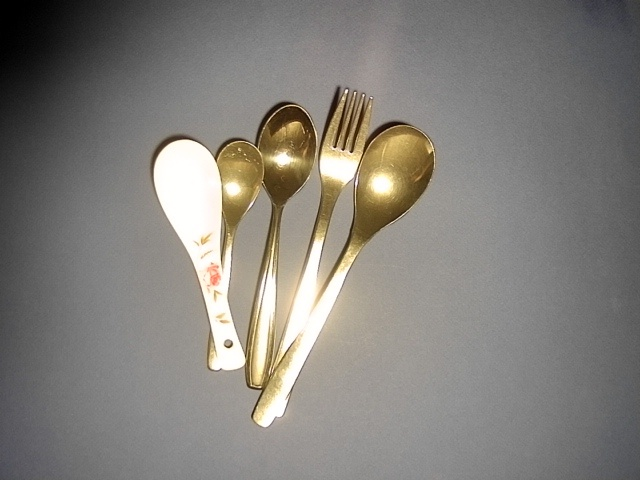
\includegraphics[width=\textwidth]{figures/overlay_layout_example.jpg}
\caption{Overlay layout (test condition)}
\label{fig:app-overlay}
\end{subfigure}
\caption{Example images from the separated-to-overlay experiment. The training set uses non-overlapping layouts; the test set uses overlapping layouts.}
\label{fig:app-separated-vs-overlay}
\end{figure}

\subsection{Real-Instrument Experiments}

The surgical kit proxy dataset contains six real instrument classes
(scissor1, scissor2, scissor3, scissor4, forcep, scalpel) photographed
on matte and reflective backgrounds across four sessions. Each image
contains exactly six instruments (one per class) in fixed positions per
session. Three staged experiments were trained with YOLO11s for
100~epochs.

Session-level splits were used for each experiment:
\texttt{matte\_train\_reflective\_test} trained on two matte-background
sessions and tested on two reflective-background sessions;
\texttt{reflective\_train\_matte\_test} reversed the backgrounds;
\texttt{shape\_similarity\_real\_proxy} trained on two sessions and
tested on a different held-out session. Training used the same
configuration as the brightness experiments (YOLO11s, 640$\times$640,
100~epochs, batch~16, deterministic seed~42, no augmentation).

Table~\ref{tab:app-surgical-kit-per-class} shows the per-class AP50
breakdown. The pattern is diagnostic of position-cue learning: classes
that achieve high AP in one split fall to zero in others, matching
session-specific instrument positions rather than visual features.

\begin{table}[H]
\centering
\caption{Per-class AP50 for the three real-instrument experiments}
\label{tab:app-surgical-kit-per-class}
\small\renewcommand{\arraystretch}{1.2}\setlength{\tabcolsep}{4pt}
\begin{tabularx}{\textwidth}{lrrr}
\hline
Class & matte$\rightarrow$reflective & reflective$\rightarrow$matte & shape\_similarity \\
\hline
scissor1 & 0.000 & 0.000 & \textbf{0.862} \\
scissor2 & 0.435 & 0.000 & 0.000 \\
scissor3 & 0.000 & 0.000 & 0.000 \\
scissor4 & 0.000 & 0.000 & 0.587 \\
forcep & 0.517 & 0.000 & 0.000 \\
scalpel & 0.446 & \textbf{0.717} & 0.069 \\
\hline
\end{tabularx}
\end{table}

Figure~\ref{fig:app-failure-mode} shows the most striking failure
mode: the \texttt{reflective\_train\_matte\_test} model detects only
the scalpel (the most visually distinct instrument) and misses all five
remaining classes. The confusion matrix for the
\texttt{shape\_similarity\_real\_proxy} experiment
(Figure~\ref{fig:app-confusion}) confirms that class associations are
split-specific rather than shape-driven.

\begin{figure}[H]
\centering
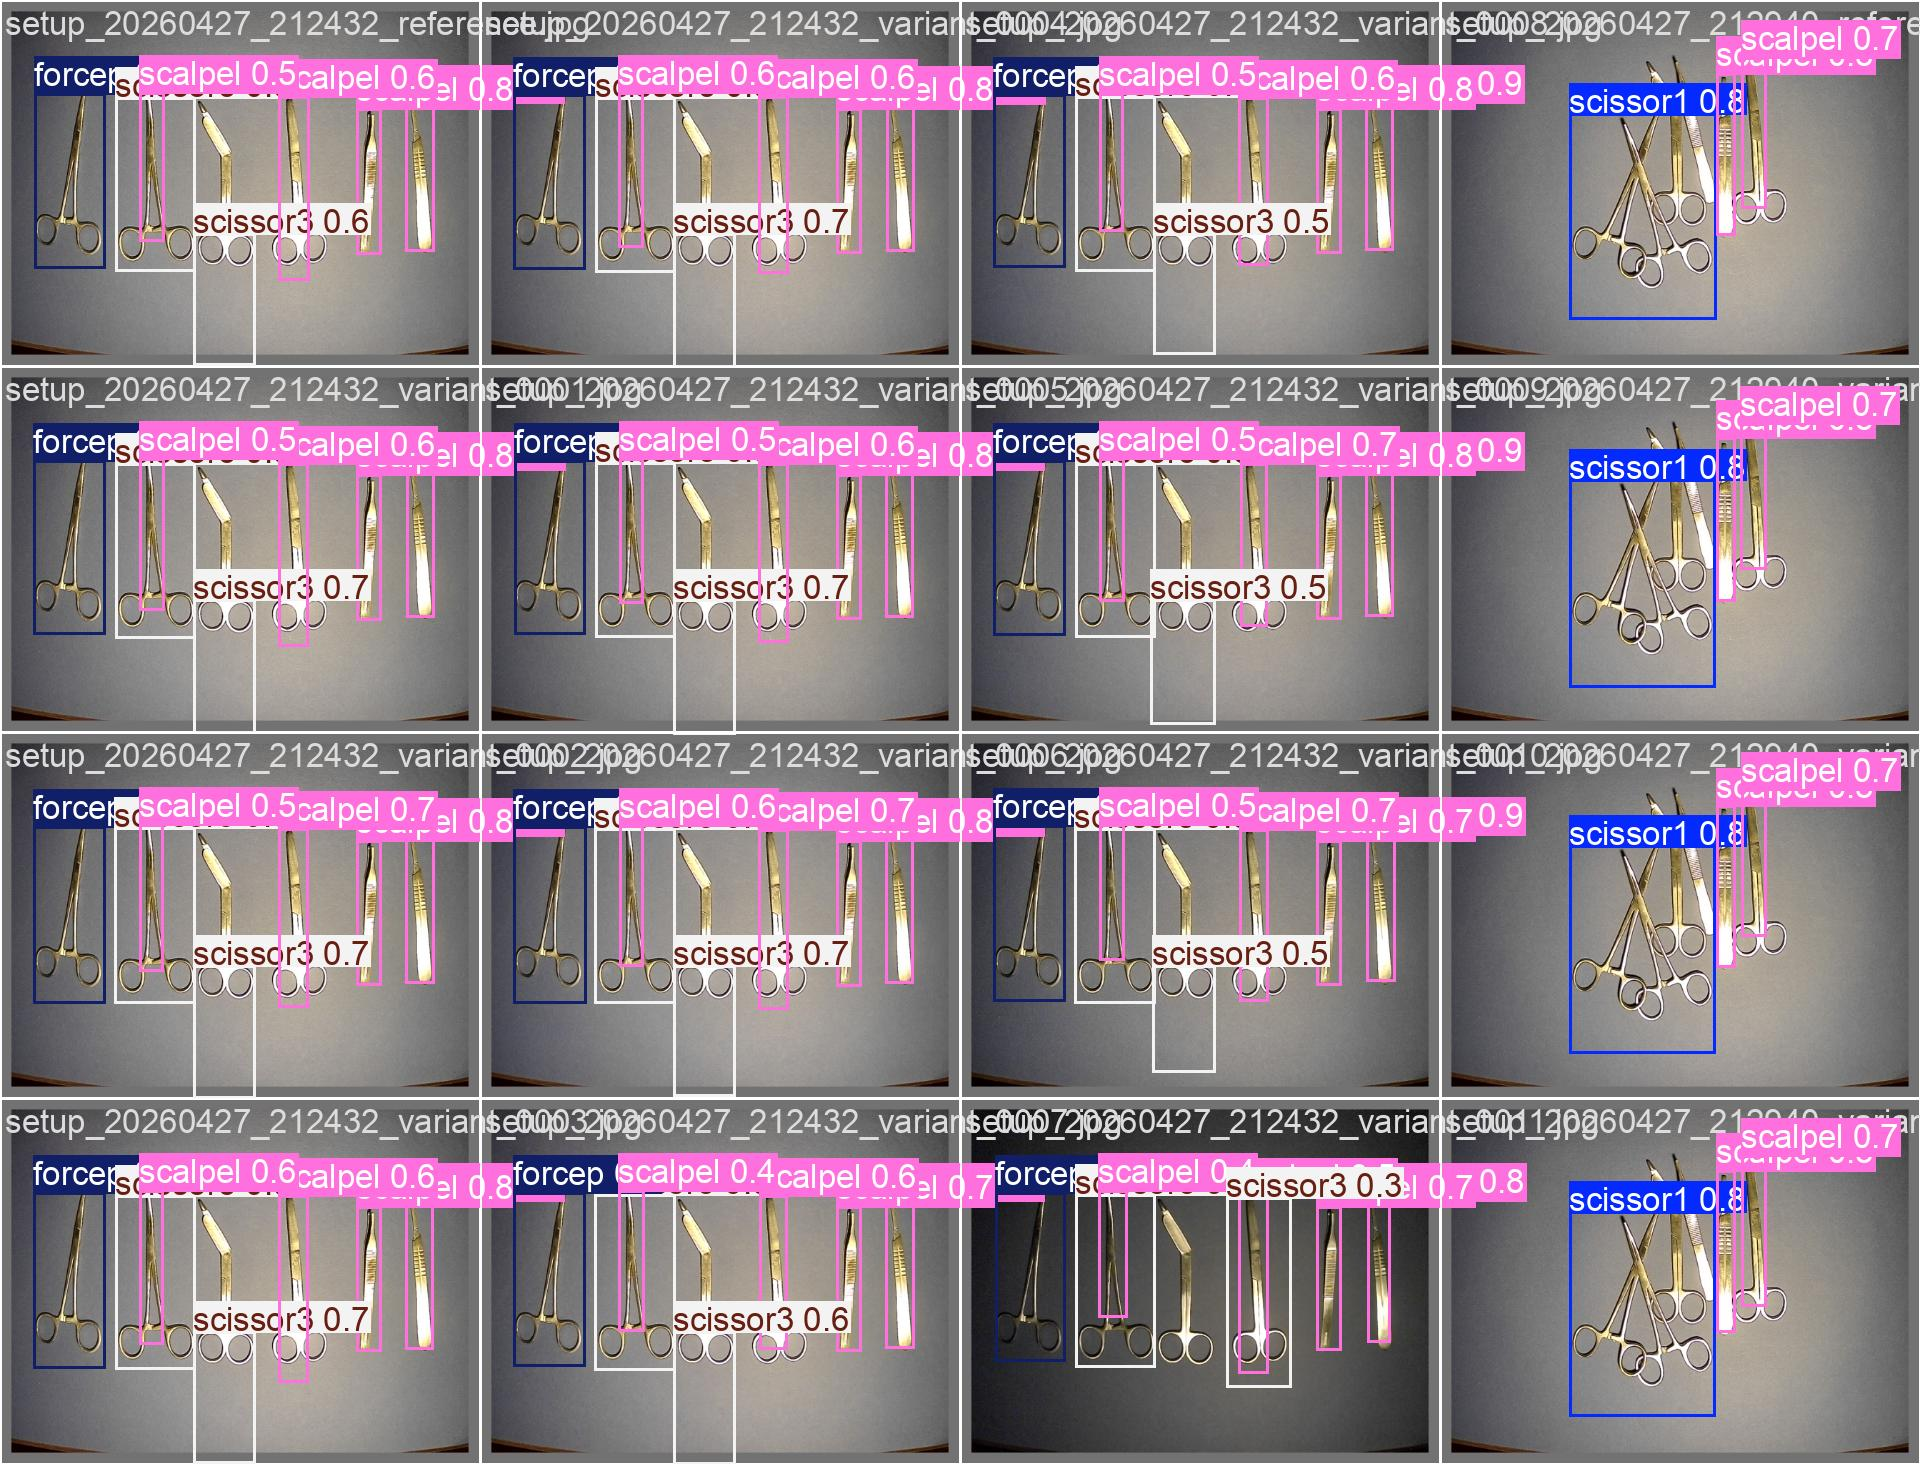
\includegraphics[width=\textwidth]{figures/val_batch0_pred.jpg}
\caption{Prediction example from \texttt{reflective\_train\_matte\_test}. Only the scalpel is detected (bounding box); the other five instruments (scissor1--4, forcep) are all missed.}
\label{fig:app-failure-mode}
\end{figure}

\begin{figure}[H]
\centering
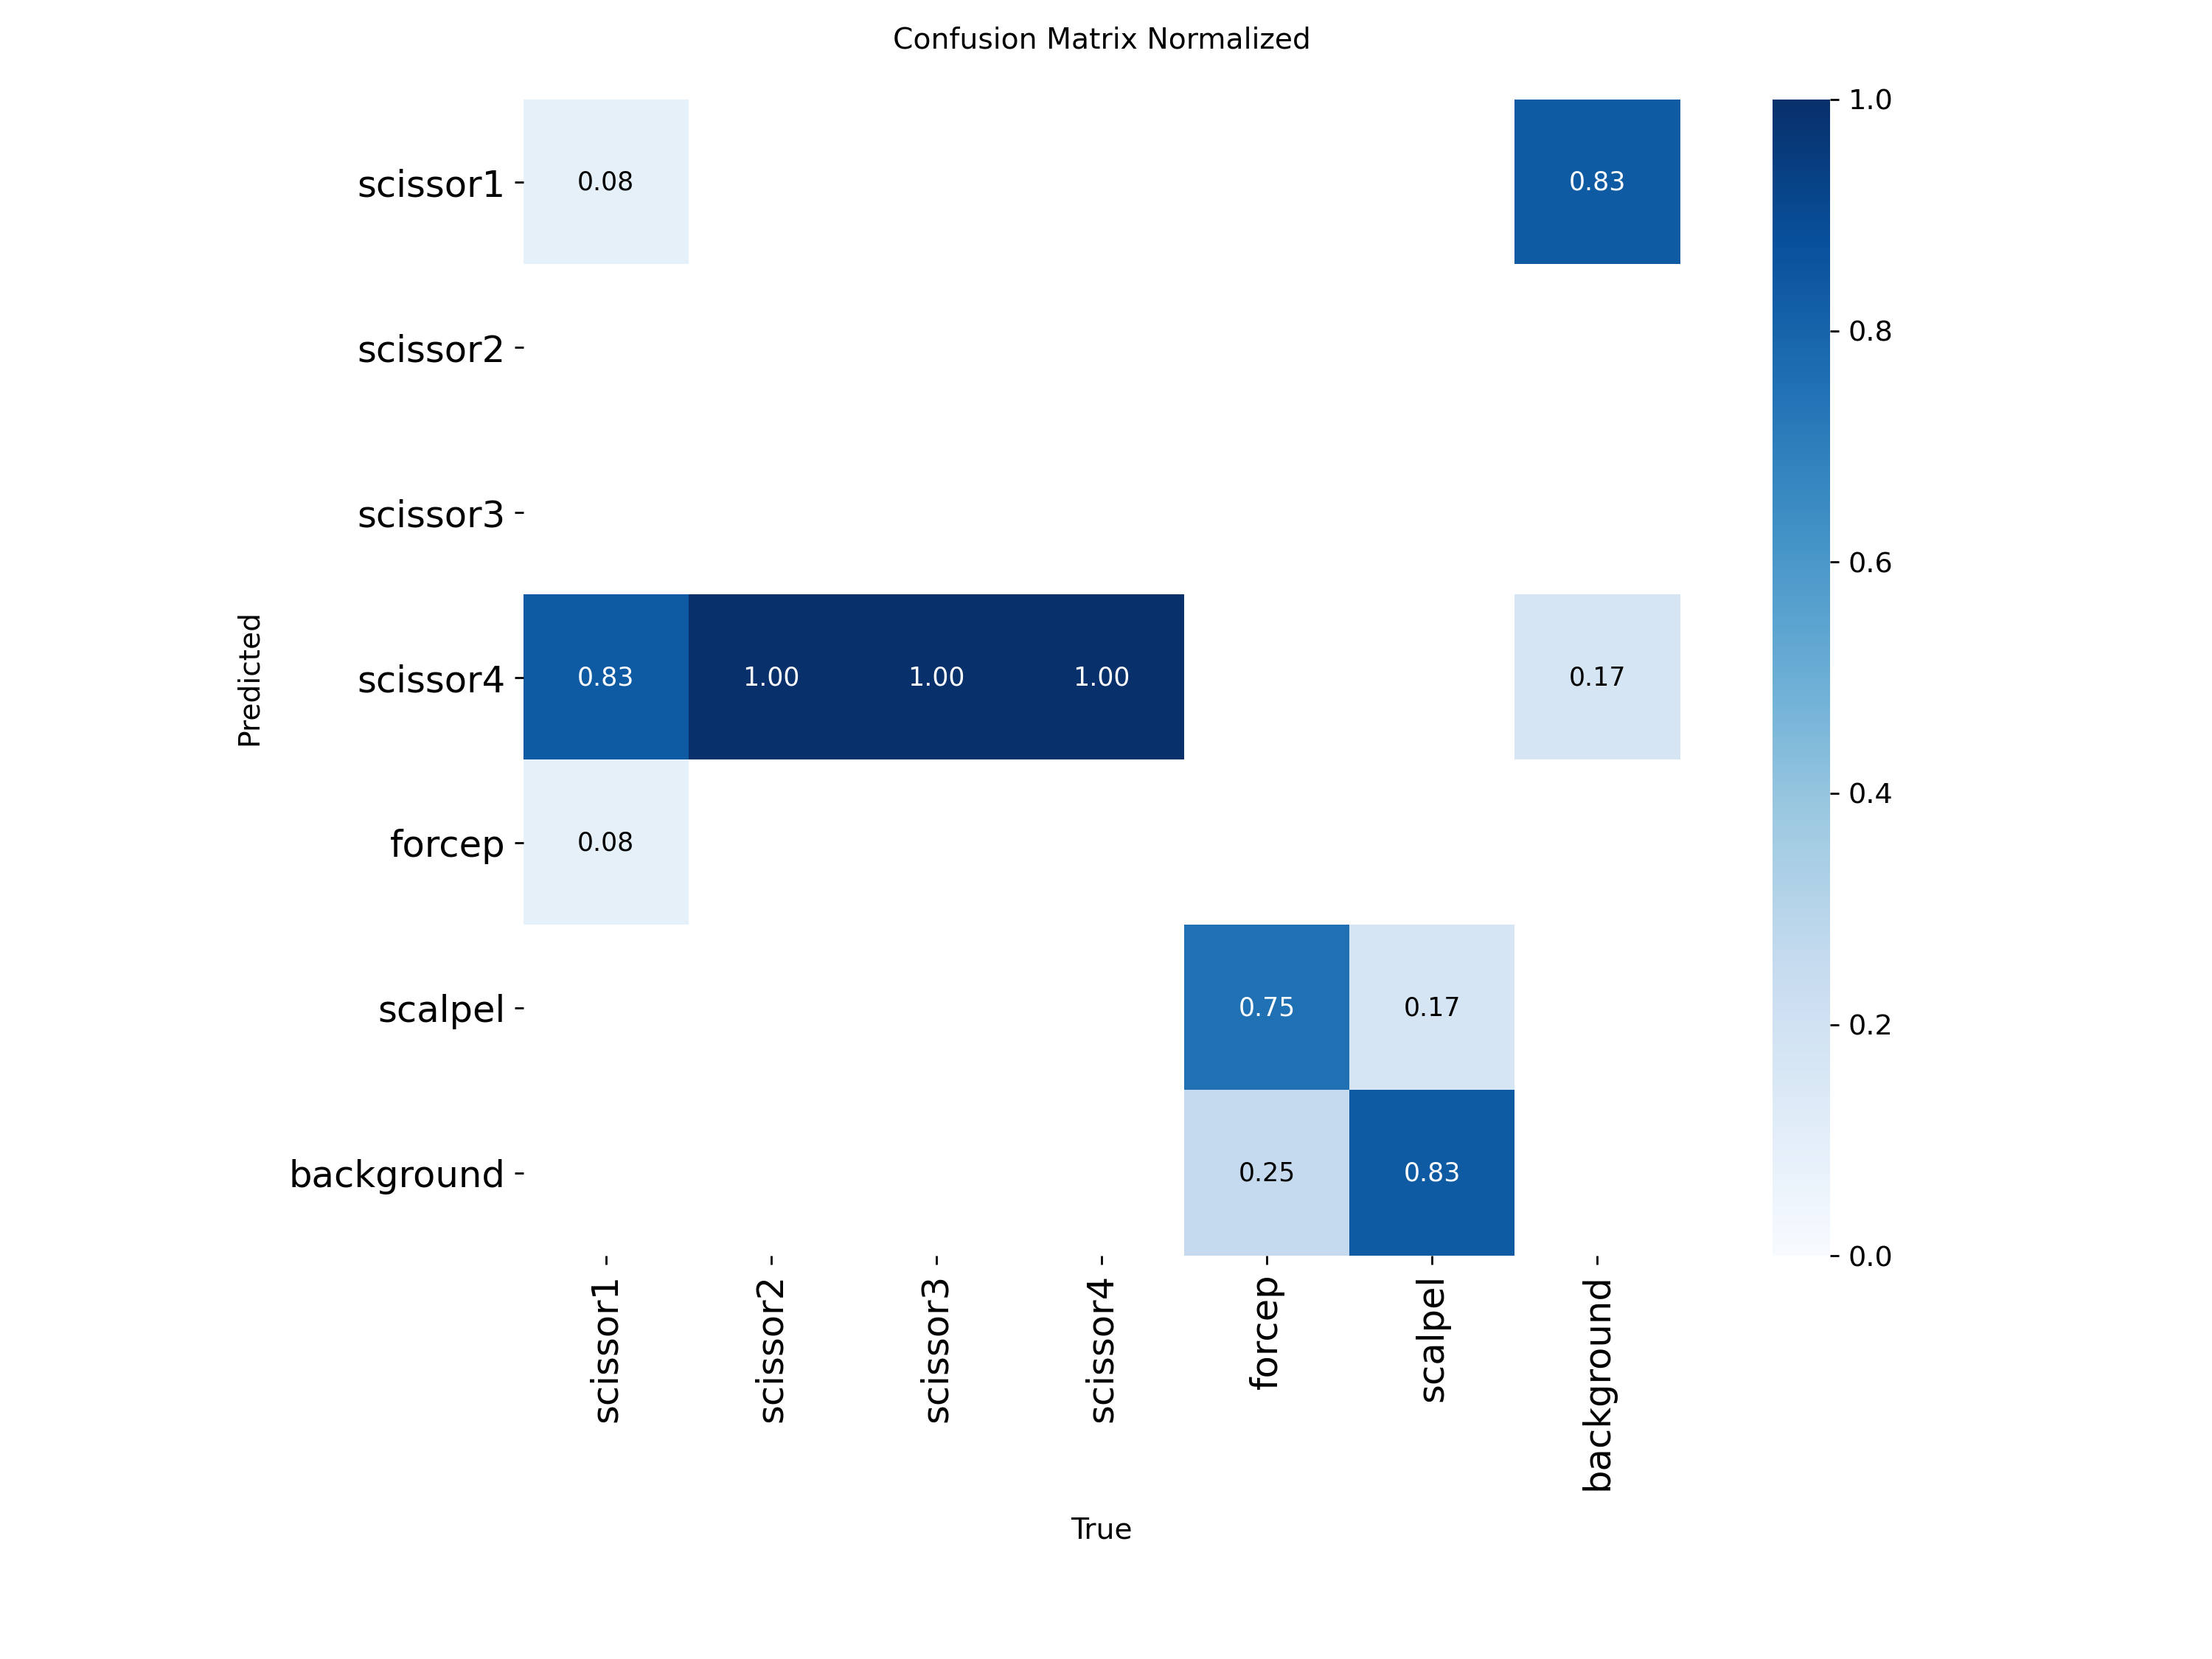
\includegraphics[width=0.75\textwidth]{figures/confusion_matrix_normalized.png}
\caption{Normalized confusion matrix for \texttt{shape\_similarity\_real\_proxy}. scissor1 and scissor4 are the only classes with nonzero true-positive rates; the remaining classes are uniformly missed.}
\label{fig:app-confusion}
\end{figure}

\begin{lstlisting}[caption={Train the three surgical kit stages},label=lst:train-surgical]
uv run bash scripts/train_surgical_kit.sh
\end{lstlisting}

\begin{lstlisting}[caption={Re-evaluate all surgical kit stages},label=lst:validate-surgical]
uv run python scripts/eval_surgical_kit.py
\end{lstlisting}

\subsection{Lighting Diversity Experiment}
\label{sec:appendix-c-lighting-diversity}

Three YOLO11s models were trained on a self-collected spoon dataset
(three classes: spoon1, spoon2, spoon3) with increasing lighting
diversity: reference desk lamp only, reference plus 45-degree handheld
flashlight, and reference plus both 45- and 90-degree flashlight.
Each model was trained for 100~epochs at 640$\times$640. Held-out test
images were captured under intermediate flashlight angles not seen in
any training set. Each additional lighting condition improved all
metrics (Table~\ref{tab:app-lighting-diversity}).

\begin{table}[H]
\centering
\caption{Lighting diversity experiment results}
\label{tab:app-lighting-diversity}
\small\renewcommand{\arraystretch}{1.2}\setlength{\tabcolsep}{4pt}
\begin{tabularx}{\textwidth}{lrrrr}
\hline
Training conditions & P & R & mAP50 & mAP50-95 \\
\hline
Reference only & 0.951 & 0.998 & 0.995 & 0.923 \\
Reference + 45$^\circ$ & 0.998 & 1.000 & 0.995 & 0.987 \\
Reference + 45$^\circ$ + 90$^\circ$ & 0.999 & 1.000 & 0.995 & 0.990 \\
\hline
\end{tabularx}
\end{table}

\begin{lstlisting}[caption={Train lighting diversity models},label=lst:train-lighting]
uv run bash scripts/train_lighting_diversity.sh
\end{lstlisting}

\begin{lstlisting}[caption={Re-evaluate lighting diversity models},label=lst:validate-lighting]
uv run python scripts/eval_lighting_diversity.py
\end{lstlisting}

% ── Appendix B: Bills of Materials ──

\section{Bills of Materials}

\begin{table}[H]
\centering
\caption{Bills of materials}
\label{tab:bills-of-materials}
\small\renewcommand{\arraystretch}{1.2}\setlength{\tabcolsep}{4pt}
\begin{tabularx}{\textwidth}{|>{\raggedright\arraybackslash}p{1cm}|>{\raggedright\arraybackslash}X|>{\raggedright\arraybackslash}p{1.2cm}|>{\raggedright\arraybackslash}p{1cm}|>{\raggedright\arraybackslash}X|>{\raggedright\arraybackslash}p{1.2cm}|>{\raggedright\arraybackslash}p{1.2cm}|}
\hline
Item & Description & Qty & Unit & Supplier & Unit Cost & Extended \\
\hline
1 & Cardstock paper (letter, 65 lb) & 1 & pack (50) & Office supply & \$8 & \$8 \\
2 & Clear adhesive sleeves & 1 & pack (100) & Office supply & \$10 & \$10 \\
3 & Foam backing board (20$\times$30 in) & 1 & sheet & Craft store & \$5 & \$5 \\
4 & AprilTag markers (printed on paper) & 30 & sheets & In-house & \$0 & \$0 \\
5 & Laptop or tablet for scanning & 1 & unit & Existing & \$0 & \$0 \\
6 & Camera stand (optional) & 1 & unit & Online & \$20 & \$20 \\
7 & Printed study flashcards & 30 & sheets & In-house & \$0 & \$0 \\
8 & Assorted office supplies (tape, scissors, binder clips) & 1 & set & Office supply & \$10 & \$10 \\
\hline
\multicolumn{6}{|p{0.8\textwidth}|}{\textbf{Total prototype material cost}} & \textbf{\$53} \\
\hline
\end{tabularx}
\end{table}

Alternative material options and their current market prices are documented as
cost-reference sources: stainless steel work tables~\cite{atosa-stainless-table-accessed-2026,
california-cooking-table-accessed-2026}, stainless steel sheet stock~\cite{best-metal-products-stainless-sheet-accessed-2026},
HDPE cutting board~\cite{us-plastic-hdpe-accessed-2026}, camera copy stands~\cite{cambo-accessed-2026,
meiji-techno-accessed-2026}, surface liners~\cite{contact-shelf-liner-accessed-2026,
contact-stainless-liner-accessed-2026}, board materials~\cite{home-depot-project-panels-accessed-2026,
office-depot-foam-board-accessed-2026, poster-board-walmart-accessed-2026}, and
CPI-adjusted cost references~\cite{bls-cpi-calculator-accessed-2026}.
These reflect upper-bound estimates; actual spending can be lower by reusing
existing equipment or substituting available materials.

The primary project cost is labor: module authoring, software implementation,
experimental data collection, study moderation, analysis, and report writing.
These are captured in the project plan's task assignments and are not itemized
as direct material purchases. The prototype is designed to work with materials
already available in a typical academic or office environment.



% ── Appendix C: Sample Instrument JSON ──

\section{Sample Instrument JSON}
\label{app:sample-instrument-json}

The instrument record below shows the data model fields for one
required tray item.

\begin{lstlisting}
{
  "id": "fgvc12_major_scissors_mayo_straight_7in",
  "display_name": "Scissors Mayo Straight 7\"",
  "family": "Cutting/dissecting",
  "aliases": [
    "SCISSORS MAYO STRAIGHT 7\"",
    "JARIT_101-220"
  ],
  "distinguishing_features": [
    "Heavy straight blades, semi-blunt tips",
    "Heavier, broader blade profile than Metzenbaum scissors",
    "Ring-handled cutting instrument"
  ],
  "common_confusions": [
    "fgvc12_major_scissors_mayo_curved_7in",
    "fgvc12_major_scissors_metz_curved_7in"
  ],
  "image_refs": [
    {
      "id": "view_a",
      "path": "data/instruments/fgvc12_major_tray_v1/fgvc12_major_scissors_mayo_straight_7in_view_a.jpg",
      "source": "fgvc12_google_drive_major_tray",
      "approved_for_study": true,
      "approved_for_assessment": false,
      "attribution": "FGVC12 shared Google Drive major tray image"
    }
  ],
  "apriltag_id": 0,
  "card_front_policy": "neutral_assessment_front",
  "notes": "FGVC12 major tray class JARIT_101-220. Expert review pending before assessment use.",
  "local_verification_status": "pending_review"
}
\end{lstlisting}

% ── Appendix D: FGVC12 Module Instrument Set ──

\section{FGVC12 Module Instrument Set}
\label{app:fgvc12-instrument-table}

\begin{table}[H]
\centering
\caption{FGVC12 module instrument set, by family, with distinguishing features and lookalike relationships}
\label{tab:fgvc12-module-instruments}
\small\renewcommand{\arraystretch}{1.2}\setlength{\tabcolsep}{3pt}
\begin{tabularx}{\textwidth}{|>{\raggedright\arraybackslash}X|>{\raggedright\arraybackslash}X|>{\raggedright\arraybackslash}X|}
\hline
Instrument & Distinguishing features & Lookalike(s) \\
\hline
\multicolumn{3}{|>{\centering\arraybackslash}X|}{\textbf{Cutting / dissecting}} \\
\hline
Mayo scissors straight 7'' & Heavy straight blades, semi-blunt tips & Mayo curved 7'' \\
Mayo scissors curved 7'' & Heavy curved blades, broader than Metzenbaum & Metzenbaum curved 7'' \\
Metzenbaum scissors curved 7'' & Slim lightweight blades for delicate tissue & Mayo curved 7'', Metz curved 10'' \\
Metzenbaum scissors curved 10'' (distractor) & Same slim design, longer shaft & Metzenbaum curved 7'' \\
Knife handle \#3 short & Short handle, accepts \#3 blade & --- \\
\hline
\multicolumn{3}{|>{\centering\arraybackslash}X|}{\textbf{Clamping / occluding}} \\
\hline
Kelly clamp 6'' & Serrations on distal half of jaw & Crile curved, Kelly 8'' \\
Crile clamp curved 5.5'' & Serrations run full jaw length & Kelly 6'' \\
Kocher clamp 6'' & Single tooth at tip, full serrations & --- \\
Allis clamp 6'' & Multiple interlocking teeth & Babcock 6'' \\
Babcock clamp 6'' & Smooth fenestrated jaws & Allis 6'' \\
Kelly clamp 8'' (distractor) & Distal-half serrations, longer overall & Kelly 6'' \\
Babcock clamp 9.5'' (distractor) & Larger smooth fenestrated jaws & --- \\
\hline
\multicolumn{3}{|>{\centering\arraybackslash}X|}{\textbf{Grasping / holding}} \\
\hline
Adson forceps w/ teeth & Short, 1$\times$2 teeth at tip & DeBakey 8'' \\
DeBakey forceps 8'' thoracic tip & Long, atraumatic longitudinal serrations & Adson w/ teeth \\
\hline
\multicolumn{3}{|>{\centering\arraybackslash}X|}{\textbf{Suturing}} \\
\hline
Mayo-Hegar needle holder 7'' & Short heavy jaws, cross-serration & Mayo-Hegar 8'' \\
Mayo-Hegar needle holder 8'' (distractor) & Same, longer shaft & Mayo-Hegar 7'' \\
\hline
\end{tabularx}
\end{table}

% ── Appendix E: System Design Reference Tables ──
\newpage
\section{System Design Reference Tables}
\label{app:system-design-reference-tables}

\begin{table}[H]
\centering
\caption{Data model objects and required fields}
\label{tab:app-data-model-objects}
\small\renewcommand{\arraystretch}{1.2}\setlength{\tabcolsep}{4pt}
\begin{tabularx}{\textwidth}{|>{\raggedright\arraybackslash}X|>{\raggedright\arraybackslash}X|>{\raggedright\arraybackslash}X|}
\hline
Object & Required Fields & Why It Matters \\
\hline
\texttt{Instrument} & \texttt{id}, \texttt{display\_name}, \texttt{family}, \texttt{aliases}, \texttt{distinguishing\_features}, \texttt{image\_refs}, \texttt{apriltag\_id}, \texttt{local\_verification\_status} & Supports retrieval cards, quiz prompts, card scanning, and local naming. \\
\hline
\texttt{TrayTemplate} & \texttt{id}, \texttt{name}, \texttt{version}, \texttt{procedure\_family}, \texttt{source\_note}, \texttt{required\_items}, \texttt{distractor\_items}, \texttt{lookalike\_pairs}, \texttt{assessment\_variants} & Stores the local count-sheet task and separates required instruments from distractors. \\
\hline
\texttt{TrayItemRequirement} & \texttt{instrument\_id}, \texttt{quantity}, \texttt{reference\_number}, \texttt{location\_or\_layer}, \texttt{acceptable\_substitutes}, \texttt{notes} & Mirrors real count-sheet fields and makes count/location errors measurable. \\
\hline
\texttt{AssessmentVariant} & \texttt{id}, \texttt{mode}, \texttt{random\_seed}, \texttt{required\_item\_ids}, \texttt{distractor\_item\_ids}, \texttt{card\_front\_policy}, \texttt{feedback\_enabled} & Keeps pre/post/delayed tasks comparable while preventing answer leakage. \\
\hline
\texttt{LearningRun} & \texttt{run\_id}, \texttt{learner\_id\_hash}, \texttt{participant\_group}, \texttt{tray\_template\_id}, \texttt{variant\_id}, \texttt{mode}, \texttt{started\_at}, \texttt{completed\_at} & Separates study, quiz, practice, pre-test, post-test, and delayed attempts. \\
\hline
\texttt{DetectedCard} & \texttt{run\_id}, \texttt{apriltag\_id}, \texttt{instrument\_id}, \texttt{timestamp}, \texttt{detection\_confidence}, \texttt{confirmed\_by\_user} & Lets marker failures be audited instead of silently counted as learner errors. \\
\hline
\texttt{AttemptResult} & \texttt{run\_id}, \texttt{selected\_items}, \texttt{duration\_seconds}, \texttt{accuracy\_score}, \texttt{required\_recall}, \texttt{errors}, \texttt{confidence\_summary} & Provides the main pre/post evidence. \\
\hline
\texttt{ItemResult} & \texttt{run\_id}, \texttt{instrument\_id}, \texttt{required\_qty}, \texttt{selected\_qty}, \texttt{error\_category}, \texttt{confidence}, \texttt{not\_sure} & Supports item-level feedback, weak-item review, high-confidence error reporting, and instructor review. \\
\hline
\end{tabularx}
\end{table}

\begin{table}[H]
\centering
\caption{Feature-to-evidence mapping for the learning loop}
\label{tab:app-feature-to-evidence}
\small\renewcommand{\arraystretch}{1.2}\setlength{\tabcolsep}{4pt}
\begin{tabularx}{\textwidth}{|>{\raggedright\arraybackslash}X|>{\raggedright\arraybackslash}X|>{\raggedright\arraybackslash}X|}
\hline
Feature & Evidence-based role & Engineering requirement \\
\hline
Retrieval-first study cards & Initial instruction that still asks the learner to answer before reveal & Store photos, names, aliases, functions, distinguishing features, and local notes; present prompts before explanations \\
\hline
Identification quiz & Central retrieval practice for instrument identity and features & Ask recall or recognition questions, randomize distractors, record correctness, confidence, and time \\
\hline
Simulated tray sorting & Safe applied retrieval in a realistic work task & Let learners assemble or check a tray against a count sheet in a low-risk training environment \\
\hline
Immediate error-specific feedback & Deliberate practice and error correction & Explain wrong answers and classify errors as missing, extra, wrong, misidentified, or wrong count \\
\hline
Confidence ratings & Metacognitive signal for learner and instructor & Capture confidence before or after tasks so low-confidence correct answers and high-confidence errors are visible \\
\hline
Separated pre/post tests & Evaluation not contaminated by coaching & Disable hints and feedback during tests; export comparable pre/post accuracy, time, error type, and confidence \\
\hline
\end{tabularx}
\end{table}

\begin{table}[H]
\centering
\caption{Real tray list examples and design implications}
\label{tab:app-real-tray-examples}
\small\renewcommand{\arraystretch}{1.2}\setlength{\tabcolsep}{4pt}
\begin{tabularx}{\textwidth}{|>{\raggedright\arraybackslash}X|>{\raggedright\arraybackslash}X|>{\raggedright\arraybackslash}X|}
\hline
Real Example & What It Shows & Design Implication \\
\hline
Stryker Gamma4 Indication Tray count sheet & A real vendor count sheet uses tray name, insert/base sections, reference numbers, descriptions, locations, quantities, check boxes, total instrument counts, additional items, and hospital signature \cite{stryker-gamma4-count-sheet-2023}. & TrayGuard should store \texttt{reference\_number}, \texttt{description/display\_name}, \texttt{location\_or\_layer}, \texttt{quantity}, and \texttt{additional\_items} fields even if the first module only uses names and quantities. \\
\hline
Stryker IMN Basic Instruments Tray count sheet & A second real count sheet uses the same pattern and splits the tray into insert/base groupings with total counts of 15 and 10 instruments \cite{stryker-imn-count-sheet-2023}. & The data model should support sections/layers and total-count validation, not just a flat list. \\
\hline
Multi-specialty tray rationalization project & Rubak et al. consolidated, separated, or restructured 1{,}340 different instrument trays across surgical specialties at one university hospital, finding that different specialties required different tray structures \cite{rubak-et-al-2024}. & Real tray lists scale to thousands of configurations in a single hospital. The data model must be open-ended beyond the first study's 8--12 required concepts. \\
\hline
Published major orthopedic tray study & Toor et al. observed an 88-instrument major orthopedic tray across 80 procedures and compared optimized tray configurations of 47, 67, and 51 instruments \cite{toor-et-al-2022}. & Real clinical trays can be far larger than the first module. The first study should use 8-12 required concepts for feasibility, while preserving fields that can scale to larger trays. \\
\hline
\end{tabularx}
\end{table}

% ── Appendix F: Collaboration Task Matrix ──

\section{Collaboration Task Matrix}

\begin{table}[H]
\centering
\caption{Collaboration task matrix}
\label{tab:collaboration-task-matrix}
\small\renewcommand{\arraystretch}{1.2}\setlength{\tabcolsep}{4pt}
\begin{tabularx}{\textwidth}{|>{\raggedright\arraybackslash}X|c|c|c|c|c|}
\hline
Section & Owen & Matthew & Andy & Jacob & Qiyu \\
\hline
§1. Executive Summary & & $\checkmark$ & & & \\
\hline
§2. Introduction And Project Overview & & $\checkmark$ & $\checkmark$ & $\checkmark$ & $\checkmark$ \\
\hline
§3. Problem Definition And Scope & & $\checkmark$ & $\checkmark$ & & $\checkmark$ \\
\hline
§4. First Attempt: A CV Tray Checker & ? & $\checkmark$ & $\checkmark$ & & \\
\hline
§5. Limitations of the CV Approach & & $\checkmark$ & $\checkmark$ & $\checkmark$ & $\checkmark$ \\
\hline
§6. Literature And Related Work & & $\checkmark$ & $\checkmark$ & $\checkmark$ & $\checkmark$ \\
\hline
§7. Requirements Definition & & $\checkmark$ & $\checkmark$ & $\checkmark$ & $\checkmark$ \\
\hline
§8. Final Product Concept And Design Rationale & & $\checkmark$ & $\checkmark$ & & $\checkmark$ \\
\hline
§9. System Design & & $\checkmark$ & & $\checkmark$ & \\
\hline
§10. Analysis & & $\checkmark$ & & & $\checkmark$ \\
\hline
§11. Evaluation And Validation Plan & & $\checkmark$ & & & \\
\hline
§12. Risk Assessment And Scope Boundaries & & $\checkmark$ & & & \\
\hline
§13. Broader Impacts And Ethics & & $\checkmark$ & & $\checkmark$ & $\checkmark$ \\
\hline
§14. Project Plan And Future Work & & $\checkmark$ & & & \\
\hline
§15. Discussion And Final Recommendations & & $\checkmark$ & & & \\
\hline
Appendices (A--G) & & $\checkmark$ & $\checkmark$ & $\checkmark$ & $\checkmark$ \\
\hline
\hline
\end{tabularx}
\end{table}

% ── Appendix G: Presentation Slides ──

\section{Presentation Slides}
\label{app:presentation-slides}

The comprehensive FDR presentation and the Elevator Pitch video are available
at the following links:

\begin{itemize}
    \item \textbf{Elevator Pitch (Video):}
          \url{https://youtu.be/30bxrNoa23U} \\
          (Google Drive: \url{https://drive.google.com/file/d/15l2KWpXAH9UFEOdb6wtsnnOunTfgylGf/view})
    \item \textbf{Comprehensive FDR Presentation:}
          \url{https://drive.google.com/file/d/1muxtr2ontcy-FiZCh2k6ihDTQCkmapwu/view}
\end{itemize}

\label{sec:references}
{\small
\raggedright
\bibliographystyle{IEEEtran}
\bibliography{trayguard_refs}}

\end{document}
